\documentclass[12pt]{report}

%\usepackage{fullpage}
\usepackage[margin=1.0in]{geometry}
\usepackage{graphicx} 
\usepackage{wrapfig}
\usepackage{color}
%\usepackage[usenames,dvipsnames,svgnames,table]{xcolor}
\usepackage{gensymb}
\usepackage[font={small}]{caption}
\usepackage[font=small]{subcaption}
% draft watermark
%\usepackage{draftwatermark}
%\SetWatermarkScale{5}
%\SetWatermarkLightness{0.9}
% bibliography things
\usepackage[numbers,sort&compress]{natbib} 
\usepackage[nottoc,numbib]{tocbibind}
\usepackage{notoccite}
% math things
\usepackage{amsmath} 

% special commands to be used in drafts for notes and annotations
%\newcommand{\fix}[1]{\textbf{\color{red}{#1}}}
%\newcommand{\rewrite}[1]{\textit{\color{blue}{#1}}}
%\newcommand{\note}[1]{\textit{\color{red}{#1}}}
%\newcommand{\del}[1]{\textit{\color{purple}{#1}}}
% $$$$$$$    custom commands for the document $$$$$$$$$
% prevent the following words from being hyphenated
\hyphenation{CURRENT}
% capitalize the following words in a special way
\providecommand\Matlab{\textsc{MATLAB}}

\begin{document}
\begin{titlepage}
\begin{center}
\vspace{6cm}
{\large \uppercase{Mechanism and Sensor Design for SUPERball, a Cable-Driven Tensegrity Robot} \\[1.0cm]}
{By \\[0.5cm] \large Andrew P. Sabelhaus \\[1.5cm]}
{A report submitted in partial satisfaction of the \\[0.4cm]
requirements for the degree of \\[0.4cm]
Masters of Science, Plan II \\[0.4cm]
in \\[0.4cm]
Mechanical Engineering \\[0.4cm]
at the \\[0.4cm]
University of California, Berkeley \\[1.5cm]}
{Committee in charge: \\[1.5cm]
\rule{10cm}{0.4pt} \\
Professor Alice M. Agogino, Chair \\[1.5cm]
\rule{10cm}{0.4pt}\\
Professor Dennis Lieu}
\vfill
{\large Fall Semester 2014}
\end{center}
\end{titlepage}
\begin{abstract}
\thispagestyle{plain}
\begin{center}
Mechanism and Sensor Design for SUPERball, a Cable-Driven Tensegrity Robot \\
by \\
Andrew P. Sabelhaus\\
Master of Science in Engineering -- Mechanical Engineering \\
University of California, Berkeley \\
Professor Alice M. Agogino, Chair
\end{center}

Mechanical design for cable-driven robots, especially those in tensegrity (tensile-integrity) tension networks, introduces a variety of challenges not found in other types of robotics; in particular, novel problems exist for cable routing, sensing, and actuation.
This work describes designs for SUPERball, the Spherical Underactuated Planetary Exploration Robot Ball, constructed at NASA Ames Research Center.
SUPERball is a proof-of-concept spherical tensegrity robot built to show dynamic rolling locomotion.
Engineering requirements for this robot are discussed, as are the evolution of those requirements into component specifications and then into detail designs.
Mechanism designs are presented for the unique modular rod-ends used in SUPERball, including the cable routing system and actuator.
Custom force gauges are developed, evaluated, and used to show proof-of-concept sensing on SUPERball.
Structural testing is performed to evaluate SUPERball's rod-end housing, and future improvements are discussed based on all these observations.
Finally, preliminary locomotion is shown, using the fully constructed SUPERball robot from these designs.

\pagenumbering{arabic}
\end{abstract}
\pagenumbering{roman}

% ACKNOWLEDGEMENTS 
\begin{center}
\begin{minipage}{0.75\linewidth}
\vspace{4cm}
{\centering \textbf{Acknowledgements} \\[2cm] \par}
Many, many thanks to Alice Agogino for her support, guidance, advice, and feedback on this report and all papers we have published together.
Also, thanks to the entire team at NASA Ames Research Center and the Intelligent Robotics Group, in particular, Vytas SunSpiral and Adrian Agogino for their project vision and financial support.
Thanks to Jonathan Bruce and Ken Caluwaerts, my partners in this project, without whom this mechanical design and manufacturing would not be possible.\\

Thanks to the many Master of Engineering students, undergraduate researchers, and collaborators at NASA and UC Berkeley who have contributed significantly to aspects of this work, especially Sarah Dobi, Roya Firoozi, Yangxin Chen, Dizhou Lu, Margaret (Yuejia) Liu, Brian Tietz Mirletz, In Won Park, Stephen Goodwin, Kyle Morse, Jeffrey Friesen, and Kyunam Kim. \\

Drew was supported by a National Science Foundation Graduate Research Fellowship, No. DGE1106400. Funding for the robot constructed in this report was provided by a NASA Innovative Advanced Concepts (NIAC) grant through NASA Prime Contract number NAS2-03144.
Thanks to the opportunities provided by the Fung Institute for Engineering Leadership at UC Berkeley, the Qualcomm Undergraduate Experience in Science and Technology, the NASA Space Technology Reserch Fellowship, the Idaho Space Grant, and the ReCare foundation for providing me with the opportunity to work with fabulous masters' students and undergraduate researchers.
\end{minipage}
\end{center}
\clearpage

\tableofcontents
\listoffigures
\listoftables
\clearpage

%%%%%%%%%%%%%%%%%%%%%%%%%%%%%%%%%%%%%%%%%%%%%%%%%%
% Actual document begins
%%%%%%%%%%%%%%%%%%%%%%%%%%%%%%%%%%%%%%%%%%%%%%%%%%

\pagenumbering{arabic}
%\linespread{1.5}
%\doublespacing

%\part{Background}

%%%%%%%%%%%%%%%%%%%%%%%%%%%%%%%%%%%%%%%%%%%%%%%%%
% Introduction: overview of concept, organization of report
%%%%%%%%%%%%%%%%%%%%%%%%%%%%%%%%%%%%%%%%%%%%%%%%

\chapter{Introduction}

The Spherical Underactuated Planetary Exploration Robot Ball (SUPERball) project out of NASA Ames Research Center has sought to develop basic engineering understandings of tensegrity systems for certain space exploration mission concepts.
SUPERball and its simulation models are 6-strut tensegrity icosahedra, with adjustable-length cables for the tension network.
Adjusting the lengths of these cables allows the structure to change shape; quick shape changes can build momentum to develop dynamic rolling locomotion~\cite{Iscen2013,iscen2014flop}.
Figure \ref{fig:overview} shows the final, fully-assembled prototype of SUPERball for which this report discussess the mechanical design.
The following section describes the system motivation, goals, and context of this hardware project.

\begin{wrapfigure}{R}{0.55\columnwidth}
  \begin{center}
  \vspace{-0.5cm}
    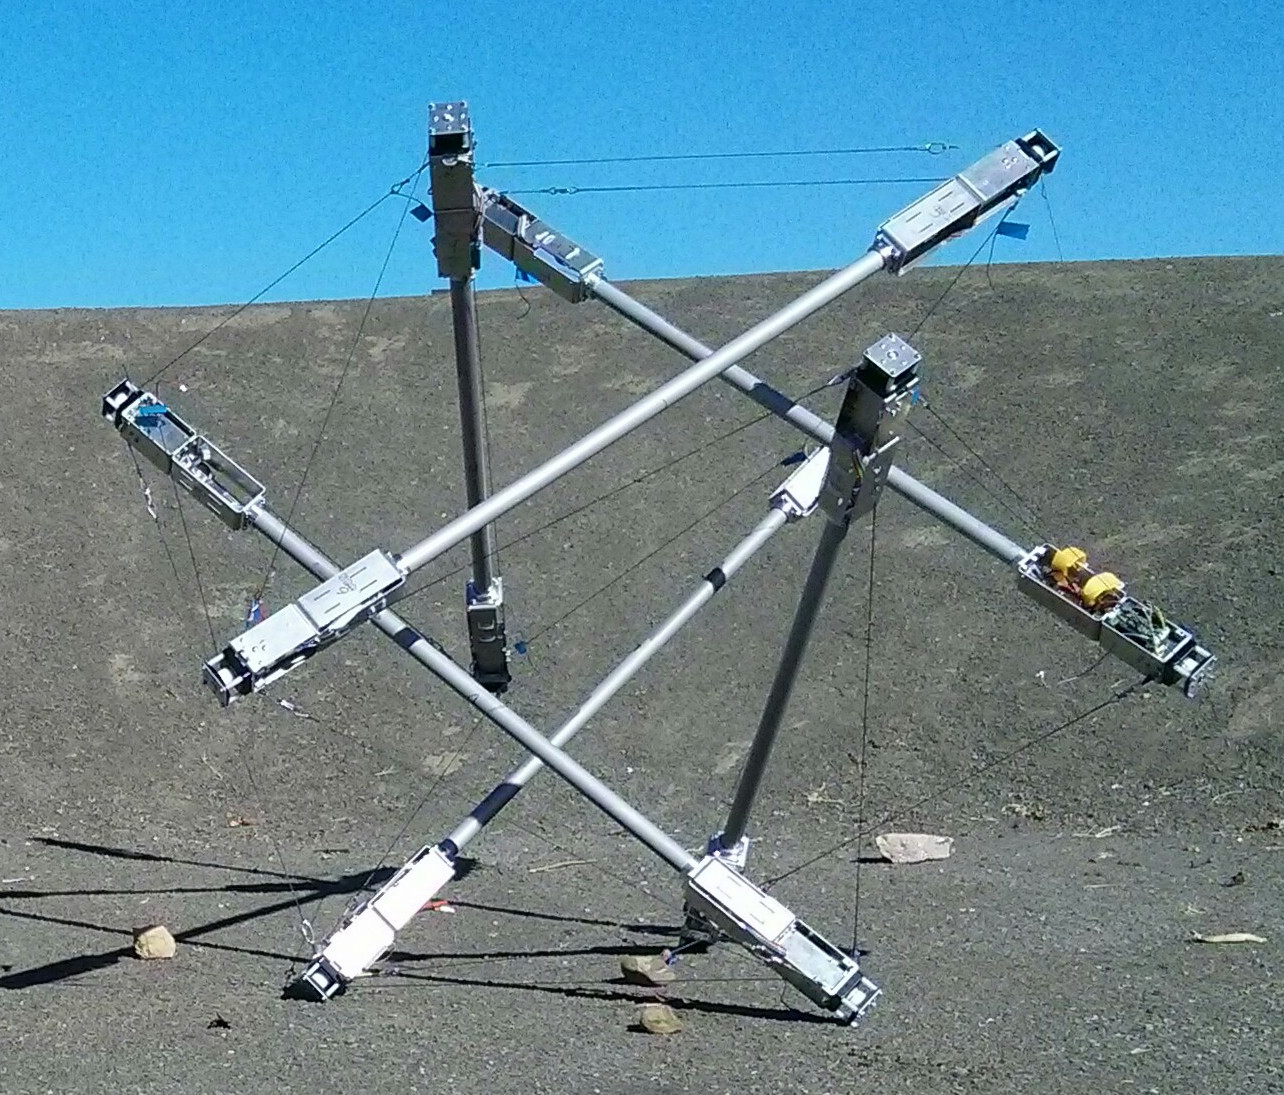
\includegraphics[width=0.53\textwidth]{img/superball_roverscape2_cropped.jpg}
    \caption{SUPERball, fully assembled, in the NASA Ames Research Center Roverscape.}
    \label{fig:overview}
  \end{center}
  \vspace{-0.7cm}
\end{wrapfigure}

This report is structured so as to emphasize the work that I completed as part of this master's degree.
However, as described in later chapters, multiple significant aspects of this robot's creation required work from many collaborators.
Consequently, the pronoun ``I'' is used to describe work which was primarily undertaken by myself for this degree, while ``We'' is used to describe collaborative work wherein I contributed less than approximately 80\% of the work.
Sections of this report which describe work that was collaborative are labelled explicitly.
However, for thoroughness' sake, these collaborative work areas are listed here.
The other authors, designers, and contributors are listed below according to their initials.
These fantastic folks are Jonathan Bruce (JB), Ken Caluwaerts (KC), Atil Iscen (AI), Sarah Dobi (SD), Roya Firoozi (RF), Yangxin Chen (YC), Yuejia/Margaret Liu (YL), and Dizhou Lu (DL).

\begin{itemize}
  \setlength{\itemsep}{0cm}%
  \setlength{\parskip}{0cm}%
  \item High-level hardware design: fully collaborative (JB, KC, and myself)
  \item Spring-Cable Mechanism initial high-level design (JB, KC)
  \item Actuator Housing initial high-level design (JB, KC)
  \item All simulation work and rolling locomotion trajectories (AI)
  \item Electronics, circuits, PCBs, and most embedded software (JB, KC)
  \item Experimental testing of SUPERball v1.5 prototype (YC, YL, DL)
  \item Torsional sensor test setup (SD, RF)
  \item Torsional sensor curve fitting and data analysis (JB)
\end{itemize}
 
The next section describes the motivation, background, context, and prior work for this project, including efforts before I joined.
Next, the engineering design process is discussed in the context of this odd, complicated system, and prototying approximations are specified.
The primary contributions of this work are then specified, in terms of mechanical designs, sensor designs, and testing procedures.
Finally, recent results are shown wherein SUPERball performs simple one-step locomotion.


%%%%%%%%%%%%%%%%%%%%%%%%%%%%%%%%%%%%%%%%%%%%%%%%%
% Second Chapter: Motivation, Background, Prior Work, Research Goals
%%%%%%%%%%%%%%%%%%%%%%%%%%%%%%%%%%%%%%%%%%%%%%%%

\chapter{Tensegrity Systems as Cable-Driven Robots}

\section{Background}

Though the field of mobile robotics continues to evolve at a rapid pace and new innvative robots are developed, certain challenges persist.
Out of these many challenges, two significant areas of interest are robot interaction with unknown environments/objects, and weight/volume/mass limitations of current robot design paradigms.
Traditional robot designs rely on moving joints (for manipulators), hard materials (metals, heavy plastics), and often, large boxy cages for centralized components.
Though high-performance robots such as Boston Dynamics' BigDog \cite{raibert2008bigdog} are constructed in this way, such design techniques regularly lead to heavy and bulky systems.
Additionally, such designs can be quite dangerous around sensitive objects such as humans, and either active compliance or other safety schemes are needed~\cite{garcia2007evolution,lefebvre2005active}.

Recent grants by funding agencies reflect this focus on new design paradigms, with an emphasis on unknown interactions and weight-reducing schemes.
The National Science Foundation begun offering the National Robotics Initiative grant in the 2011-2012 fiscal year, which focuses on co-robot technology for interactions between robots and delicate human actors~\cite{nsf2014national}.
Additionally, NASA has recently funded numerous research projects to make autonomous robots for space that are lighter (and thus cheaper) than current systems, including the CubeSats program~\cite{chin2008standardization,selva2012survey} and recent work at Stanford university for novel flywheel asteroid rovers~\cite{allen2013internally}.


\section{Motivation}
This work seeks to address these challenges by using new paradigms for structural and mechanical design.
As opposed to prior research into optimizing traditional designs for safety and weight, the new design paradigm of tensegrity structures can allow for novel solutions to safety and mass.
This research seeks to apply traditional engineering materials and manufacturing processes to break free from the bonds of moment arm transfer (e.g. through the joints of a manipulator) and dangerous interactions with unknown objects.

\section{Prior Work}

\subsection{Space Robotics and Planetary Landers}

Autonomous space exploration involves a variety of types of missions.
Beginning with static (non-mobile) landers such as Cassini and Huygens~\cite{matson2003cassini} and evolving into mobile wheeled robots such as Mars Curiosity~\cite{grotzinger2012mars}, the field has shifted towards autonomy and flexibility in lander design in order to get more science per mission.

However, even the most modern landers are still plagued with issues.
For example, one can identify three shortcomings of Mars Curiosity:

\begin{itemize}
  \setlength{\itemsep}{0cm}%
  \setlength{\parskip}{0cm}%
  \item Entry, Descent, and Landing systems. Wheeled rovers such as Mars Curiosity often require very delicate placement on a planet surface. Such systems may involve parachutes, retro-rockets, and/or airbag balloons. All of these require significant mass and engineering effort, raising the cost of missions, and reducing the amount of science per dollar.~\cite{Vytas_IPPW_2013,NIACfinalreport}
  \item High mass, low mass fraction. All landers are necessarily designed to produce science, and thus the ``mass fraction'' - or, the amount of mass used for science instruments versus the total system mass - is crucial. However, systems like Mars Curiosity have unfavorable mass fractions, due to a combination of factors.~\cite{Vytas_IPPW_2013,NIACfinalreport}
  \item Delicate systems that are prone to failure. Mobile wheeled robots such as Curiosity occassionally encounter unknown terrain, and if systems are not designed for such environments, they may fail. Of particular note are the punctures in Curiosity's wheels, which although do not disable the robot, are cause for concern.~\cite{Vytas_IPPW_2013,NIACfinalreport}
\end{itemize}

As mentioned before, recent funding for work to alleviate these issues implies a strong need for better solutions than wheeled robots.

\subsection{Tensegrity Structures}

Tensegrity (``tensile-integrity'') systems are colloquially defined as ``discontinuous compressive elements in a sea of tension''~\cite{fuller1962tensile}.
Tensegrity structures are entirely composed of pure tension and compression elements.
The subset of tensegrity systems discussed in this work are those which consist of only solid, axial rods (struts, in compression) held together without touching each other by a series of cables (in tension).
These are called class 1 tensegrity systems; this and other types are heavily explored in other work~\cite{C.R.1978,Skelton2009,sultan2002,Motro2003,Zhang2006a,BelHadjAli2010a}.
It can be shown mathematically that for an idealized class 1 tensegrity, no elements experience bending moments~\cite{skelton2001introduction}.
As a result, individual elements can be extremely lightweight: the only failure modes for these struts are simple axial compressive failure and failure from buckling.

A unique property of tensegrity structures is how they can internally distribute forces.  
As there are no lever arms, forces do not magnify into joints or other common points of failure.  
Rather, externally applied forces distribute through the structure via multiple load paths, creating a system level robustness and tolerance to forces applied from any direction.  
Thus tensegrity structures can be easily reoriented and are ideally suited for operation in dynamic environments where contact forces cannot always be predicted.

The SUPERball project does not seek to develop mathematical underpinnings of our system's dynamics, kinematics, or other mechanics.
These phenomena are well studied by the above texts.

\subsection{Tensegrity Robotics}

However, using tensegrity systems in robotics contexts is somewhat of a new concept, with authors in the field point to work by Paul and Lipson as the beginning of research into dynamically locomoting tensegrity systems in 2005 and 2006~\cite{Paul2005,Paul2006a}.
That work and others~\cite{miratstur2011athree-dof} focus more on dynamics and control than mechatronic design.

Mechanical design of tensegrity robots has only been explored in disparate contexts, with little formal methodology applied to prototyping and design, particularly for spherical robots like SUPERball.
To date, the majority of constructed tensegrity robots have been designed for open loop control, utilizing servo motors and limited sensing, and are often tethered for power and control~\cite{Koizumi2012b}, or have been secured to the ground~\cite{MiratsTur2010}.
Some related approaches utilize tensegrities as part of a larger, more complicated system, but not as the primary locomotion method~\cite{webster2013segmental}.
Others have created designs that do not use direct cable actuation, but instead produce forms of locomotion through structural vibration~\cite{khazanov2013exploiting}~\cite{bohm2013vibration}.
Finally, those that have demonstrated locomotion of icosahedral 6-strut tensegrity robots (such as SUPERball) have emphasized quasi-static movement over dynamic rolling~\cite{Shibata2009,Shibata2009a,Shibata2010}.

Other prior work from our team at NASA Ames Reseach Center has produced multiple robots which also develop novel movement, but again which were not designed using formal engineering practices but instead were simple prototypes.
The ReCTeR robot~\cite{Caluwaerts2013rsif,bruce2014design} is also a 6-strut icosahedral tensegrity, but it does not have the same actuation capabilities as SUPERball and is not designed to demonstrate dynamic rolling.
Other robots from NASA Ames that are not spherical include the TetraSpine and its revisions~\cite{Tietz2013,mirletz2014design}, the hardware of which shows limited undulatory snake-like motion.

Arguably, this work and the associated publications are the first to take a systematic, design-theoretic approach to developing prototype tensegrity hardware, especially that which is autonomous and designed for dynamic rolling locomotion~\cite{Caluwaerts2013rsif,sabelhaus2014hardware,bruce2014design,sabelhaus2015system}.

NASA had been interested in tensegrity robotics to attempt to overcome the challenges describe above for current planetary landers.
In particular, prior work from our group has shown the potential for a SUPERball-like system to land on Saturn's moon Titan without any outside EDL equipment - thus saving a significant amount of mass~\cite{Vytas_IPPW_2013,NIACfinalreport}.
A tensegrity robot can also address the other issues with wheeled Curiosity-like systems: a tensegrity robot will be lower mass (due to the lack of bending moment forces with respect to mechanical design), and is necessarily more resistant to unknown environments by design.
The research described in this report (system design for locomotion) is the other aspect to this landing work: it is desired to show that a SUPERball-like robot can both land and move on a planet or moon.


%\subsection{Cable-Driven Mechatronic Systems}
%This section hammers home the message of this report: I wanted to build a tensegrity system because it seemed like a novel methodology to address the motivation.
%However, in order to do this, I had to build a cable-driven system.
%Prior work was insufficient in some areas for our purposes: describe the prior things that people did for cable-driven robots.
%Address autonomy (others might not have to house their motors on the actual system).

\section{Research Goals}

As stated before, the singular purpose of this research is to show proof-of-concept dynamic rolling locomotion through cable tension/length change for 6-strut tensegrity robots.
SUPERball is this prototype.
Though there is only a single high-level goal, multiple other sub-goals exist.
Specifically, the following sub-goals were identified as milestones toward this larger vision:

\begin{itemize}
  \setlength{\itemsep}{0cm}%
  \setlength{\parskip}{0cm}%
  \item Specification of a reasonable design process for this robot that would transform high-level goals into engineering requirements
  \item Development of engineering designs that satisfied such requirements, particularly in the context of cable-driving mechanisms and sensors
  \item Development of sensors that would allow for full state estimation of the robot (with an eye toward future implementation of trajectory-tracking controllers)
  \item Testing of mechanisms and sensors to show reasonable prototype performance
\end{itemize}

These research goals are all address in the following sections, and although more work is to be done before dynamic rolling locomotion can occur, I and the other developers of SUPERball are optimistic about the design work that has occurred to date.

%%%%%%%%%%%%%%%%%%%%%%%%%%%%%%%%%%%%%%%%%%%%%%%%%%%%%%%%%%%%
% Third Chapter: Engineering Requirements and starting up things for SUPERball
%%%%%%%%%%%%%%%%%%%%%%%%%%%%%%%%%%%%%%%%%%%%%%%%%%%%%%%%%%%

\chapter{Engineering Requirements and Component Specifications for SUPERball}

At the time of this work, the task of developing sound design requirements for a full tensegrity robotic system which can achieve dynamic locomotion does not have a generally-accepted solution within the engineering community.
Most common design practices rely on models to transform engineering requirements into engineering specifications and specific component parameters \textcolor{blue}{CITE}; however, tensegrity robots such as SUPERball have relied on non-model-based machine learning methods for generating trajectories.
Since the primary goal of SUPERball was to show proof-of-concept that dynamic rolling locomotion is possible for this type of robot, the space of possible engineering requirements was vast: it is very possible for a variety of system configurations to be controlled to roll.
Thus, SUPERball is in a sense a controls-defined mechanical system: our engineering characteristics come from an iterative process of machine learning simulations paired with choices of discrete engineering components.
With the assistance of NASA's machine learning experts, this process was iterated over until a solution was found where the capabilities of engineering components matched the robot's simulated parameters.
Figure \ref{fig:design_process} and later sections explore this process of requirements generation.

\begin{figure}[thpb]
      \centering
      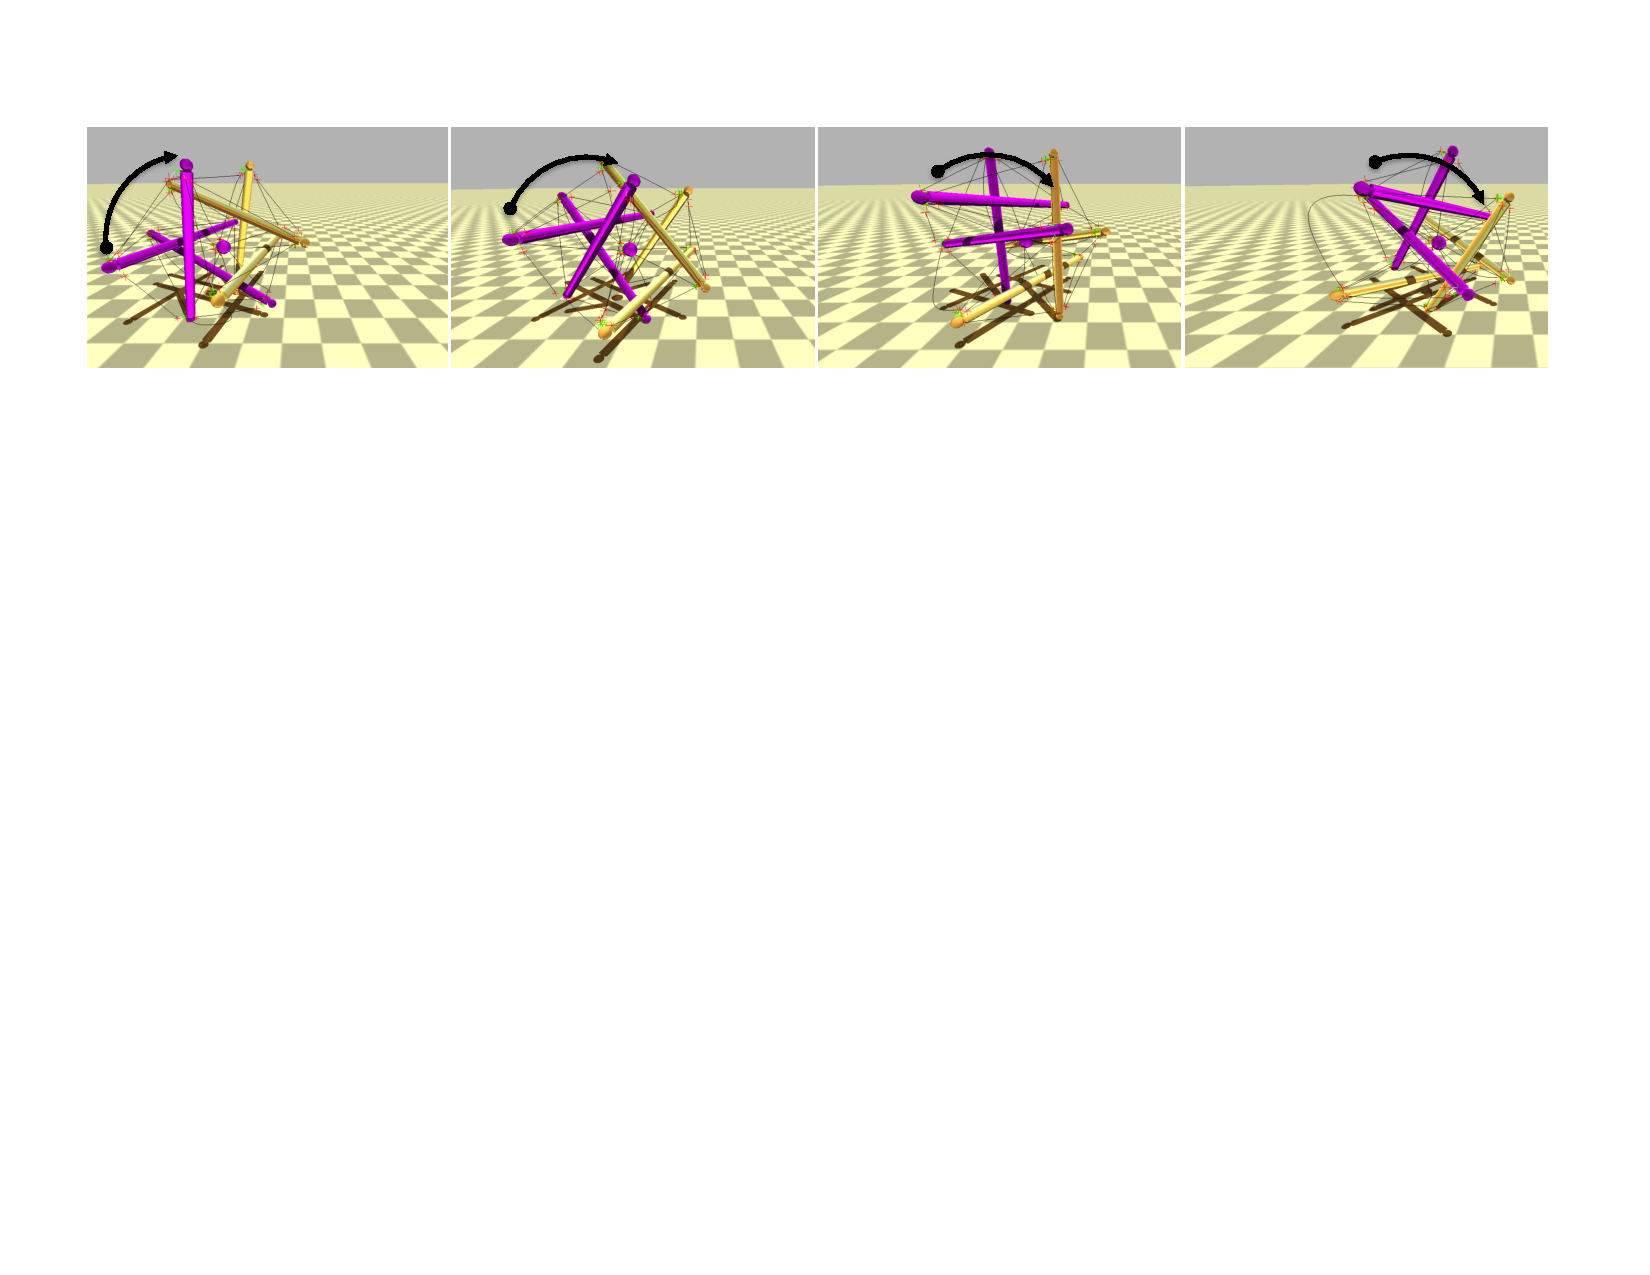
\includegraphics[width=0.9\columnwidth]{img/fig_rolling.pdf}
      \caption{A simulation of SUPERball in the NASA Tensegrity Robotics Toolkit, showing a machine-learned trajectory with fast dynamic rolling motion.}
      \label{fig:superball_rolling_ntrt}
      \vspace{-0.2cm}
\end{figure}

Of note is the use of the NASA Tensegrity Robotics Toolkit (NTRT) simulator for this machine learning. 
NTRT was developed for this use of simulating a tensegrity system's movement under changing input trajectories and patterns from reinforcement learning and evolutionary algorithms. \textcolor{blue}{CITE}.
Figure \ref{fig:superball_rolling_ntrt} shows such a machine-learned state trajectory replayed in NTRT.
The physical accuracy of NTRT and its underlying physics engine, Bullet Physics, were recently validated by our NASA team \textcolor{blue}{CITE}.

\section{Target Requirements for SUPERball Mechanisms}

Starting from the ill-defined goal of creating a structure that could produce rolling locomotion, a set of quantitative requirements was developed that can be related more directly to a given design specification.
At the time of generating these requirements, NTRT allowed for variations in the following parameters of a 6-strut spherical tensegrity model (like SUPERball):

\begin{wrapfigure}{R}{0.55\columnwidth}
  \begin{center}
  \vspace{-0.5cm}
    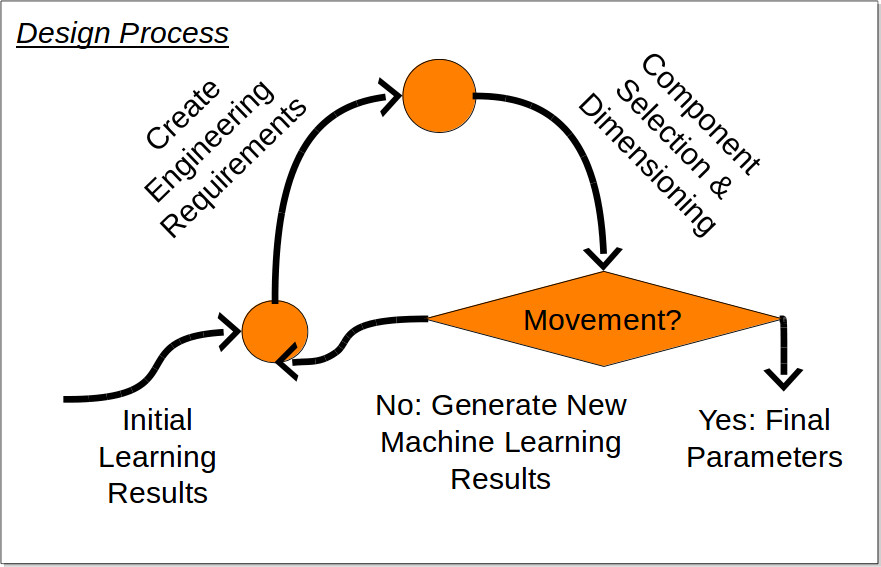
\includegraphics[width=0.53\textwidth]{img/design_process.jpg}
    \caption{Graphical representation of the informal design process used to generate requirements for SUPERball. This encapsulates the iteration over machine-learned trajectories paired with feasible realizations of robot hardware.}
    \label{fig:design_process}
  \end{center}
  \vspace{-0.7cm}
\end{wrapfigure}

\begin{itemize}
  \setlength{\itemsep}{0cm}%
  \setlength{\parskip}{0cm}%
  \item Actuator Maximum Torque (max $\tau$)
  \item Actuator Maximum Velocity (max $v$)
  \item Number of actuators ($n_{act}$)
  \item Strut Length ($l_{strut}$)
  \item Actuator Maximum Displacement (max $\Delta l$)
  \item Spring Constant of active and passive cables ($k_{active}, k_{passive}$)
  \item Strut Weight (Mass, $m$)
\end{itemize}

These parameters focus on the design of a single strut, though SUPERball consists of 6 identical rods and the negligably-lightweight cables which connect them.
This allowed iteration on a more limited subset of options which then automatically extrapolated into system-wide performance (as opposed to, for example, iterating over connectivity of the 6 struts, which would have introduced complex interactions between individual rod design and system-level configuration.)
Again, Figure \ref{fig:design_process} informally shows how our team performed this iteration.



Though this set of parameters (for each of which a requirement was generated) is relatively limited, it provided some greatly-needed grounding for the preliminary SUPERball design.
At the conclusion of iterating over these parameters, and comparing them to the possible choice of components for the robot, the quantitative requirements shown in Table \ref{tab:design_req} were created.
Again, these were iterated upon with other researchers until a reasonable level of convergence was acheived.
Note that some of these parameters in Table \ref{tab:design_req} exactly match the components listed later in Table \ref{tab:major_components}.
%Since these requirements were co-developed with the major engineering components of the robot, some requirements were post-specified after a solution was converged upon.
%The subset of strictly-defined a-priori parameters are highlighted in bold blue font in this table.

Additionally, certain relationships were established between parameters, allowing for more simplifying assumptions to be made.
For example, the actuator was assumed to be a spindle at the end of a motor that would draw in a flexible cable.
This allowed for the calculation of the maximum cable force from maximum motor torque.
Appendix \textcolor{blue}{BLAH} shows a spreadsheet of these calculations for reference.

\begin{table}[ht]
\caption{SUPERball preliminary design requirements, prior to v1.0 design.}%
\label{tab:design_req}%
\begin{center}%
%\resizebox{\columnwidth}{!}{%
\begin{tabular}{| c | c | c |}
\hline
Parameter & Specification & Units\\ \hline
Max $\tau$ & 3 & $Nm$ \\ \hline
Max v & 0.26 & $m/s$ \\ \hline
$n_{act}$ & 12 & actuators \\ \hline
$l_{strut}$ & 1.5 & $m$ \\ \hline
%Max $\Delta l$ &  & \\ \hline
%$k_{active}$ & & \\ \hline
%$k_{passive}$ & & \\ \hline
Strut Mass $m$ & 1.5 & kg \\ \hline
\end{tabular}%
%}
\end{center}
\end{table}

One particular parameter here deviates significantly from the intuitive expected result: only 12 of the possible 24 cables will have an actuator attached; the other 12 will be purely passive.
This is a design decision prompted singularly by mechanical design challenges of incorporating two actuation units per rod-end, and though it was justified using an NTRT simulation, still limits the functionality of SUPERball.

Finally, note that not all of the available parameters in NTRT were assigned an engineering requirement.
Some of these were deemed to be straightforward enough to incorporate during the detail design stage; for example, the maximum cable retraction length can be easily adjusted by changing the dimensions of the actuator housing and does not require a different COTS component.


%In Table \ref{tab:design_req}, $l_{strut}$ is the length of a strut, $\Delta l$ the rate of of length change (the change in rest length of the inline spring) of an actuated cable and $\max \tau$ the maximum spindle output torque.

\section{Preliminary Specification and Component Parameters}

Table \ref{tab:major_components} lists the major components of the robot that were selected to meet these requirements, as of the initial preliminary design.
These components were selected for focus during the preliminary design process for multiple reasons.
First, each of these was a component that we knew must be included in SUPERball: though many details of the SUPERball strut design were set at this stage, much of the very important detail design (e.g. structure and actuator housing) were relegated to the detail design stage.
This allowed for a reasonable first estimate of the weight of a single rod.
Additionally, each of these components drove the detail design of a specific portion of the robot: for example, the motor choice necessarily drove the dimensions of the actuator housing, and the internal compression spring choice compelled the design of the complex cable-driving mechanism.
Finally, each of these components were selected as commercial-off-the-shelf (COTS) parts for which only discrete parameters were available.
Since re-creating many of these parts ourselves would have been inefficient, these choices limited the range of options.
The designs specified in later sections are related to custom-manufactured parts for which the design team could continuously vary parameters (e.g. part dimensions.)
%As discussed in the next sections, this preliminary set of engineering characteristics had to be modified as design progressed, but does nonetheless provide a starting basis for design (albeit without much theoretical backing.)

\begin{table}[ht]
\caption{Off-the-Shelf Engineering Components in Preliminary Design}%
\label{tab:major_components}%
\begin{center}%
\resizebox{\columnwidth}{!}{%
\begin{tabular}{| c | c | c | c |}
\hline
Component & Model & Mass (kg) & Relevant Engineering Characteristics(s)\\ \hline
Motor & Maxon 386674 & 0.206 & 2.18 $Nm$ nominal \\ \hline
Motor Gearbox & Maxon 370784 & 0.078 & G = 109, $\eta$ = 0.59 \\ \hline
Spindle Radius & N/A & N/A & 1.5 $cm$ \\ \hline
Strut Tube & N/A, Alum 2024-T3 & 0.264 & 1/32'' wall, 0.75'' radius\\ \hline
Battery & Turnigy T3000.6S.20 & 0.487 & 3 $Ah$ \\ \hline
Springs (Active Cables) & Century Spring Corp. 11576 & Neglected & 613 $N/m$ \\ \hline
Springs (Passive Cables) & Century Spring Corp. 4207 & Neglected & 2850 $N/m$ \\ \hline
\end{tabular}%
}
\end{center}
\end{table}

However, one unanticipated result of this focus on discrete off-the-shelf components was that the detail design process added large custom-made parts to the robot which were not originally included in weight calculations.
The final mass of one robot strut increased to $3.5 kg$ over the $1.5 kg$ listed in the original requirements.
Ideally, more machine learning for controls would have been performed at this stage.
Verification that the increased mass would still allow the robot to meet the original goal (rolling locomotion) would have justified these design decisions.
However, due to constraints on time and resources, the team was unable to verify this change.
The large variety of machine-learned trajectories during the initial stage does nonetheless give confidence that these modifications will still allow movement goals.

\textcolor{blue}{TO-DO: fill out and fix all these tables, including the revision table below.}

%\begin{table}[ht]
%\caption{Revised Components and Parameters after Detail Design}%
%\label{tab:major_components_revised}%
%\begin{center}%
%\resizebox{\columnwidth}{!}{%
%\begin{tabular}{| c | c | c | c |}
%\hline
%Component & Model & Mass (kg) & Relevant Engineering Characteristics(s)\\ \hline
%Springs (Active Cables) & Century Spring Corp. 11576 & blah & 612 $N/m$ \\ \hline
%Springs (Passive Cables) & blah \\ \hline
%Total Rod Mass, Including Custom Components & \\ \hline
%\end{tabular}%
%}
%\end{center}
%\end{table}

% Motor design:
% Questionable
% i_{peak} = \sqrt{\frac{V_{out} i_{noload}}{\Omega}}\\
% \tau_{nom} = K_M(i_{peak}-i_{noload})

% Better
% \tau_{out} = \frac{\tau_{nom}}{2} G \eta
% \omega_{out} = \frac{\tau_{out} K_{V}}{G}

%%%%%%%%%%%%%%%%%%%%%%%%%%%%%%%%%%%%%%%%%%%%%%%%%%%%%
% Engineering Designs
%%%%%%%%%%%%%%%%%%%%%%%%%%%%%%%%%%%%%%%%%%%%%%%%%%%%%

\chapter{Engineering Designs}

\section{Overview and High-Level System Design}

In the preliminary design stage, some system-wide characteristics were decided upon, including actuator placement, type, and system geometry.
As stated before, SUPERball is an icosahedron tensegrity structure comprised of 12 motors at the end of the robot's 6 rods.
Each rod is comprised of three main elements: 2 modular end cap assemblies containing all the mechanical and electrical systems, and a connecting aluminum tube as a support structure.
The end caps are held onto the connecting rods by a shaft collar for easy removal.
There are 4 sections to the modular end cap.
From innermost (inside the tube) components toward the end of the endcap, these major subassemblies are: spring holder and tube, shaft collar, battery compartment, and actuator and rod end.

\begin{figure}[thpb]
      \centering
      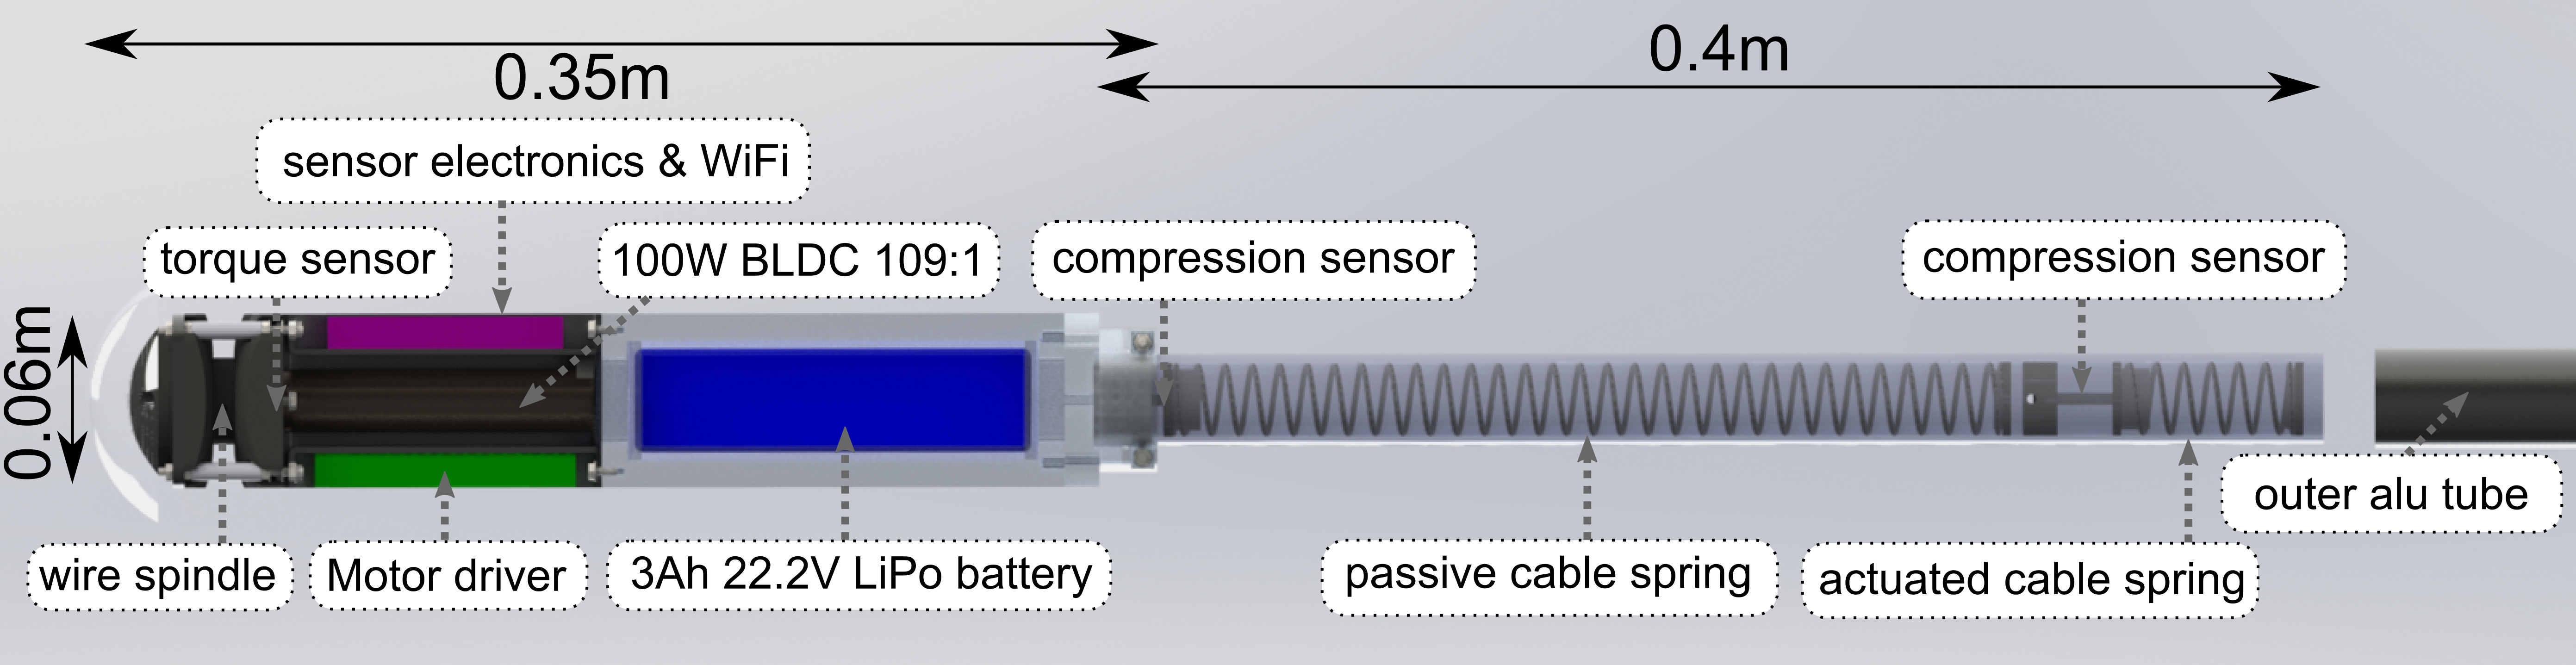
\includegraphics[width=0.9\columnwidth]{img/strut.png}
      \caption{Design v1.0 of a SUPERball endcap (and strut tube.) Note the four subsystems placed along the endcap, as well as the lack of detailed designs for mechanisms.}
      \label{fig:strutrender}
      \vspace{-0.2cm}
\end{figure}

Figure \ref{fig:strutrender} shows the very first version of SUPERball, denoted v1.0, for which detail design existed but was plagued with performance issues and which required more optimization~\cite{bruce2014design}.
This render comes from a that early CAD model, and though a hardware version of this rod was constructed, the imagery is less informative than the render.


\begin{figure}[thpb]
      \centering
      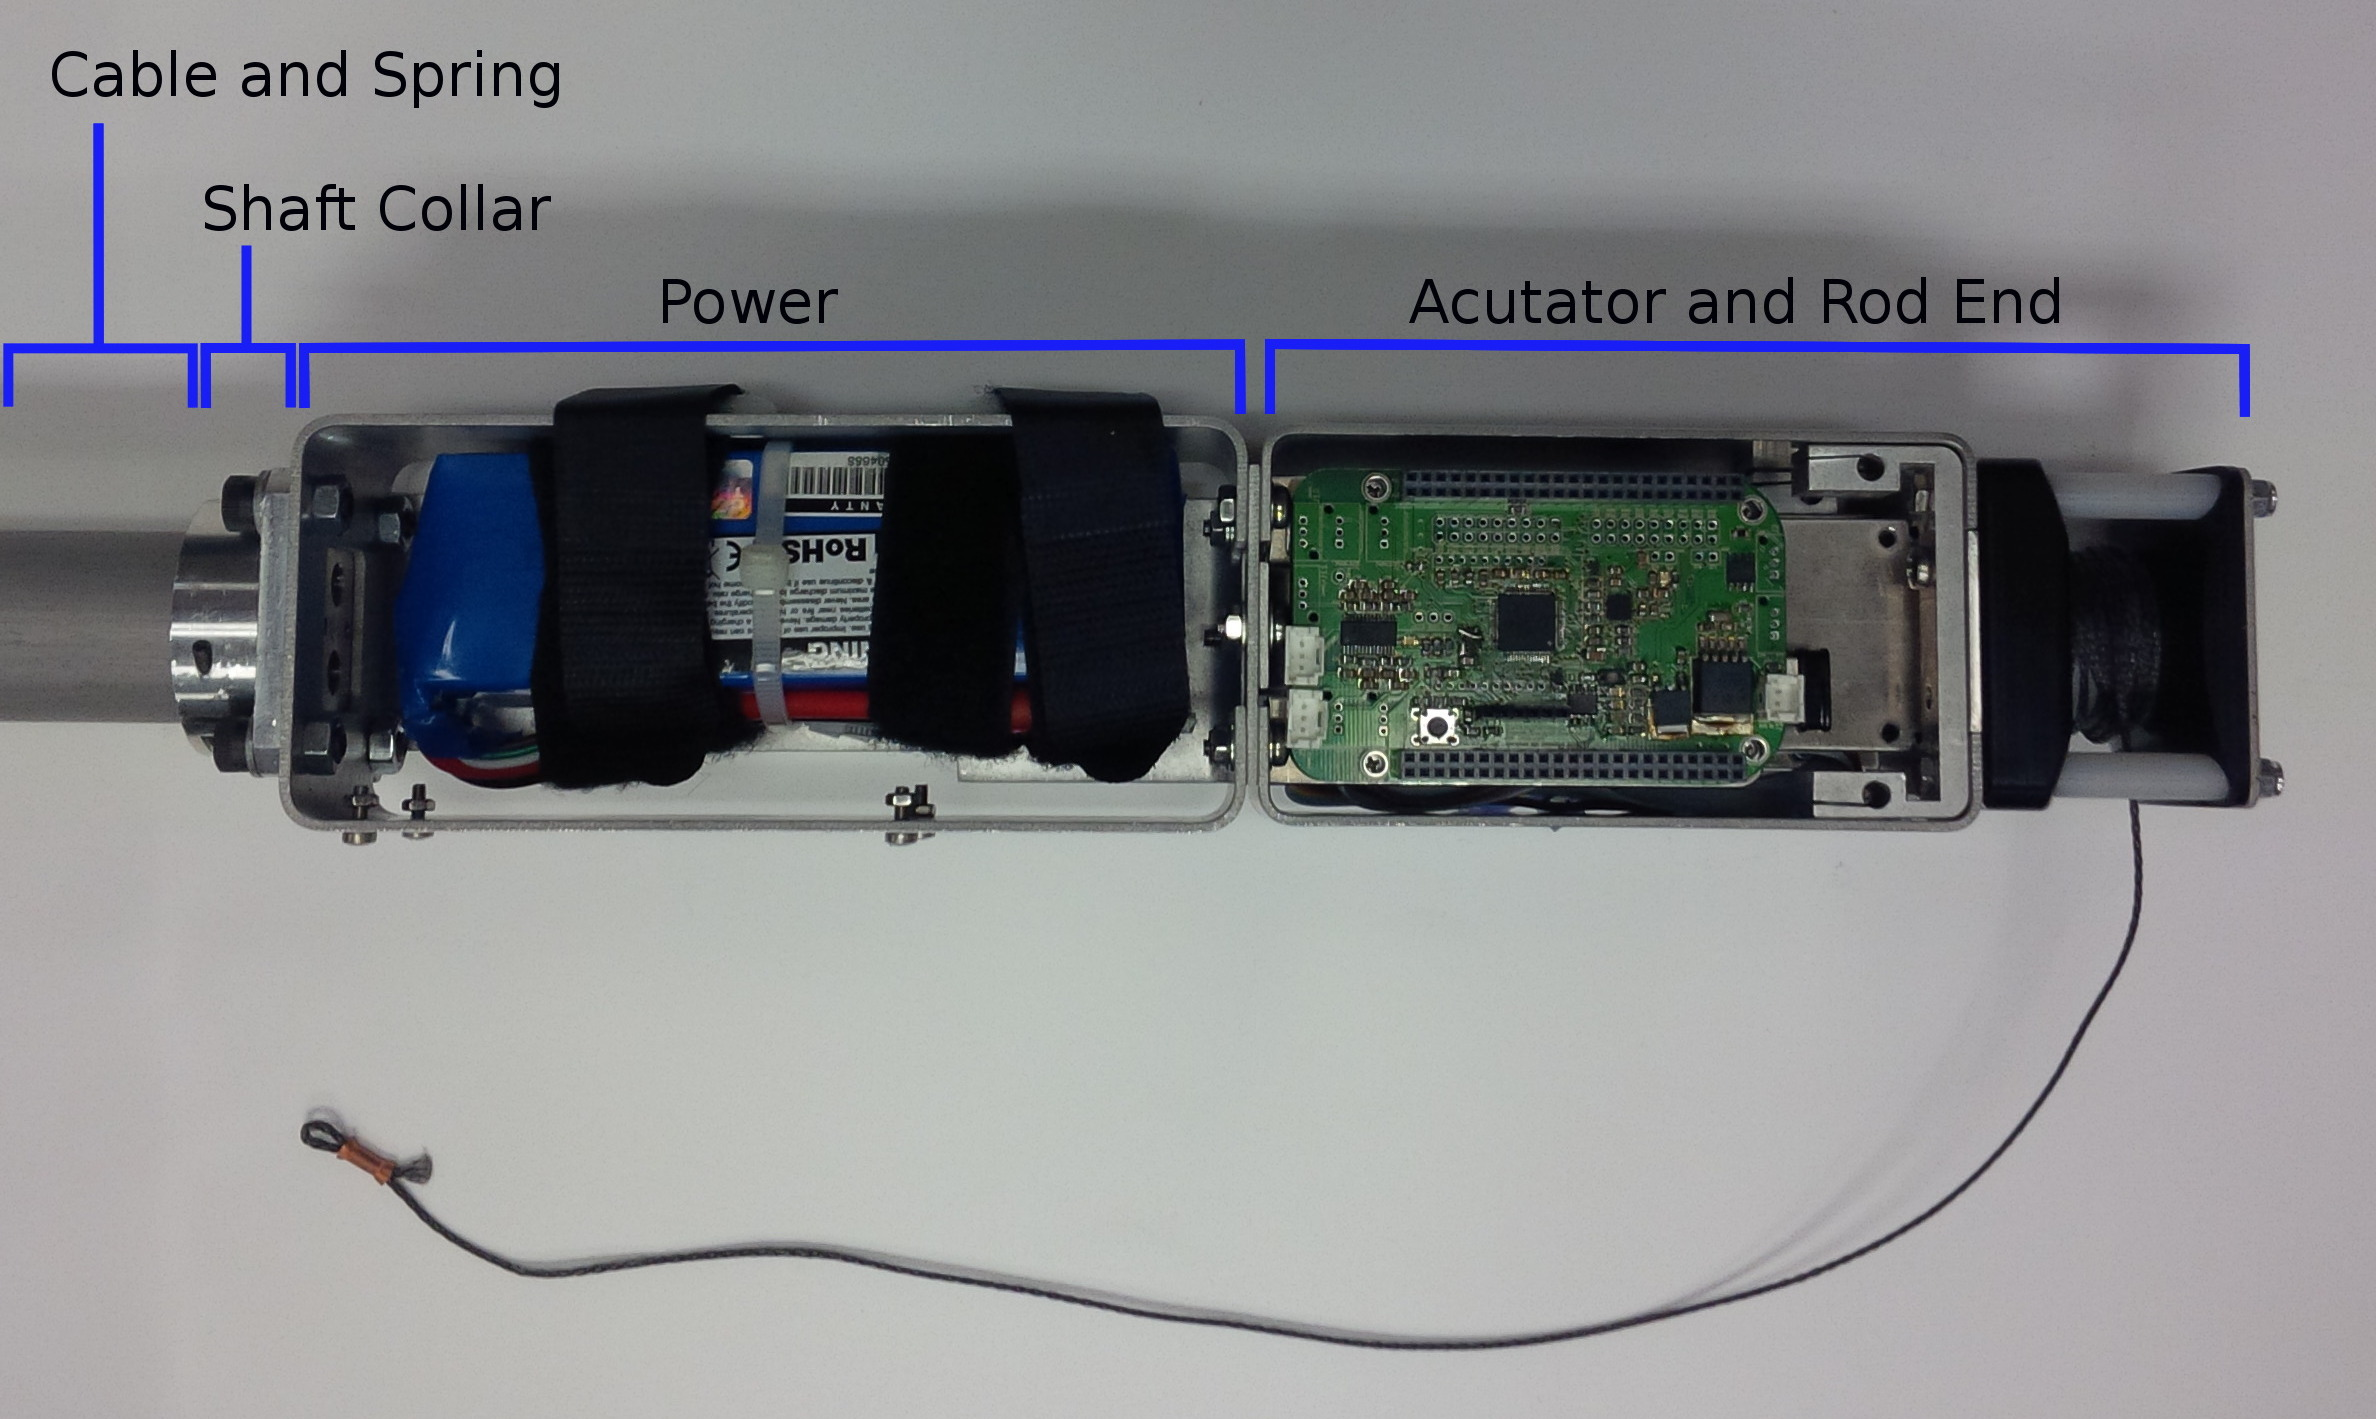
\includegraphics[width=0.9\columnwidth]{img/subsystem_end-cap_cropped.jpg}
      \caption{Version 1.5 prototype design of one of SUPERball's endcaps. Most structural components were implemented with sheet metal, and the actuator assembly includes updated mechanisms for the cable-spring system.}
      \label{fig:strut_prototype}
      \vspace{-0.2cm}
\end{figure}

In comparison, a heavily revised SUPERball endcap with finished detail design is shown in Figure \ref{fig:strut_prototype}.
This version is denoted v1.5, and was tested much more extensively.
The final version of the SUPERball rod, used on the full build-out of the prototype, is shown in Figures \ref{fig:final_endcap}.
This final version, v1.6, is that which is described in this report.
The overall configuration and purpose of each of these subassemblies was retained from the preliminary design to final prototype design.
However, as described in the sections below, the detail design phase for SUPERball led to many subtle improvements for these components and to multiple novel mechanisms and sensors.

\begin{figure}
  \centering
  \begin{subfigure}[b]{0.4\textwidth}
    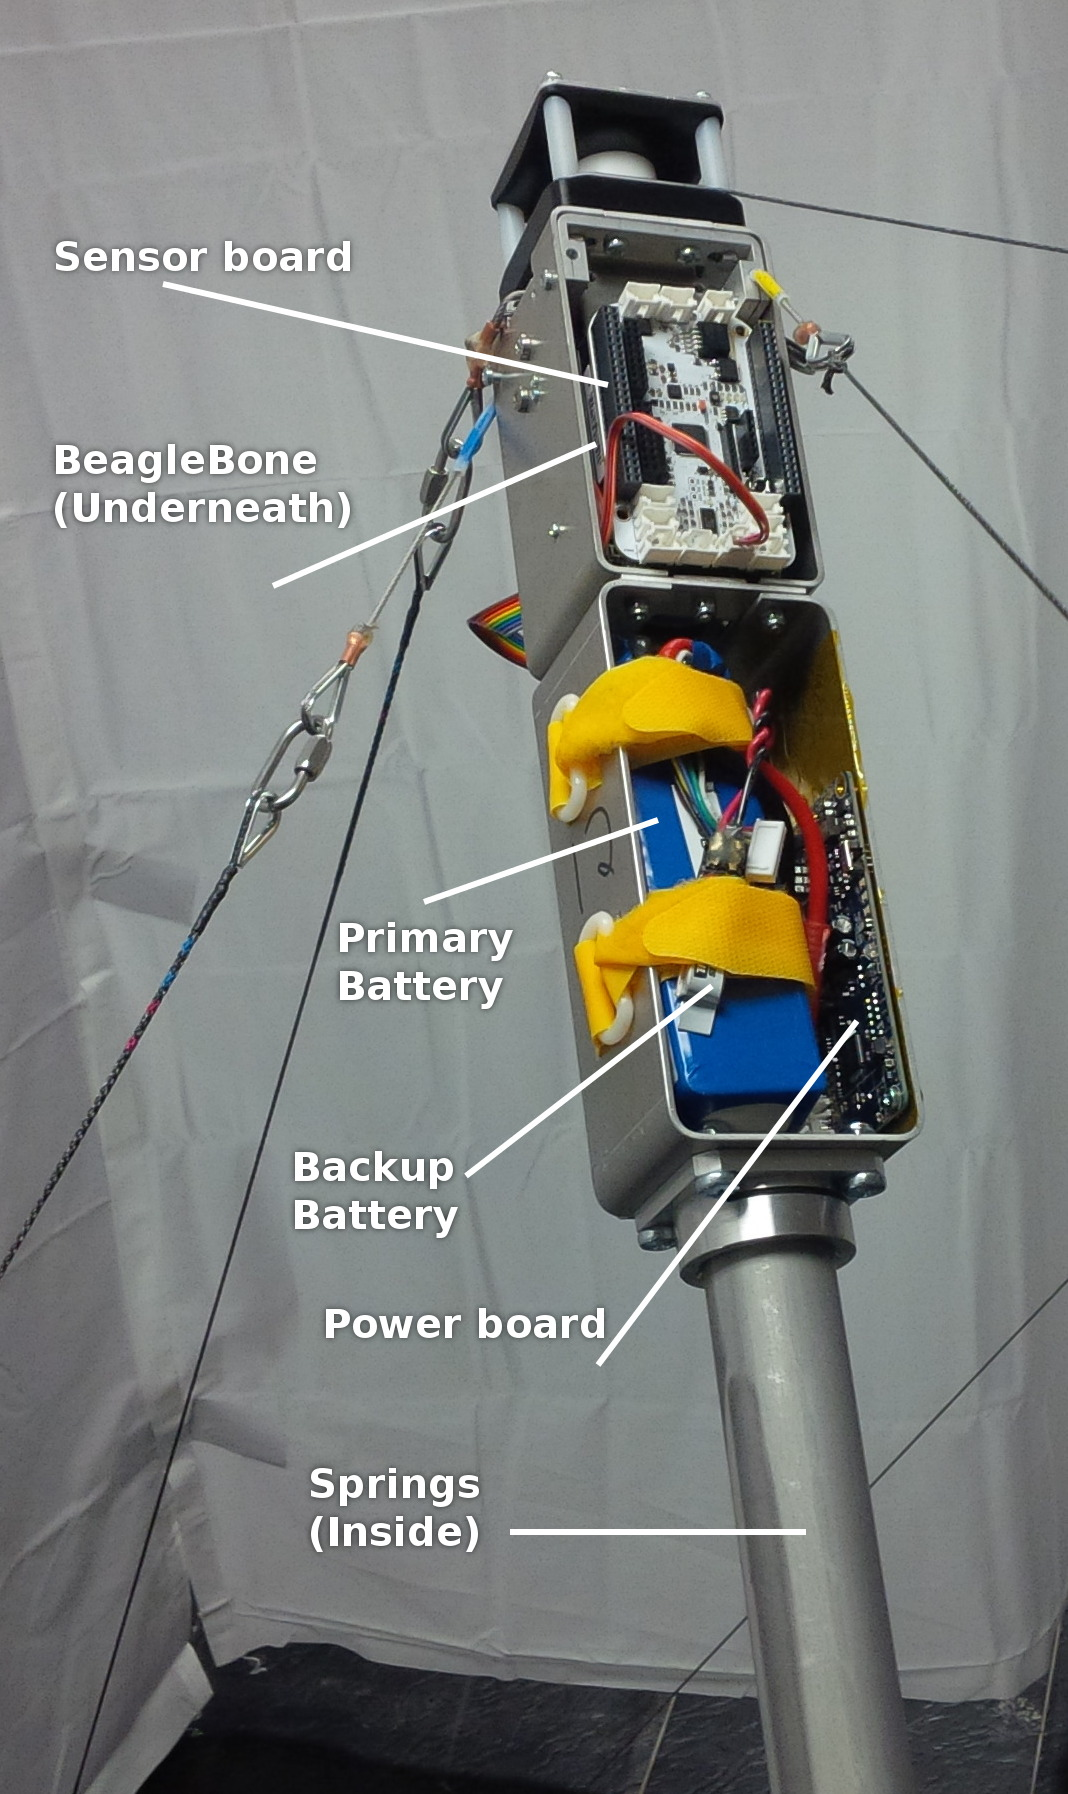
\includegraphics[width=1\textwidth]{img/endcap_upclose_sensorboard_labelled.jpg}
    \caption{Front side of the v1.6 endcap. The springs of the spring-cable assemblies are inside the hollow aluminum tube. Steel wire cable transfers motion from the springs to the outer cables, and is routed through the end cap assembly using various PTFE tubes and pulley-bearing elements.}
    \label{fig:final_endcap_front}
  \end{subfigure}
  \begin{subfigure}[b]{0.4\textwidth}
    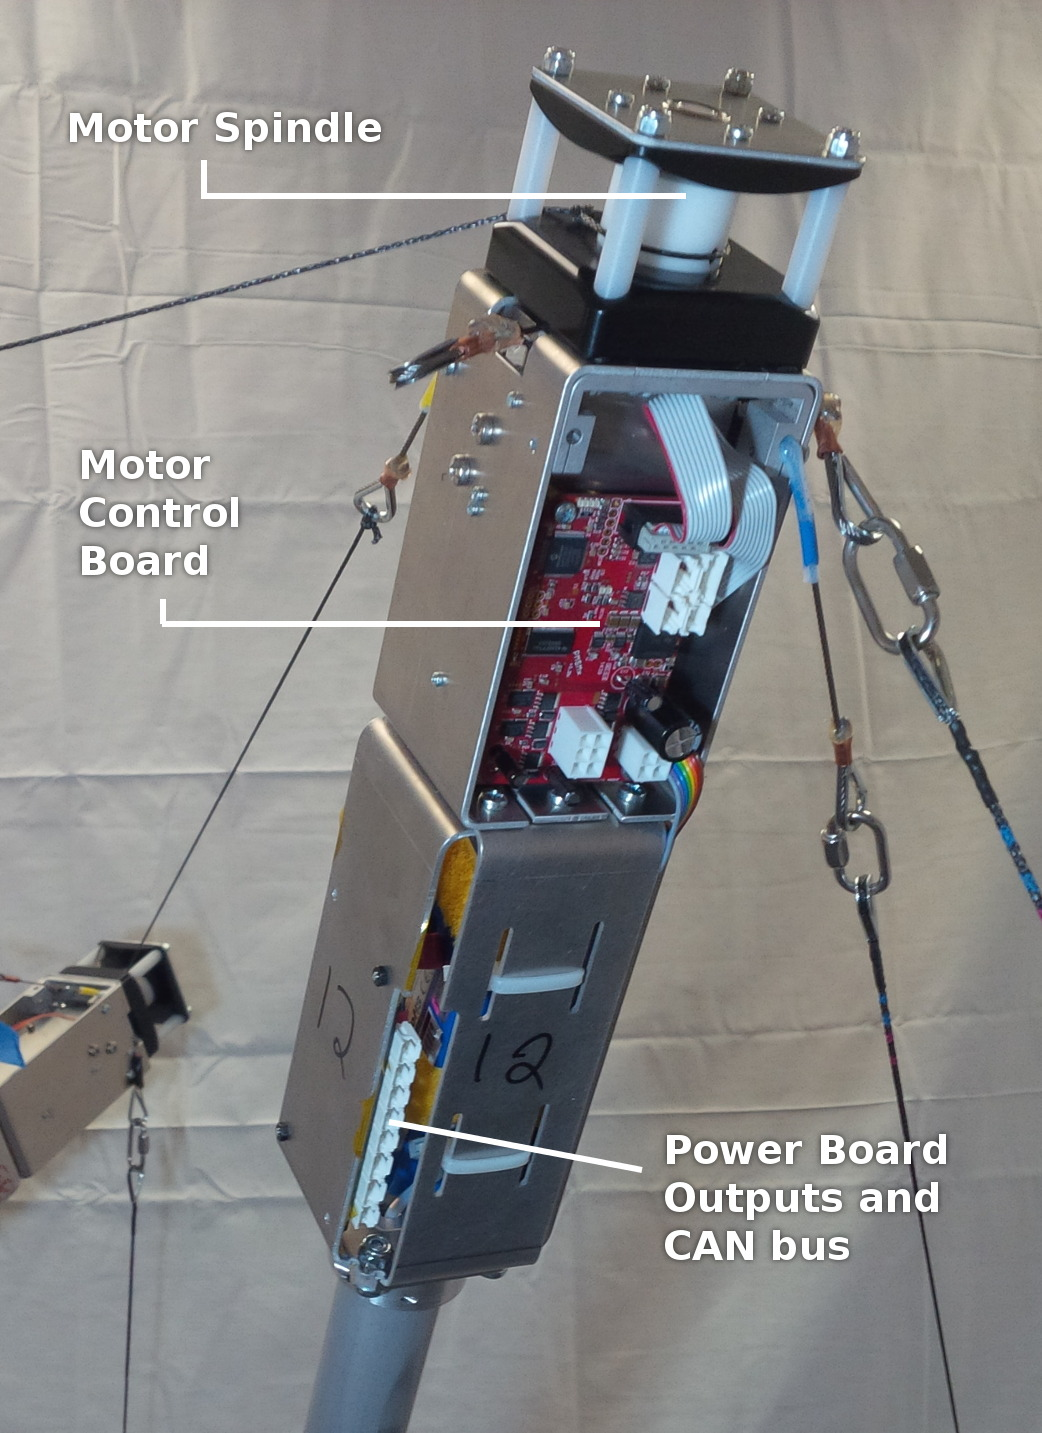
\includegraphics[width=1\textwidth]{img/endcap_upclose_motorboard_labelled.jpg}
    \caption{Reverse side of the v1.6 endcap. This side shows the other PCB for motor control, and a better view of the actuator assembly and spool caps.}
    \label{fig:final_endcap_reverse}
  \end{subfigure}
  \caption{Revision v1.6 of SUPERball's endcap.}
  \label{fig:final_endcap}
\end{figure}


\begin{wrapfigure}{R}{0.4\columnwidth}
      \centering
      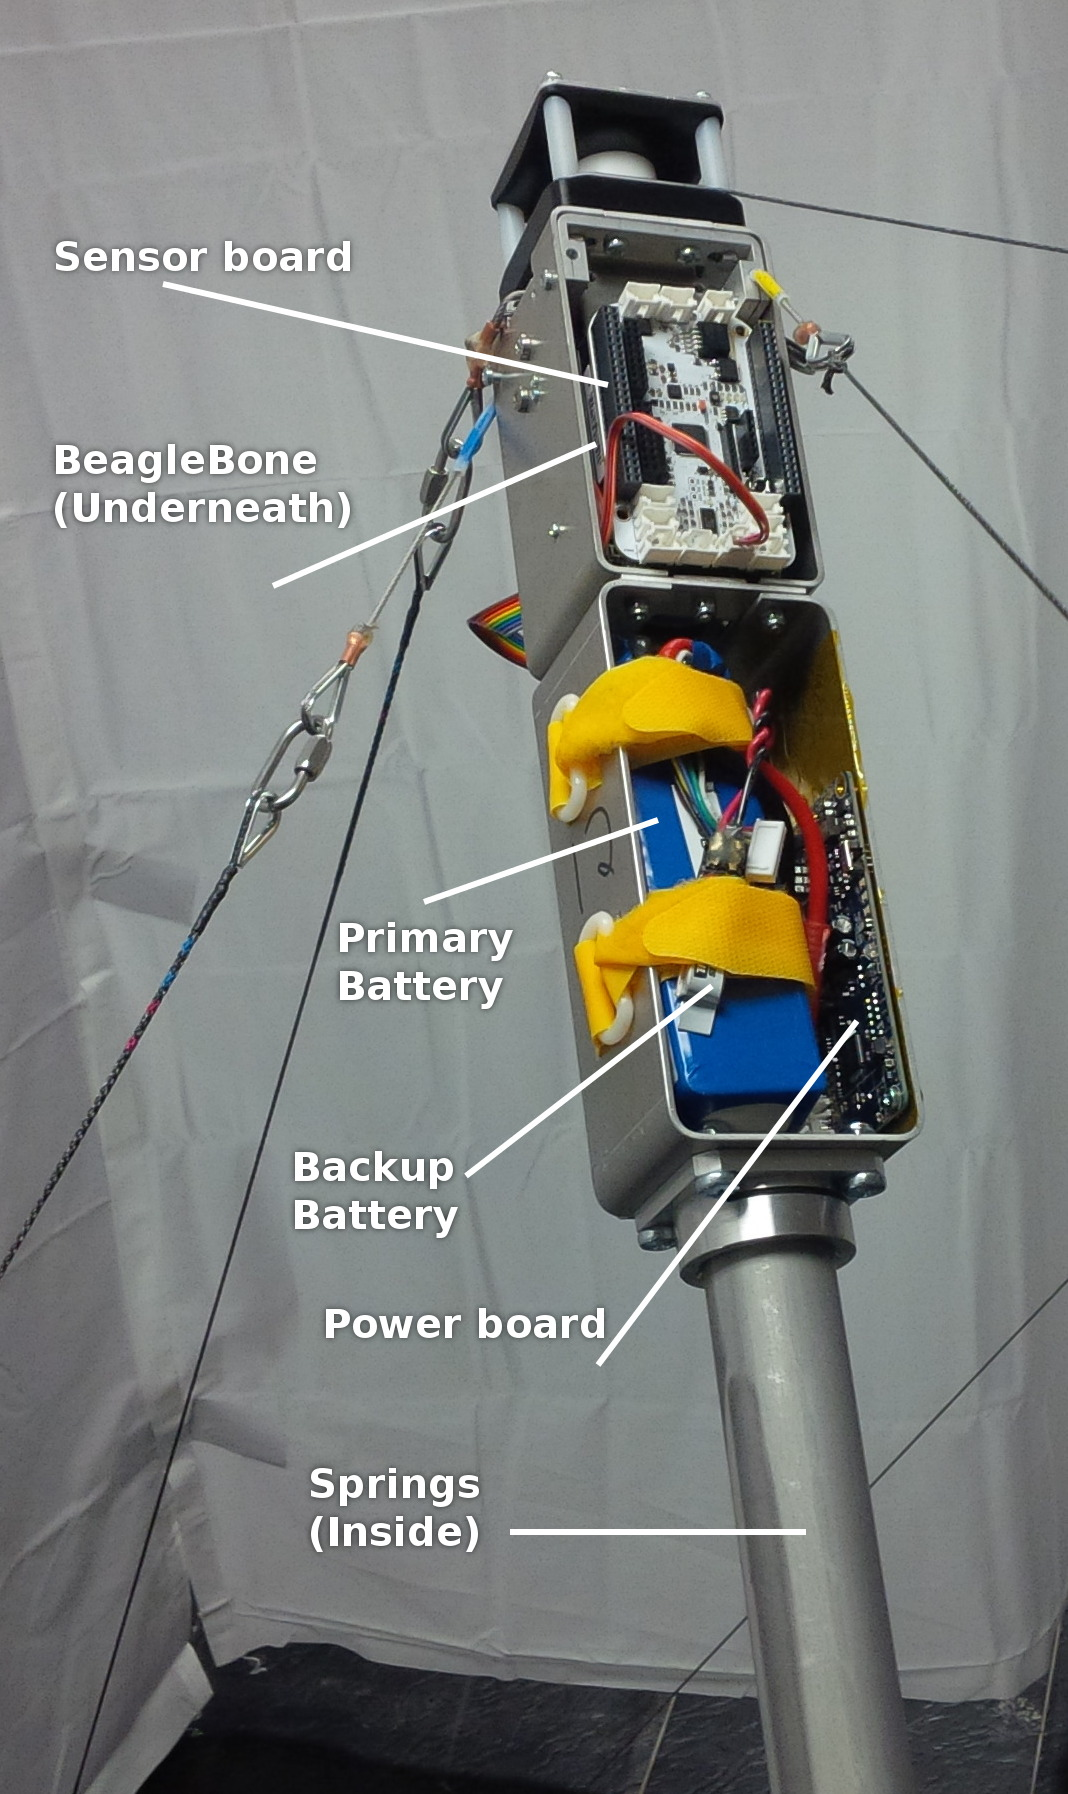
\includegraphics[width=.38\columnwidth]{img/endcap_upclose_sensorboard_labelled.jpg}
      \caption{One end cap of SUPERball, v1.6 final version. The springs of the spring-cable assemblies are inside the hollow aluminum tube. Steel wire cable transfers motion from the springs to the outer cables, and is routed through the end cap assembly using various PTFE tubes and pulley-bearing elements.}
      \label{fig:final_endcap}
      \vspace{-0.2cm}
\end{wrapfigure}

\section{Cable-Spring Subsystem}

In SUPERball, the tensile elements are called \emph{spring-cable assemblies} and consist of a combination of steel wire cable, Vectran cable, a compression spring, sensors and optionally an actuator.
Figure~\ref{fig:springcable} shows the conceptual model of such a system.
Each of SUPERball's motors is attached to a $1.4mm$-diameter Vectran cable (Cortland 7012 Vectran HT, $2.2kN$ breaking strength).
Sensors and actuators are discussed in later sections of this report.

\begin{figure}[thpb]
      \centering
      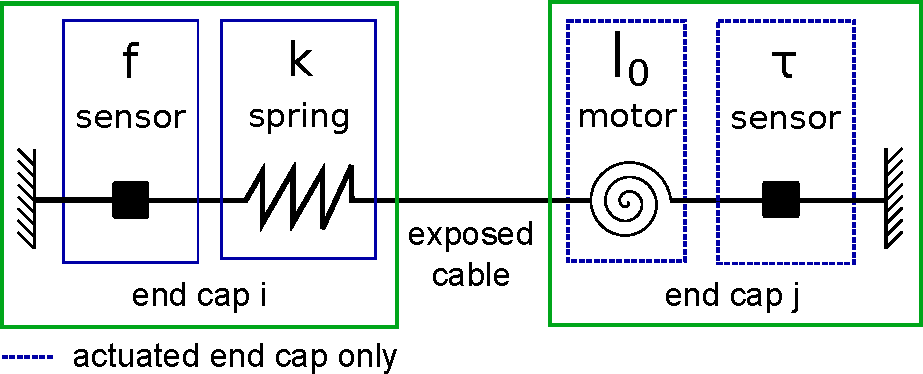
\includegraphics[width=.5\columnwidth]{img/spring_assembly.pdf}
      \caption{Conceptual model of a SUPERball spring-cable assembly. 
Each spring-cable assembly contains a (compression) spring with linear stiffness $k$. 
The current spring force or cable tension $f$ is measured by an in-line compressive force sensor.
Only the cables are exposed to the environment as all sensors and actuators are embedded in the end caps. 
The dashed elements - motor \& torque sensor - are available on actuated spring-cable assemblies.
Such assemblies are effectively series elastic actuators (SEA) with a significant amount of passive compliance.
The remote cable tension $f$ on end cap $i$ is only available to the motor controller on end cap $j$ through a wireless link.
Motor-side torque sensing $\tau$ allows for local tension control on end cap $j$, without introducing stringent requirements for the wireless link, which would reduce the flexibility of SUPERball's distributed design.
}
      \label{fig:springcable}
\end{figure}

The opposite end of that cable is looped onto the free end of a steel cable, close to the opposite rod, which then transfers force through the cable into a spring inside that other rod.
Figure~\ref{fig:cable_pulley_bearing_internals} shows the internals of the entrance point of this cable, which winds over a bearing then into a PTFE tube and then travels through the back of the end cap to the spring area.
Unactuated (passive) cables are attached directly to one end cap and to a compression spring and sensor inside another end cap.

\begin{figure}[thpb]
      \centering
      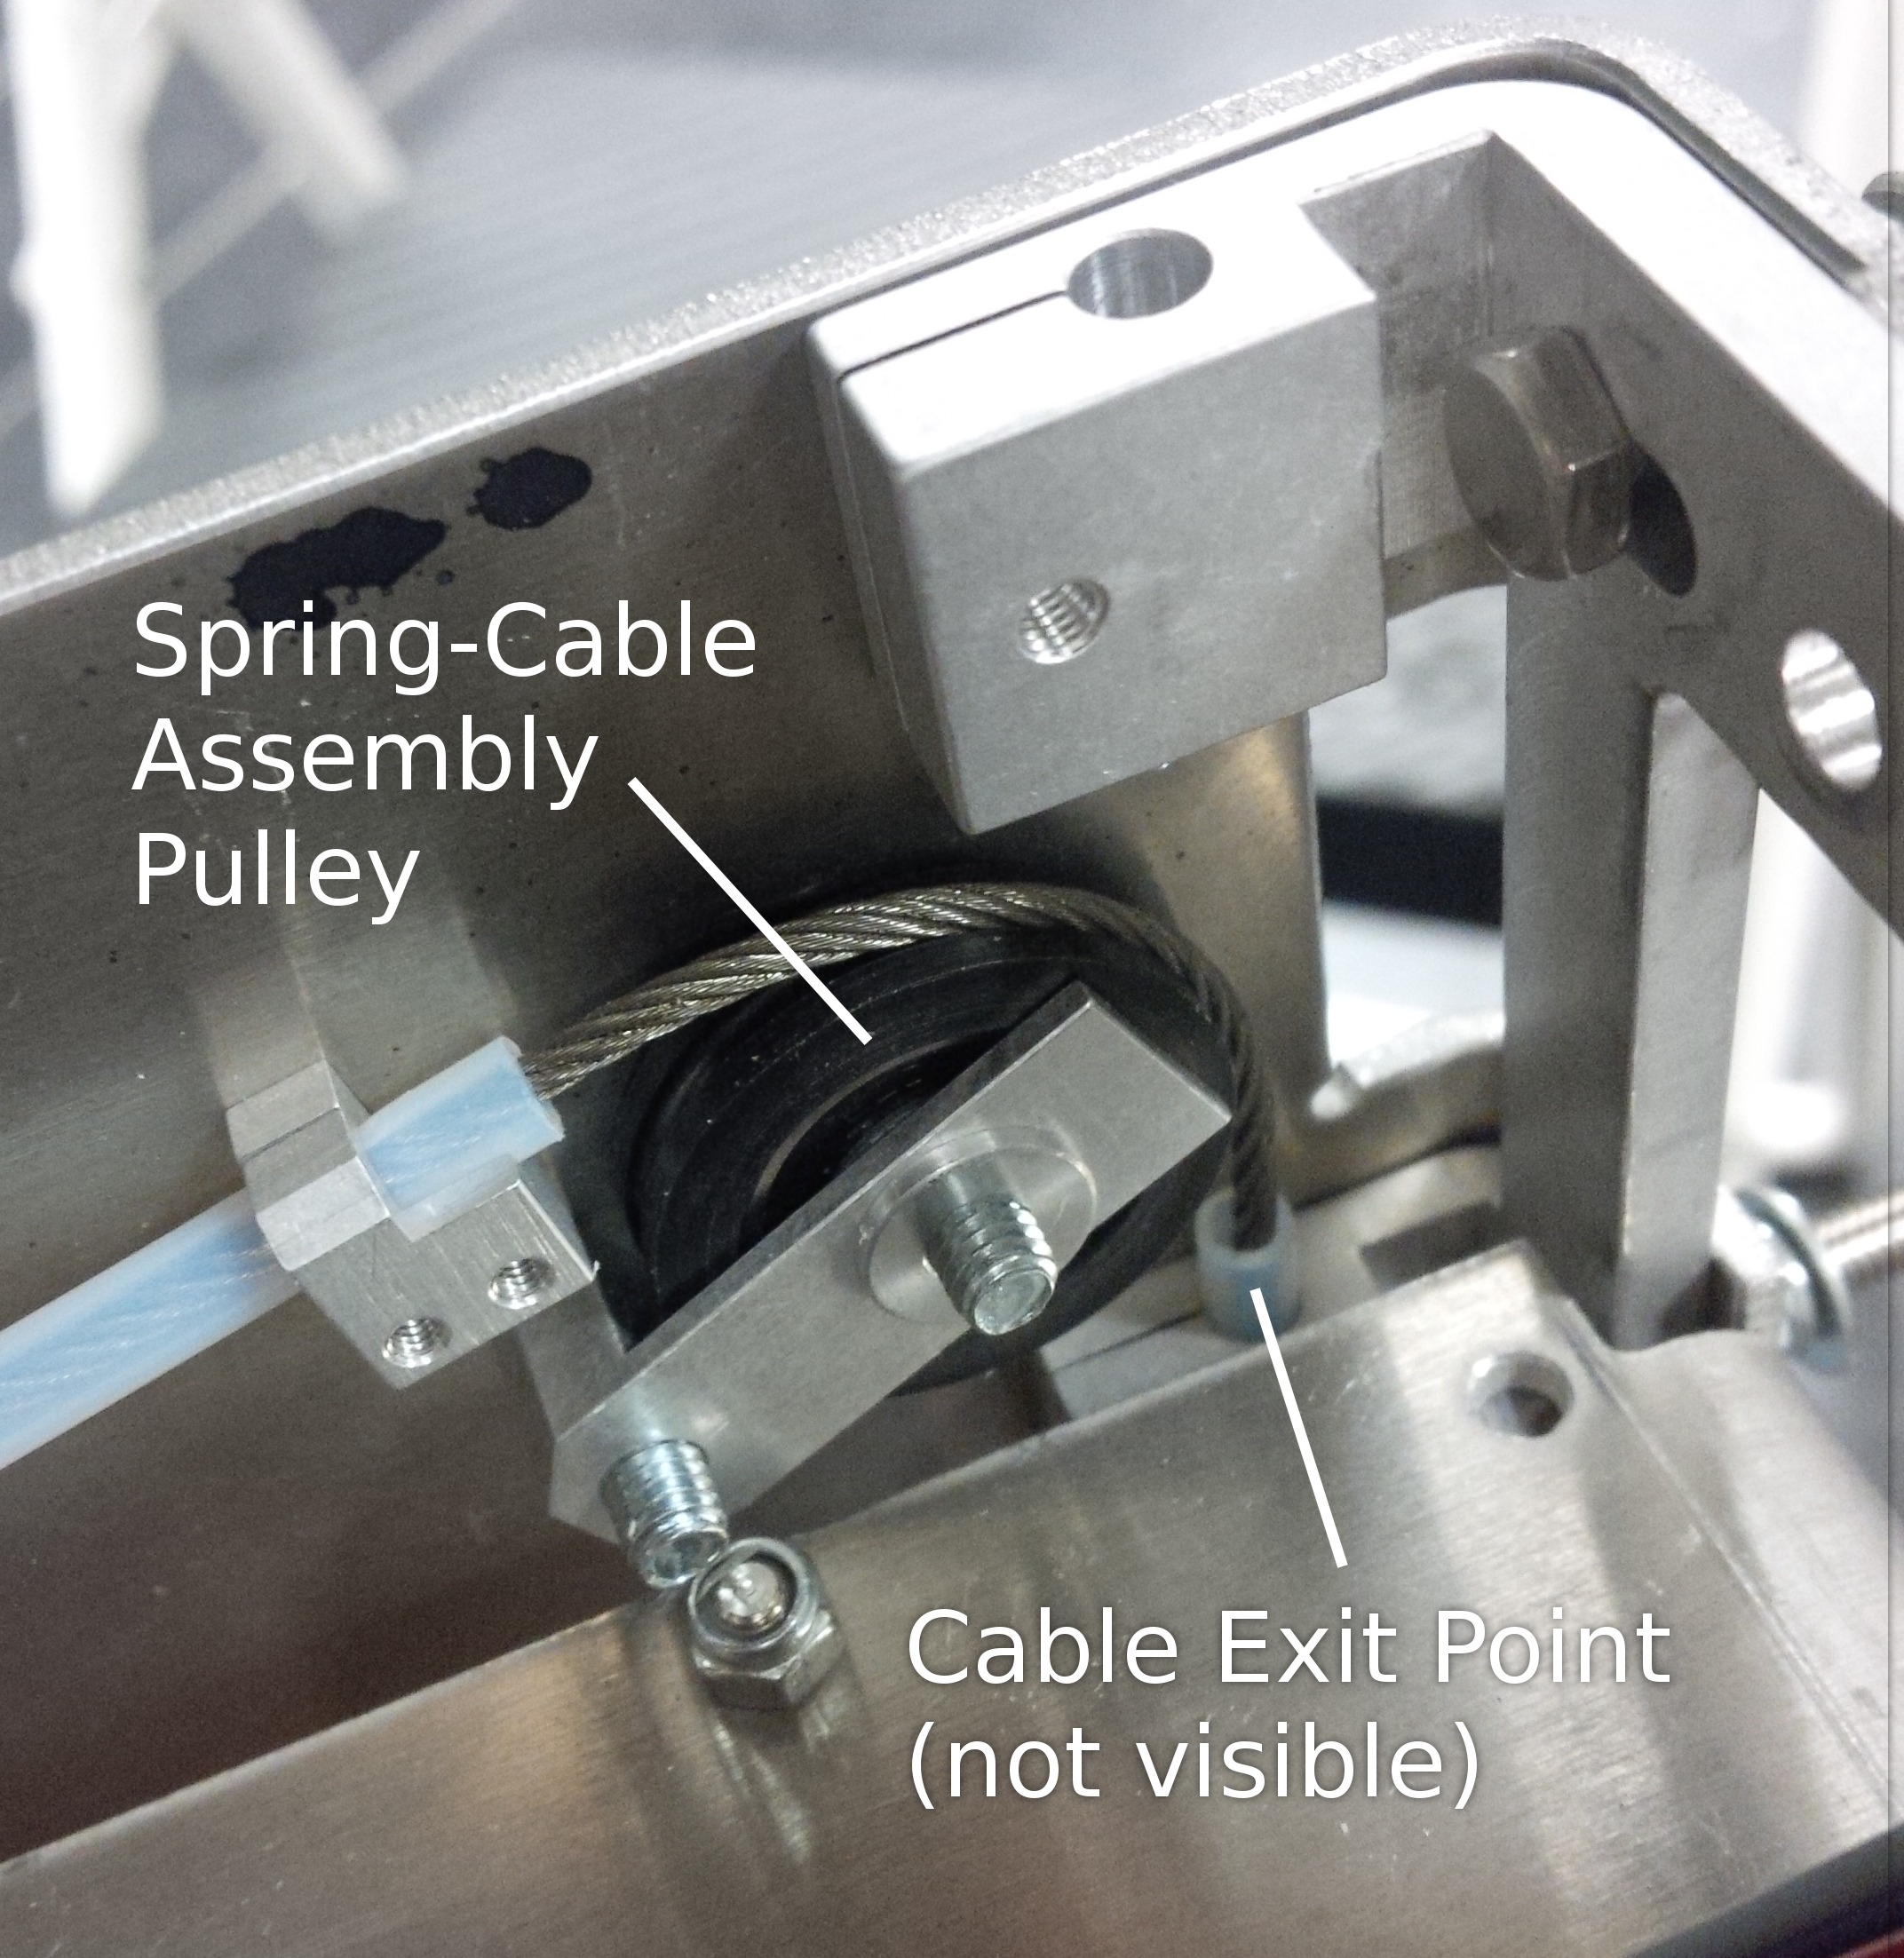
\includegraphics[width=.5\columnwidth]{img/cable_pulley_bearing_labelled.jpg}
      \caption{Internal view of the pulley and exit point of the steel cable, which connects to springs inside the strut tube on one end and to the external vectran cables on the other.}
      \label{fig:cable_pulley_bearing_internals}
      \vspace{-0.2cm}
\end{figure}

Since SUPERball is designed as a prototype on which to develop controls, a good model of the system was crucial - this led to the use of mechanical, metal springs for the cable's compliance over other materials with less deterministic spring constants (e.g. parachute cord.) 
On the modular end cap for SUPERball, an enclosed compression spring system was developed to alleviate issues observed in prior work~\cite{Caluwaerts2013rsif,bruce2014design} related to exposed extension springs.
Compression springs were chosen so that during any unknown impact, the springs would not plastically deform: at maximum force, the springs would simply bottom out, and thus SUPERball's states can be modelled as a hybrid system (compliant dynamics for one range of forces, direct force transfer into the endcaps for higher ranges of forces.) 
For SUPERball, a spring with a spring constant of $613 N/m$ is attached to a passive cable element and a $2850 N/m$ spring is attached to an actuated cable.
The passive spring has a much higher compressive range to allow for pretension to be instated into the passive springs. 

\begin{figure}[thpb]
      \centering
      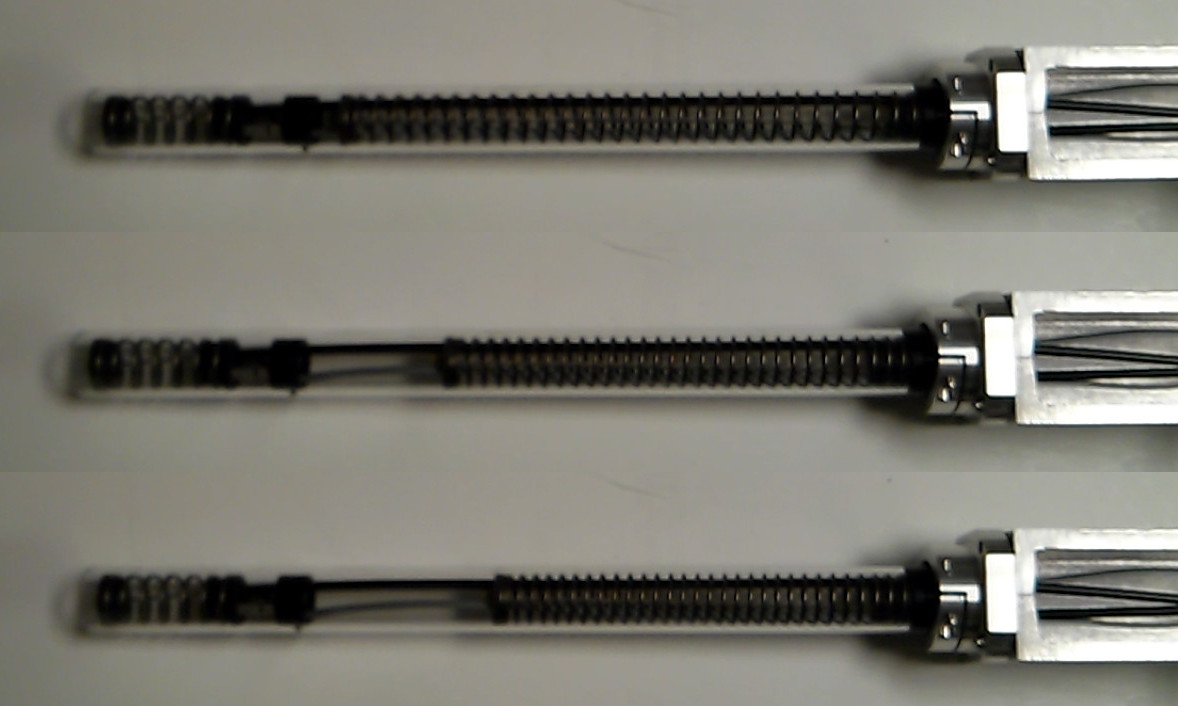
\includegraphics[width=.5\columnwidth]{img/double_spring_series_6-9-14.jpg}
      \caption{Compression spring movement on v1.0 of a SUPERball rod. This motion is largely unchanged in later versions, though the cable routing has been updated significantly as described above.}
      \label{fig:spring_series}
      \vspace{-0.2cm}
\end{figure}

An early working prototype of our spring holder system can be seen in Fig. \ref{fig:spring_series}, which demonstrates the compression of these springs.
See recent videos for~\cite{sabelhaus2015system} to see the most recent version of these springs in action.

\section{Rod Attachment (Shaft Collar)}

A critical aspect of SUPERball is the ability to exchange end-caps relatively quickly.
This is achieved by utilizing a simple shaft collar that clamps all the other subsystems to the connecting strut tube.
Since this collar is the only mounting component of the end-cap, it needs to be robust to loading forces yet simple for easy assembly.
The collar bolts onto both the battery compartment (and thereby the entire outer structure) as well as the internal cable-spring assembly.
It then clamps onto the outside of the strut tube through a friction-based shaft collar connection.
Figure \ref{fig:redesigned_shaft_collar} shows a perspective image of this component.

\begin{wrapfigure}{R}{0.45\columnwidth}
  \begin{center}
    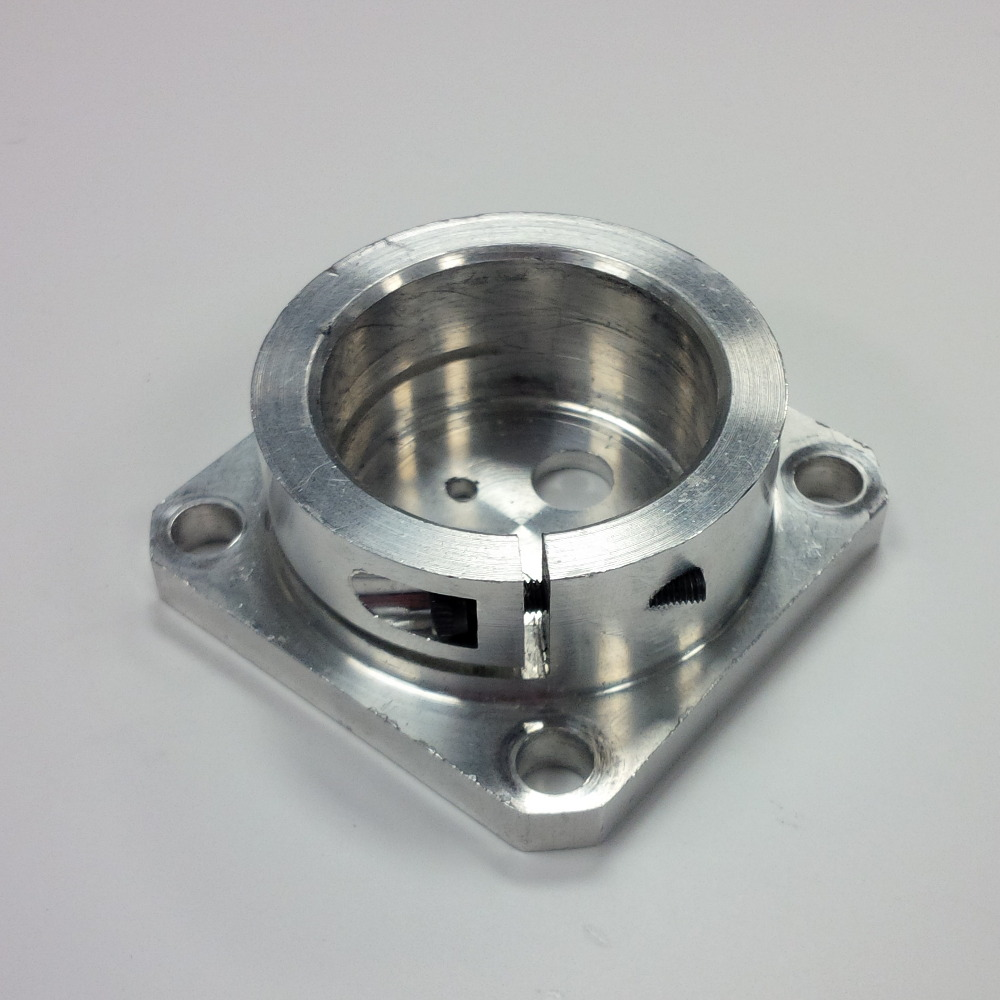
\includegraphics[width=0.33\textwidth]{img/redesigned_shaft_collar}
    \caption{Shaft collar mount for SUPERball.}
    \label{fig:redesigned_shaft_collar}
  \end{center}
%  \vspace{-0.5cm}
\end{wrapfigure}

Since this shaft collar is the heaviest manufactured part on SUPERball, it was optimized for reduced weight and ease of assembly/manufacturability through two specific features.
First, the collar was designed with only one screw (as opposed to a fully split collar), for ease of assembly in this tight press-fit, and which also eliminates a manufacturing step.
Then, the wall thicknesses and dimensions were optimized using a combination of rough hand calculations and FEA software (see section~\ref{sec:hardware_testing}) to ensure a reasonable safety factor while reducing its size and weight.

\section{Power Subsystem}

The power subsystem consists of three main sets of components: a large lithium polymer battery, a controller PCB, and the sheet metal structure to which it is all attached.

\begin{wrapfigure}{R}{0.45\columnwidth}
   \centering
   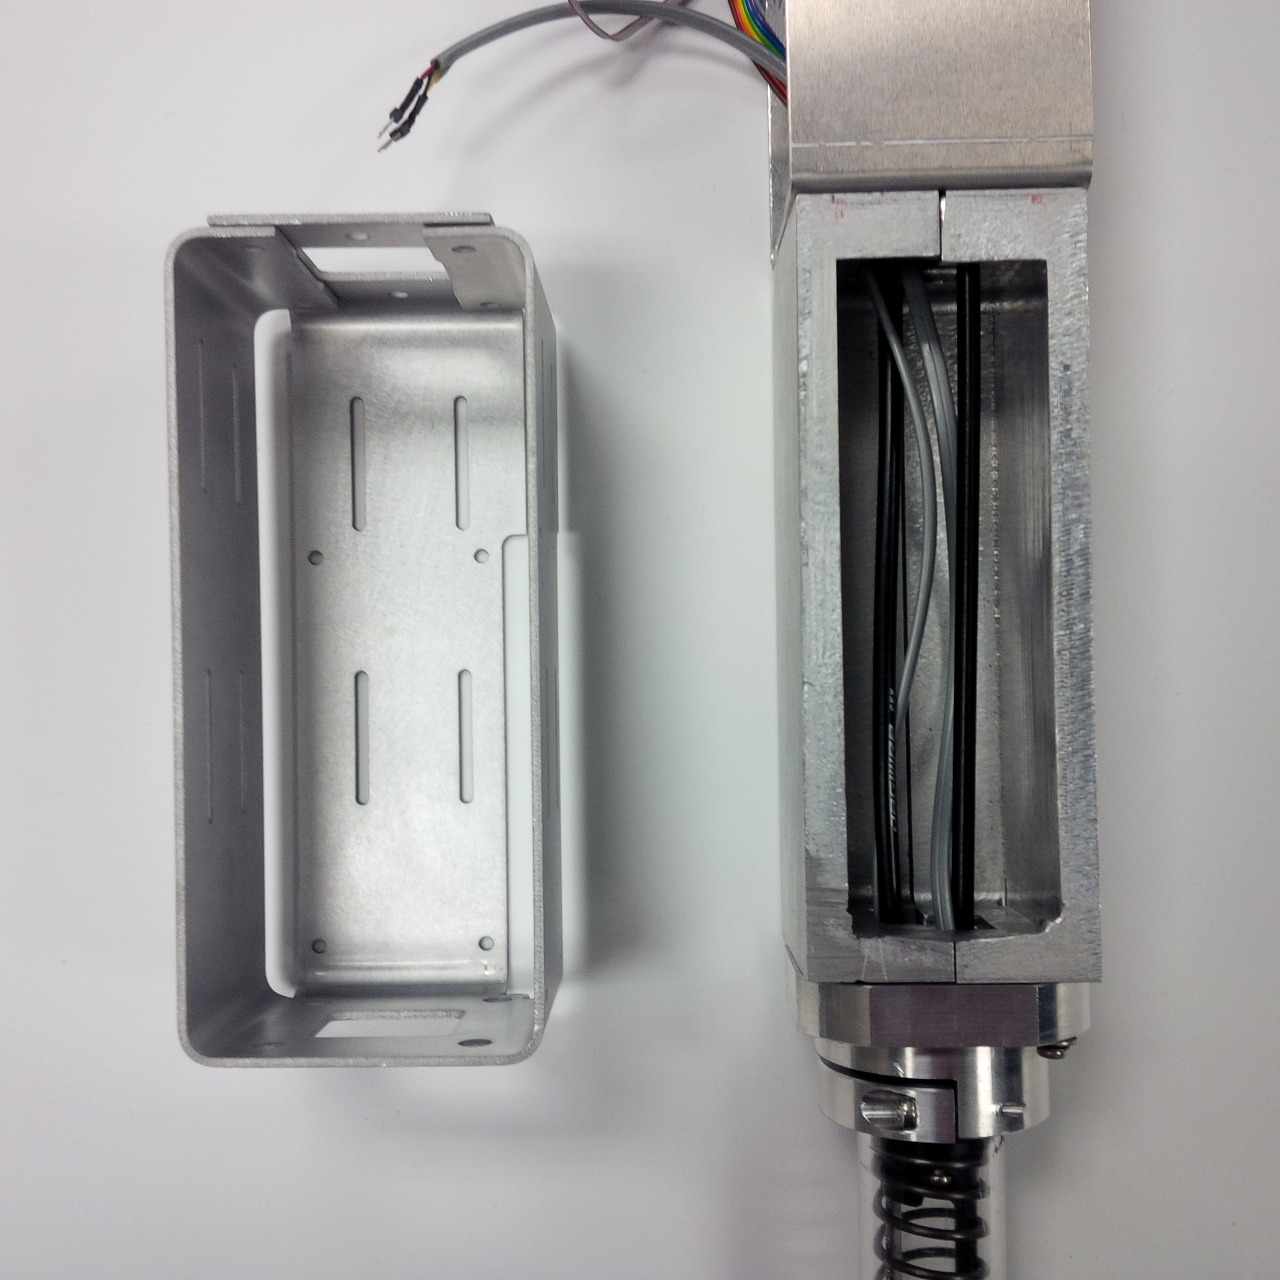
\includegraphics[width=0.45\columnwidth]{img/battery_compartment} 
   \caption{SUPERball's power subsystem structural housing (battery compartment.) Right: Original v1.0 design. Left: Redesigned compartment for v1.5 and 1.6.}
   \label{battery_compartment}
%%   \vspace{-0.5cm}
\end{wrapfigure}

As shown in Figure \ref{battery_compartment}, initial design (v1.0) of this subsystem used two pieces of bulk aluminum milled out to house the battery.
While this provided excellent structural support, multiple performance characteristics compelled a switch to a bent sheet metal aluminum design.
First, weight was reduced significantly. 
After initial calculations indicated over-designed dimensions and an enormous safety factor for this part, these wall thicknesses were reduced to the point at which they effectively became sheet metal.
Second, manufacturing became simpler: as opposed to a costly and complex CNC milling operation, this bracket could be cut from sheet with a water jet, then bent with a CNC sheet metal bender.
Finally, more flexibility was required for placement of components.

Initial designs of placement of the large 3 Amp-hour battery compelled the need for dedicated tie-down straps, in order to facilitate exact placement of the component as well as allow for ease of replacing drained batteries.
Thus, holes were needed for straps, shown in above pictures holding the battery to the side of the compartment.

In addition, systems-level design indicated the need for a discrete power management controller.
A logical placement is physically close to the battery, which required more room than existed in the initial bulk design.
The final version in Figure \ref{battery_compartment} shows multiple mounting holes for standoffs for such a printed circuit board, as well as slots for different straps to secure the battery as needed.
It consists of five bends which fold together at the top section, and are then compressed together by the same bolt patter which attaches the compartment to the sheet metal surrounding the motor.

Sheet metal designs in the first iteration of SUPERball showed some microcracks from harsh bending angles.
Thus, this battery compartment was designed to account for gentler bend radii.
Each of these bends was designed with a radius of three times the the sheet thickness, or 6mm.
These same radii were used in the most recent version of the sheet metal brackets that support the motor and actuation subsystem.

\section{Actuation Subsystem}
The actuation subsystem is designed for ease of assembly and manufacturing, as well as to further reduce friction in the motor-driven cable.
Figure~\ref{actuation_open_view} displays the motor assembly, 
which at its core is similar to the one present on SUPERball's predecessor, ReCTeR~\cite{Caluwaerts2013rsif}.
However, the new design is significantly more robust and versatile.

\begin{wrapfigure}{R}{0.33\columnwidth}
   \centering
   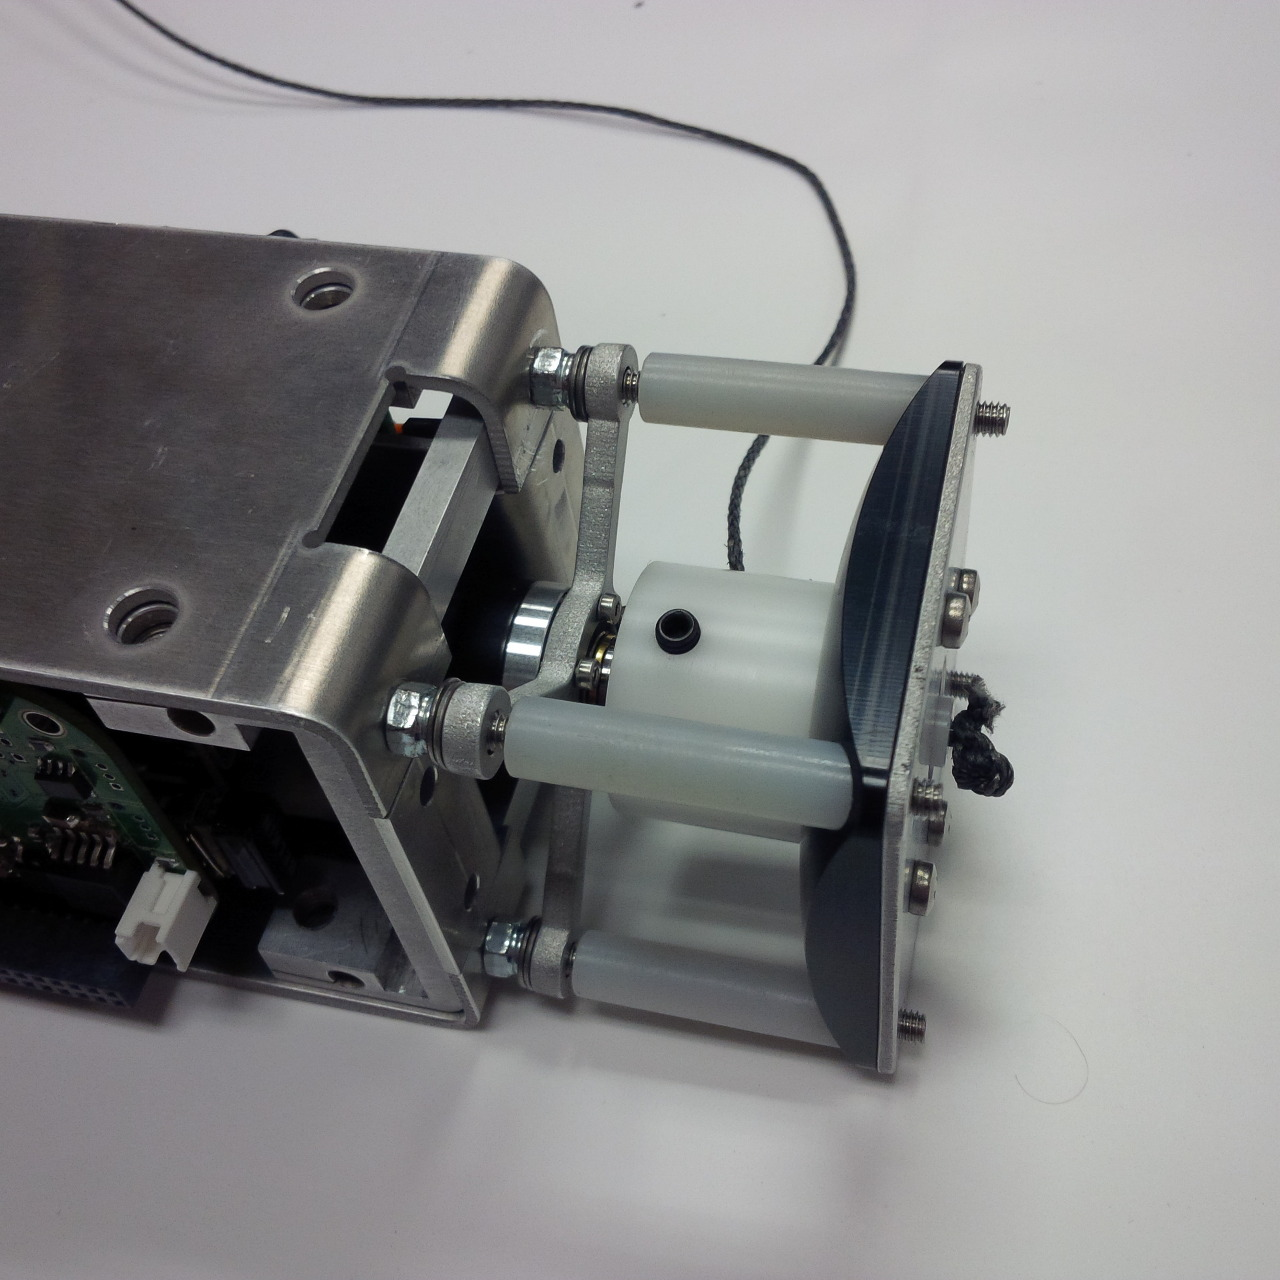
\includegraphics[width=0.33\columnwidth]{img/actuation.jpg} 
   \caption{Actuator design with bottom spool cap removed and exposed motor torque sensor. 
A POM spindle mounted onto the motor axis actuates a Vectran cable. 
This open construction exposes the wire and spindle, but reduces the cable friction and risk of knots.
The design is shown without protective rubber cap.}
   \label{actuation_open_view}
%%   \vspace{-0.5cm}
\end{wrapfigure}

The simple, yet robust design of the cable actuator is based on a spindle actuated by a geared brushless DC motor.
The motor axis is secured by two radial bearings, one  of which is press fitted into the plate on top of the spindle and one is integrated into the gear box.
A spindle (30mm diameter) machined out of POM sits on top of the motor axis and winds up the aforementioned Vectran cable.
Vectran cable has lower creep than Dyneema which was used on the previous prototype robot, 
but without protective coating it is sensitive to UV light~\cite{fette2004vectran}~\cite{said2006investigation}.
It has been successfully used in space applications (e.g., the Mars Pathfinder airbags) due to its excellent thermal properties.

\begin{wrapfigure}{l}{0.33\columnwidth}
   \centering
   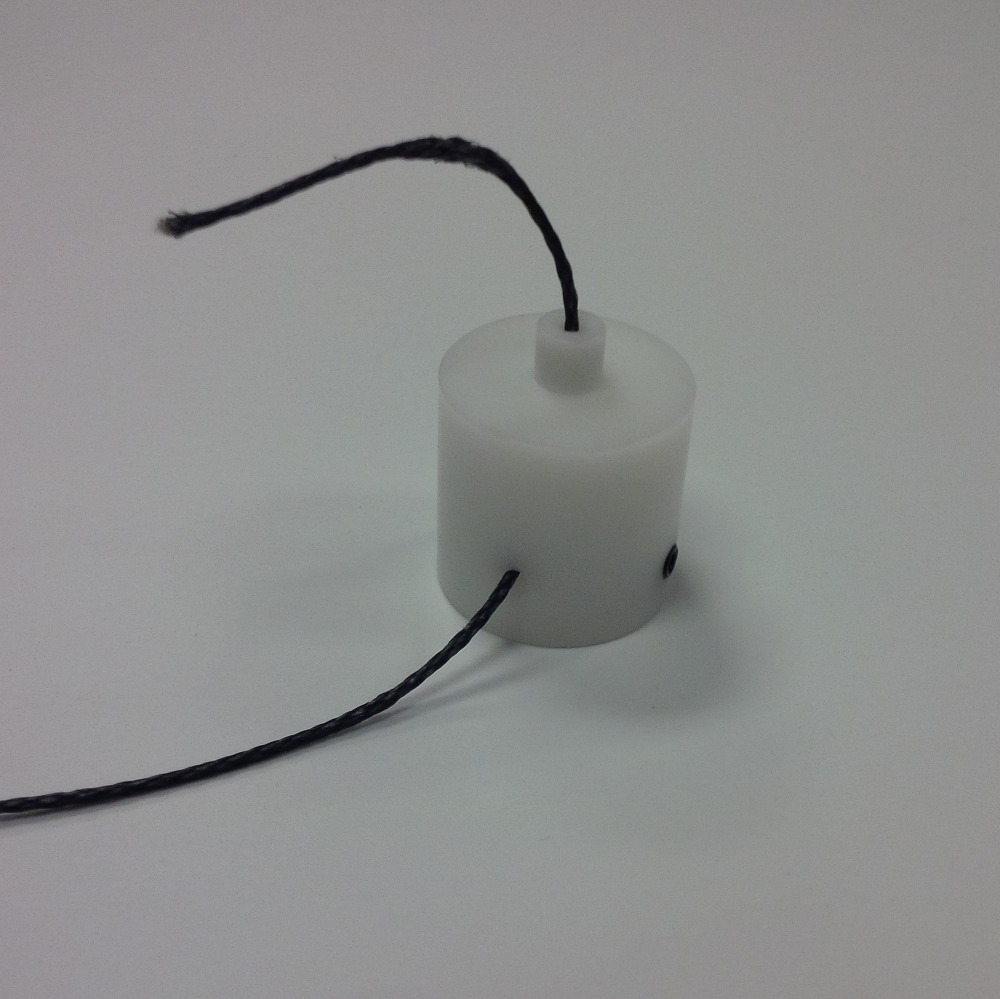
\includegraphics[width=0.33\columnwidth]{img/spindle} 
   \caption{Spindle with Vectran cable.}
   \label{spindle_pic}
%%   \vspace{-0.5cm}
\end{wrapfigure}

The motor spindle has a guide passageway for the cable to pass through it, 
from the side to the top of the assembly (underneath any future protective rubber covering for the top).
The cable is designed to slide into the spindle from the slide and come out on top of the assembly.
This allows safe clamping of the cable without damaging it.
Our NASA team studied various ways in which we can secure the one end of the Vectran cable that terminates underneath the rubber cap with minimal reduction of the breaking strength of the cable.
The most promising option embeds a steel ball inside the cable and then pots that section of the cable in epoxy.
Figure \ref{spindle_pic} shows this spindle with cable threaded through its guideway.
Work is ongoing to properly characterize this connection method.


It is important to prevent tight bends (knots) of the cable, as this reduces its strength and increases wear.
To further protect the cable and prevent it from getting stuck, the spindle is embedded into two smooth POM surfaces (spool caps), 
with a 0.5mm gap between the spindle and the surfaces.
This allows the cable to slide smoothly in almost any direction without excessive friction.

The bottom spool cap is designed to take all the force from the upper components (nylon spacers and top plate, screwed on with one nut at the top) and transmit it directly to the metal housing of the actuator assembly.
Note how the flanges take the load from the nylon spacers, which are loaded from the top plate, instead of the motor mount piece itself.
See section \ref{hardware_testing} for an analysis of the forces in these parts.

\section{Sensor Design}

SUPERball has three types of sensors: motor encoders, and two custom force/torque sensors constructed with strain gauges.
The following sections describe the two custom parts that together allow for state estimation of the robot (both centralized and distributed), though such estimation methods have yet to be implemented.

\subsection{Compressive Force Sensor}

Sensing the tensions of each of SUPERball's cables can be done by detecting the force transmitted from each of the compression springs to the spring housing.
This is an intuitively simple task that was complicated by the geometric constraints imposed by the cables that are routed back through the springs.
Since force was transmitted to the springs by a small press-fit cap with a notch for a steel cable, that cable needed to run back through the center of the spring.
Consequently, two thick cables needed to fit past the compressive force sensor, requiring a slim design with a small cross-sectional footprint.

\begin{figure}[thpb]
      \centering
      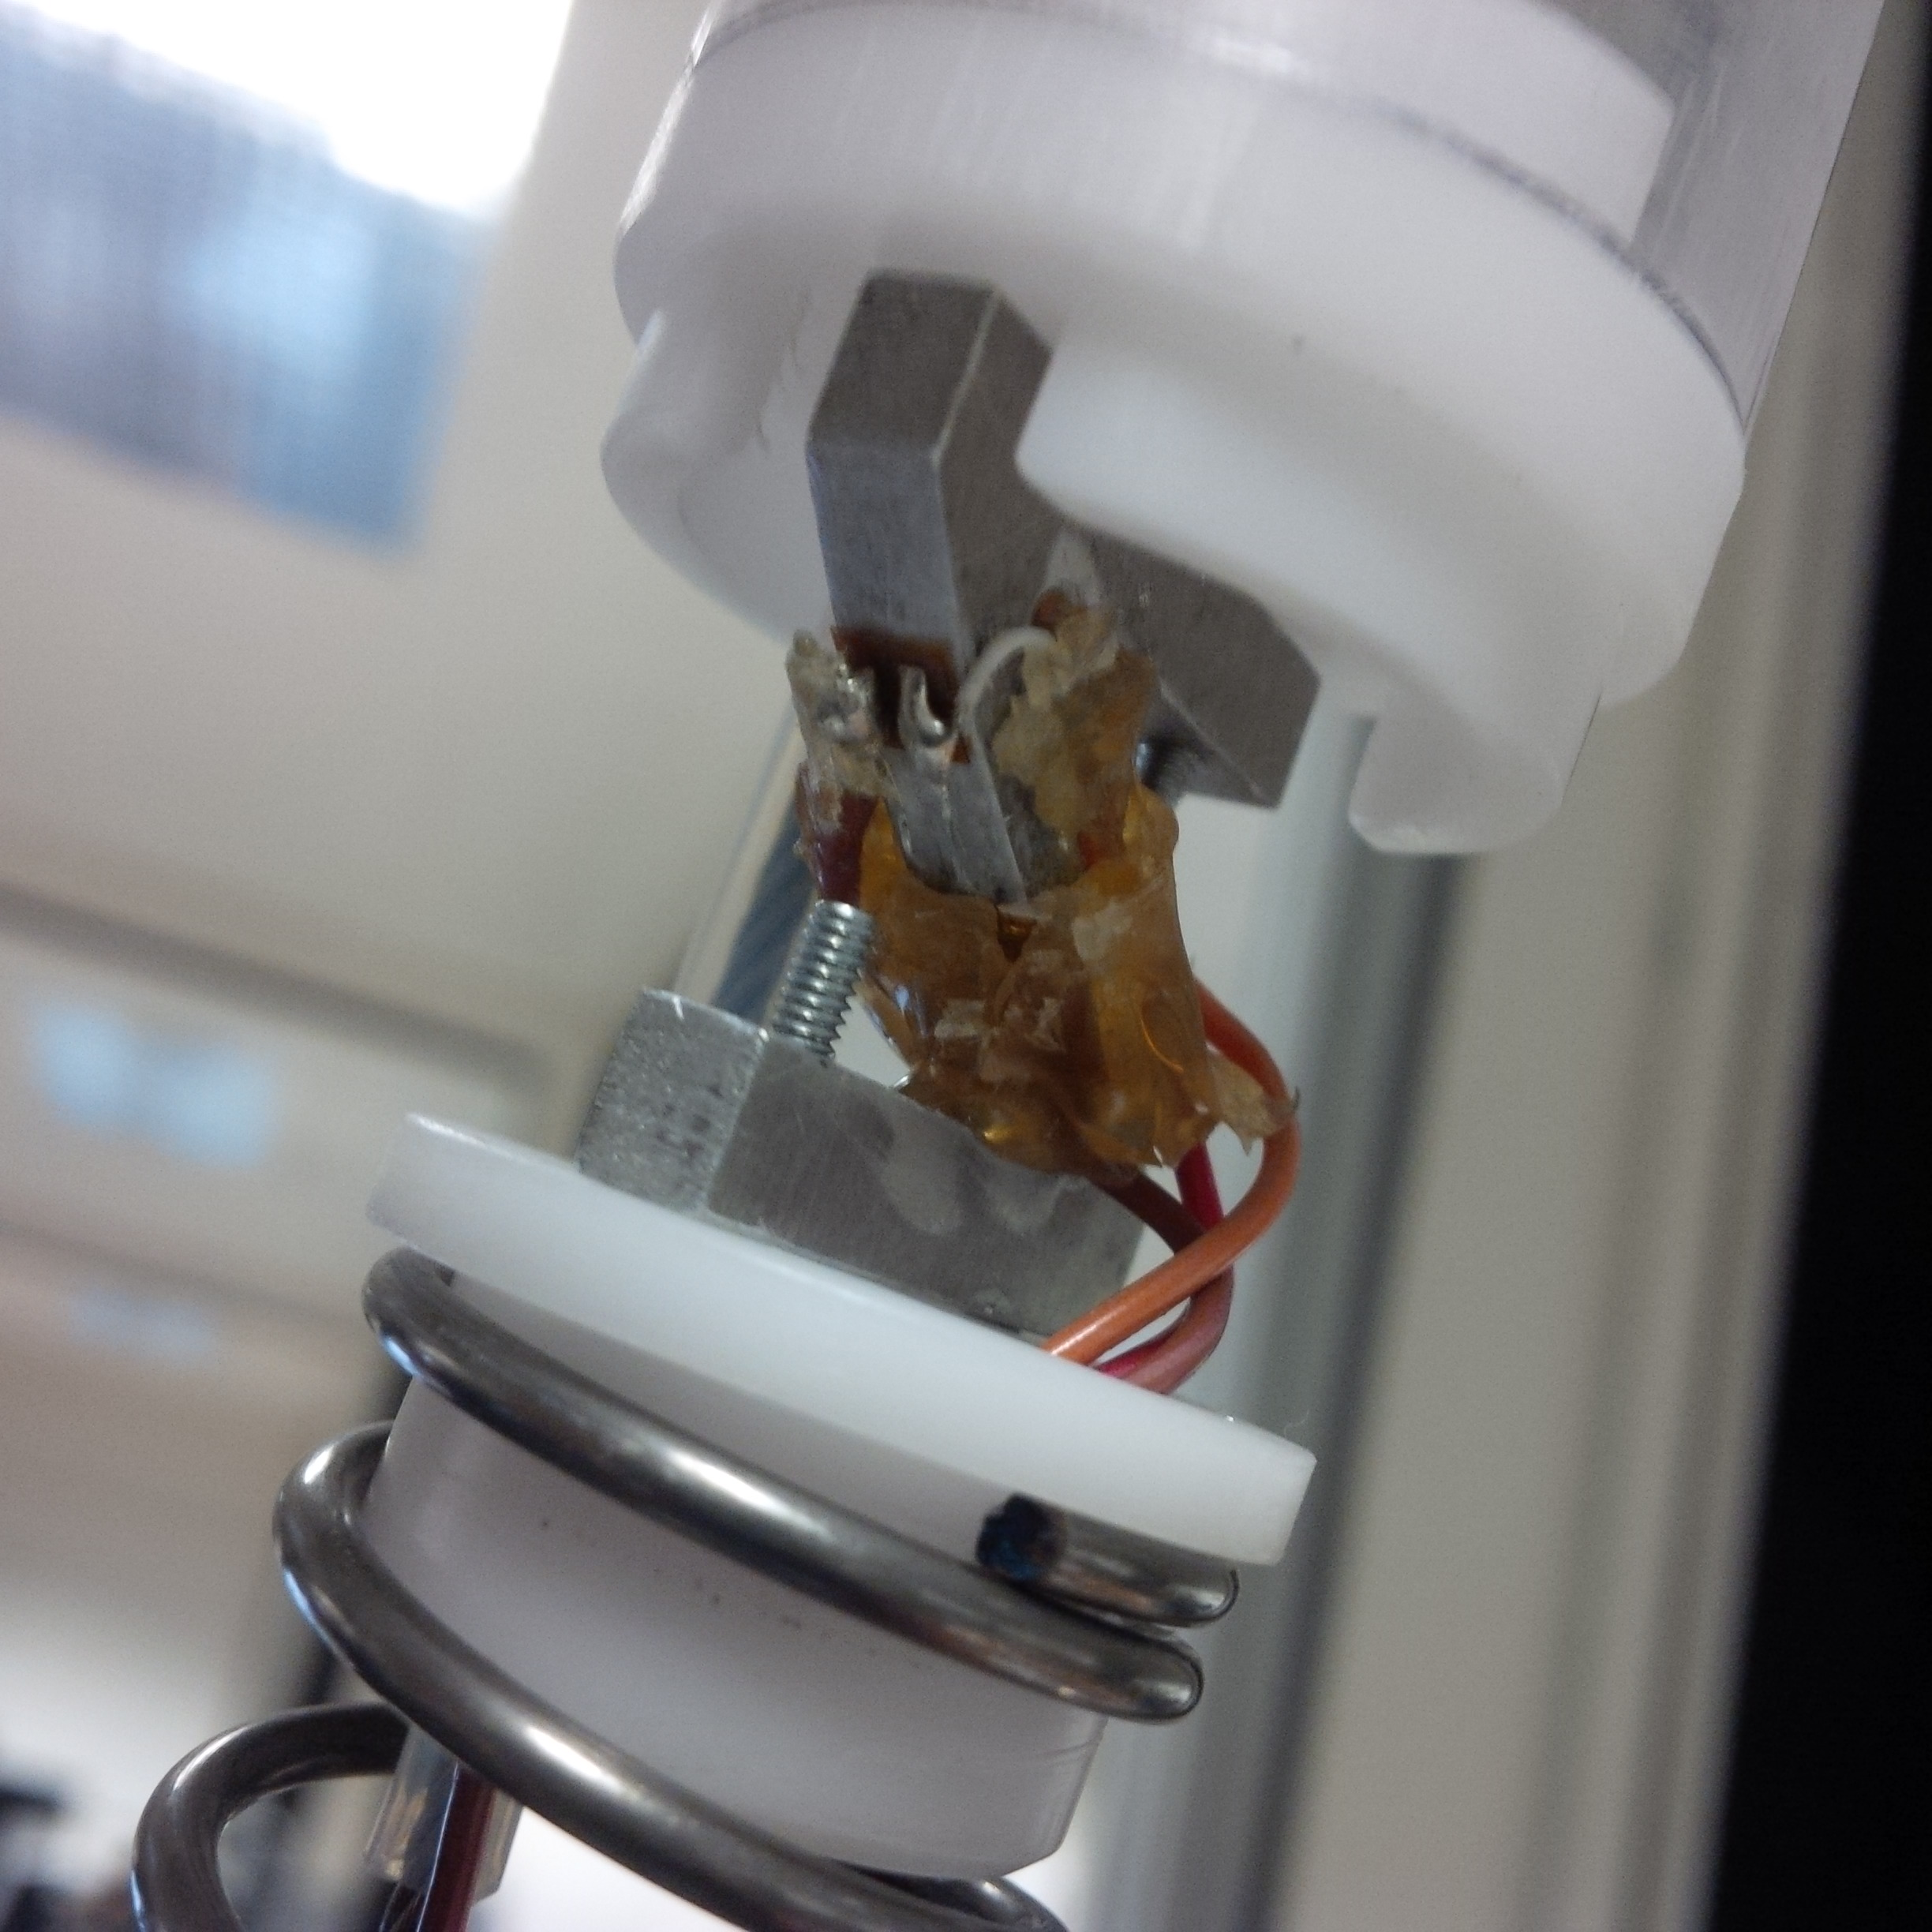
\includegraphics[width=.5\columnwidth]{img/SUPERball_compressive_gauge.jpg}
      \caption{Prototype of the axial compressive force sensor inside one of SUPERball's rod's spring assemblies. Note the thin cross-section that allows for cables (not shown here) to pass by vertically on each side of the Z-shape.}
      \label{fig:compressive_strain_gauge}
      \vspace{-0.2cm}
\end{figure}


The most recent prototype of these compressive sensors is shown in Figure \ref{fig:compressive_strain_gauge}.
Like other designs that were considered, it has a purely planar geometry so as to be manufactured by a water-jet machine out of sheet metal.
This design was chosen for a combination of effective response during testing and comparison of designs, as well as ease of assembly - the two strain gauges that are attached to each side of the middle deforming bar of the ``Z'' can be easily attached, as compared to e.g. circular designs.
These strain gauges are connected in a simple half-bridge circuit and connected to an ADC on one of SUPERball's circuitboards.

\begin{figure}[thpb]
      \centering
      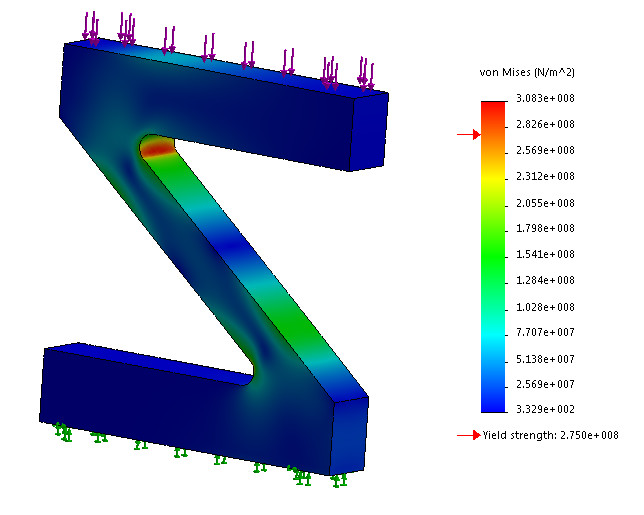
\includegraphics[width=.5\columnwidth]{img/Symmetric_Z_FEA.jpg}
      \caption{Predicted stress in the compressive force sensor using Solidworks FEA. Note that this plot shows meshing issues around the high-stress section.}
      \label{fig:compressive_strain_gauge_fea}
      \vspace{-0.2cm}
\end{figure}

Figure \ref{fig:compressive_strain_gauge_fea} shows a very simple axial compression FEA in Solidworks for this part.
Multiple iterations of FEA were used to design the dimensions of the Z-shape such that the gauge should not plastically deform (thus losing calibration) or otherwise fail under the maximum expected loading of the cables.
However, note that the final design in Figure \ref{fig:compressive_strain_gauge_fea} does show stress above yield - this was a consequence of Solidworks FEA's simplicity in meshing the bend in the Z, as shown by the sharp cutoff in the red high-stress area.
Each run of this simulation showed stress above yielding at a variety of applied forces, which implied the need for more advanced FEA procedures.
Due to time constraints, this was not pursued.

\subsection{Motor Mount Torque Sensor}

The second custom sensor on SUPERball is the torque sensor, which also functions as the motor mount.
Though designing a crucial piece of the actuator structure to intentially deflect risks significant issues with structural rigidity and stability, benefits for prototyping outweighed the risks.
Specifically, there was a need to implement low-level closed loop control directly on a single rod - closing a loop over a wireless radio would introduce too many issues with timing and control stability (and would complicate debugging during prototyping.)
Since only having the cable compression sensors would require that state estimation occurred over wireless (SUPERball's 6 rods are not electrically connected), options were considered to sense outgoing cable force on the same rod as the actuator.
As opposed to an additional part, this motor mount sensor allows direct measurement of the torque applied to the motor, and thus the force in the cable that is controlled by that motor.

\begin{figure}[thpb]
      \centering
      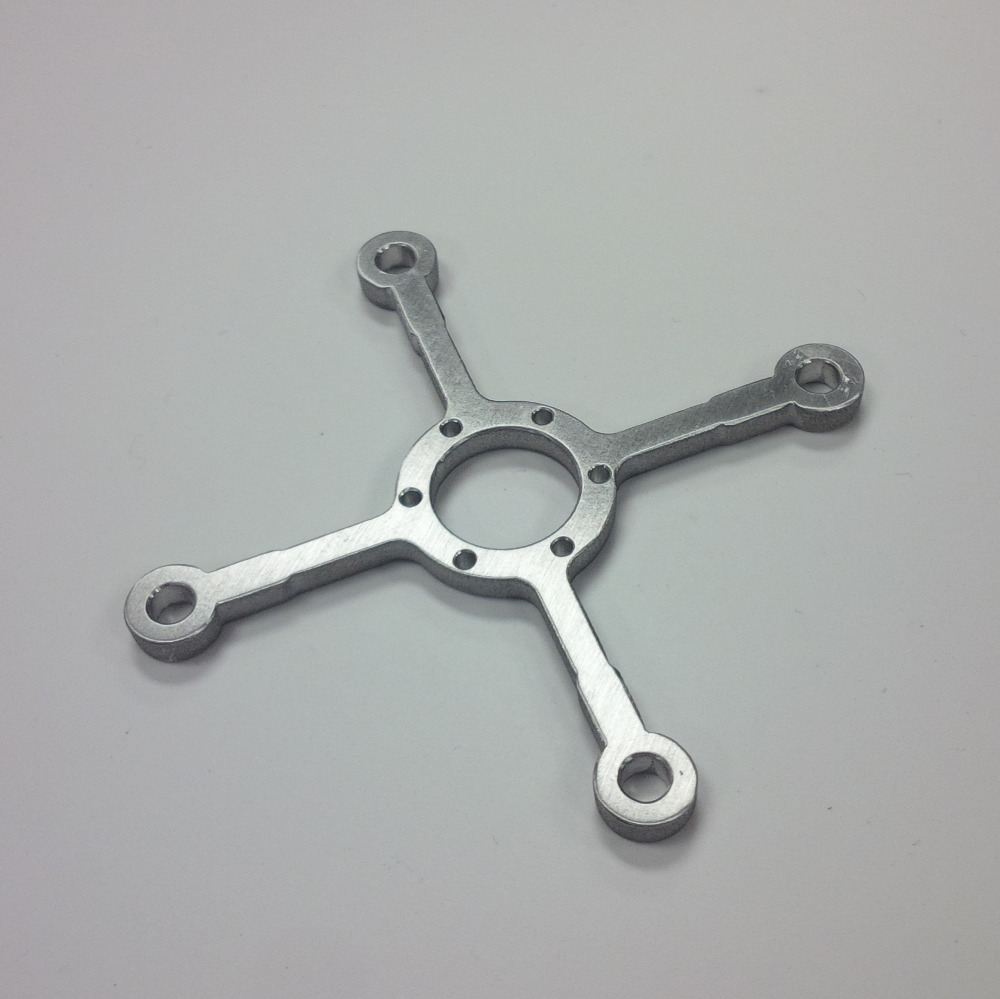
\includegraphics[width=.5\columnwidth]{img/motor_mount_torque_sensor.jpg}
      \caption{The bare metal cutout of the motor mount torque sensor structure. The center bolt pattern is for the motor attachment, and the four holes of the square outside pattern are for the supporting bolts of the actuator assembly onto which the motor mount slides.}
      \label{fig:motor_mount_torque_sensor}
      \vspace{-0.2cm}
\end{figure}

\begin{figure}[thpb]
      \centering
      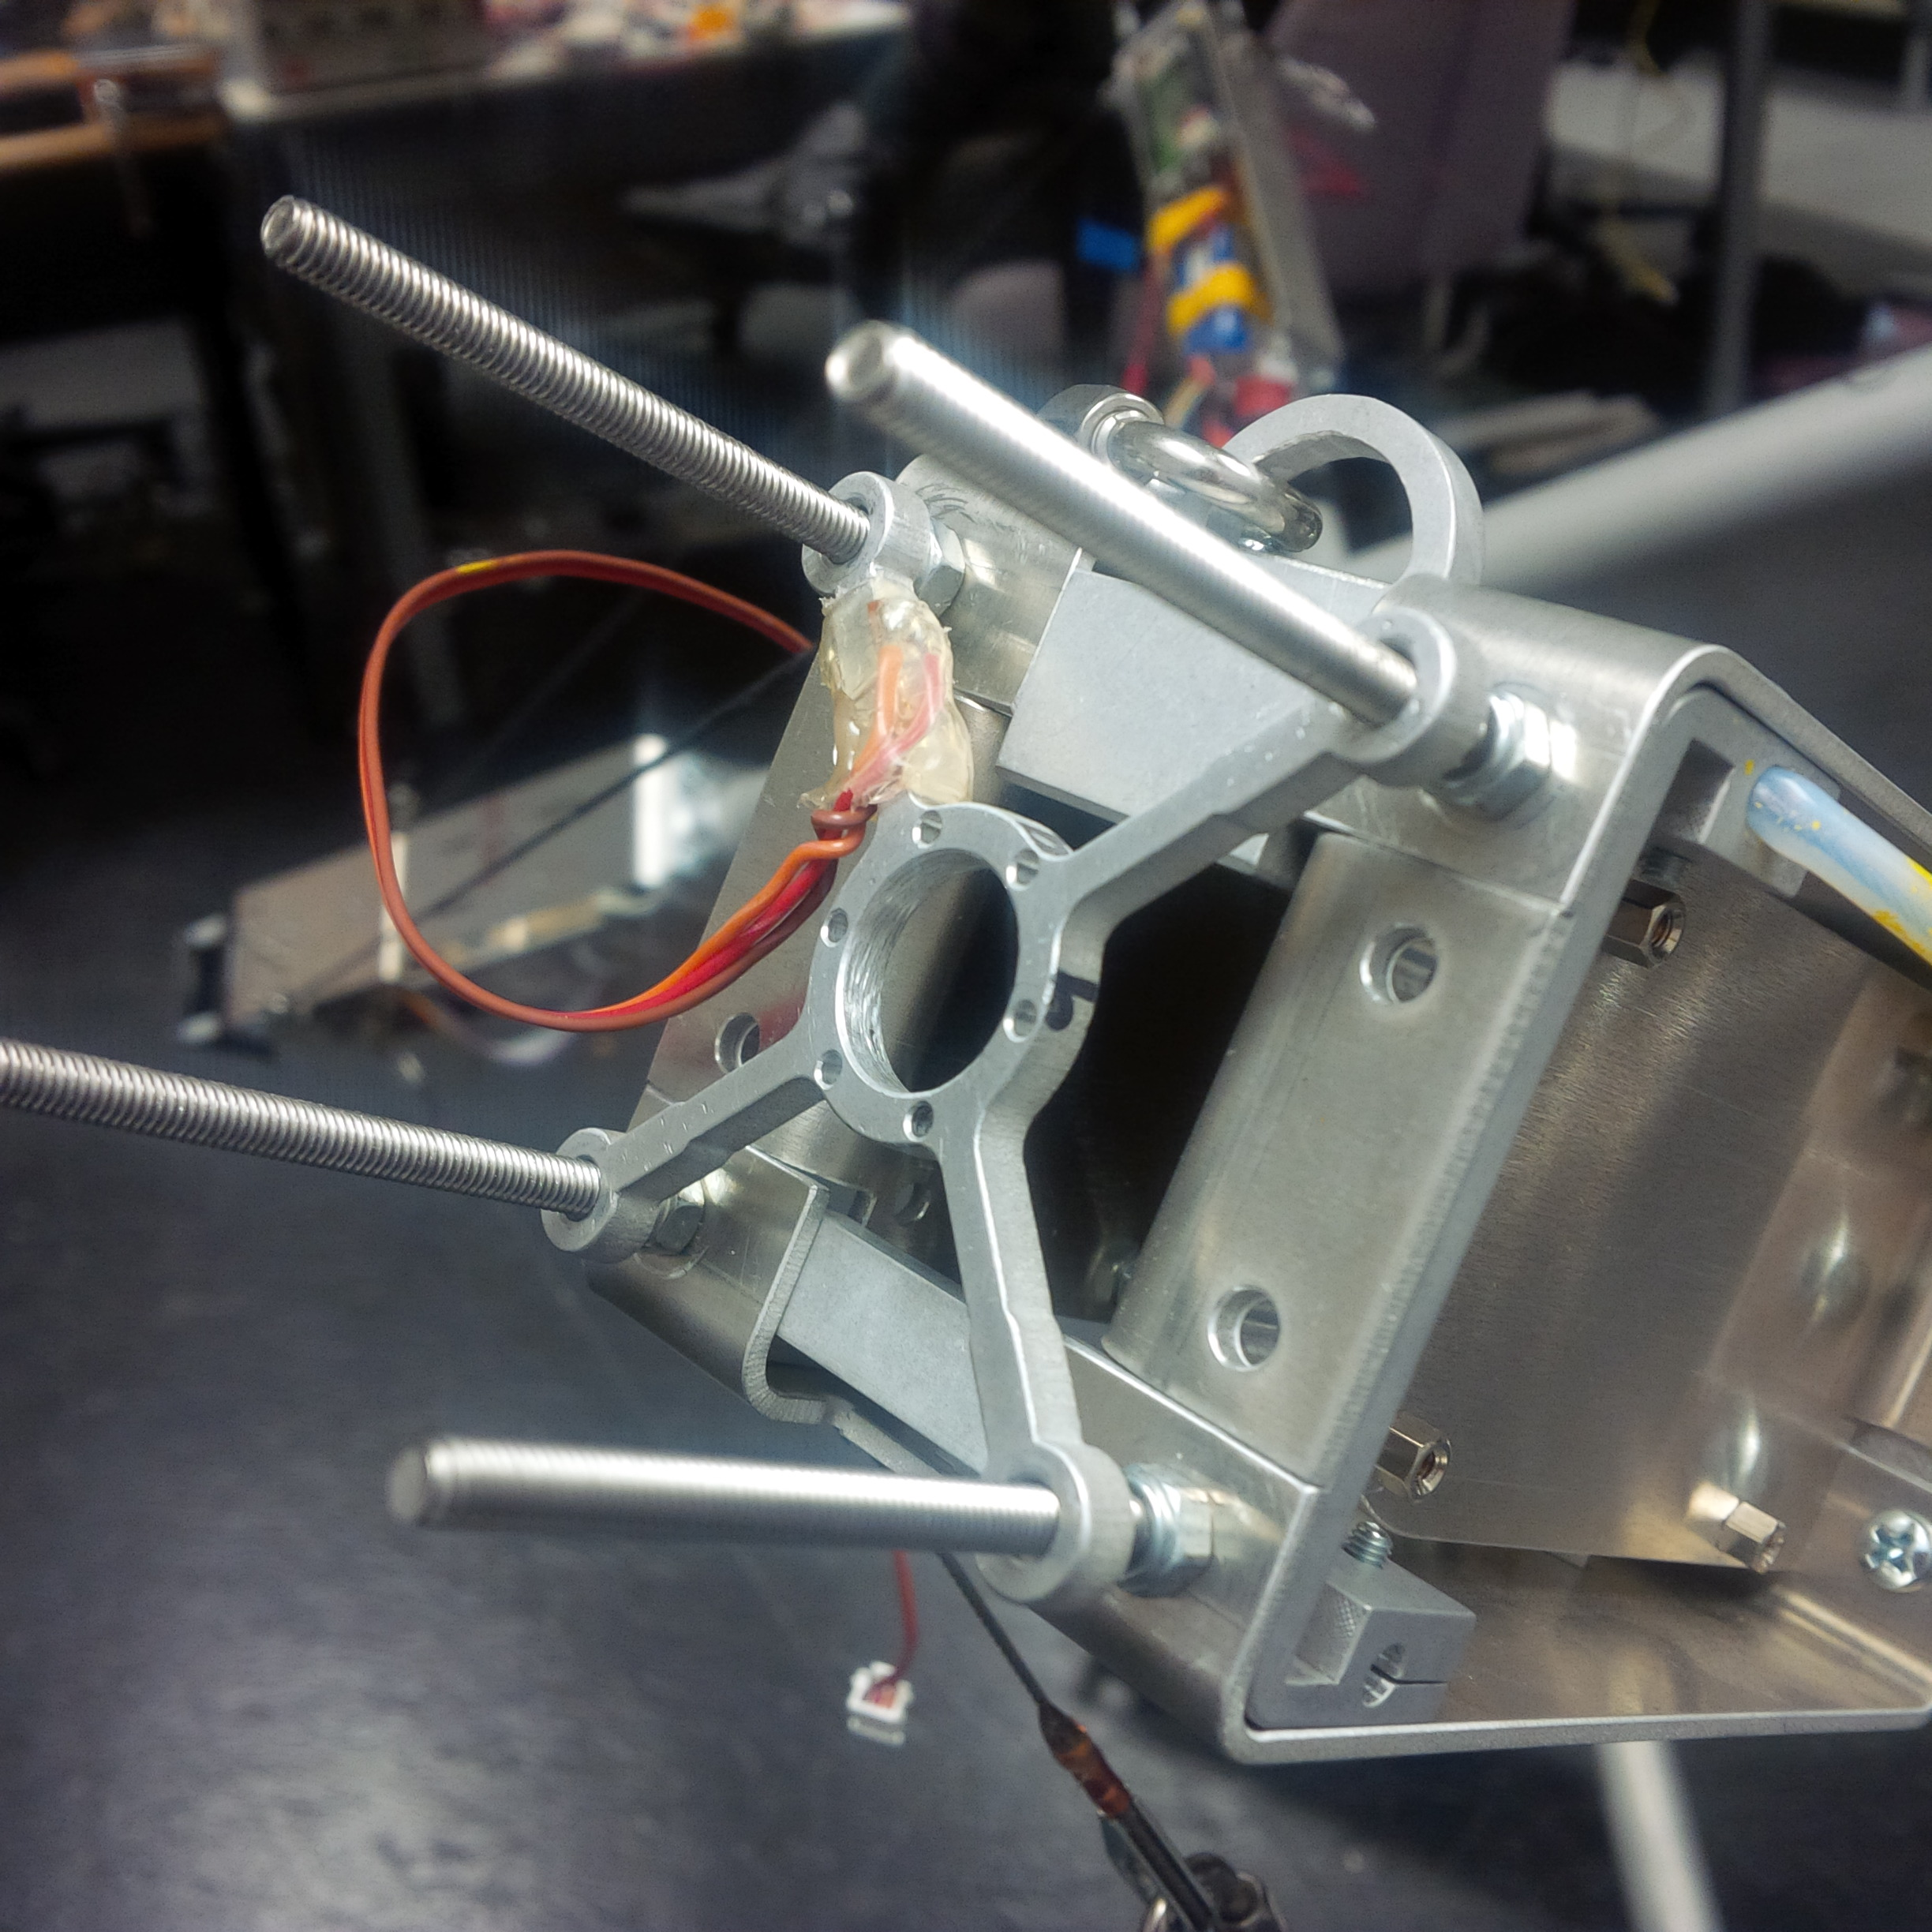
\includegraphics[width=.5\columnwidth]{img/sensor_onrod.jpg}
      \caption{A motor mount torque sensor fully assembled (with strain gauges) on one of SUPERball's rods. A motor would attach to the center of the sensor and fit between the two inner sheet metal side brackets.}
      \label{fig:motor_mount_torque_sensor_assembled}
      \vspace{-0.2cm}
\end{figure}

Figure \ref{fig:motor_mount_torque_sensor} shows one of these cross-shaped sensors without its strain gauges, freshly manufactured with a water-jet machine.
Figure \ref{fig:motor_mount_torque_sensor_assembled} shows a sensor that's been assembled, with the strain gauges attached, and which has been placed on the retaining bolts for the actuation assembly - though it does not have the motor attached.
The arms of the mount bend as the motor torques against it, and the half-bridge strain gauges are attached on opposite sides of one single arm. 
The motor is attached to the sensor/mount with six mounting bolts at the end of its gearbox.

This sensor's dimensions were also designed using Solidworks FEA to get appropriate dimensions of the cross-arms which deform.
However, since that was not my work, it is not included here.


%%%%%%%%%%%%%%%%%%%%%%%%%%%%%%%%%%%%%%%%%%%%%%%%%%%%%
% Testing - hardware, sensors
%%%%%%%%%%%%%%%%%%%%%%%%%%%%%%%%%%%%%%%%%%%%%%%%%%%%%

\chapter{Testing and Analysis}

\section{Structural System Testing and Analysis}\label{sec:hardware_testing}

Different types of tests were performed on each of these designs of the end-cap, in accordance with the component's importance in relation to the overall design goals for SUPERball.
In-depth testing was performed on subsystems whose failure modes were most severe, such as the structural subsystem.
However, even if not discussed explicitly below, a minimum of qualitative tests were performed for each part, to confirm a basic level of functionality.
Future work will include more thorough testing and calibration for all components.

\subsection{Analytical Safety Factor Predictions}

The failure modes of the structural load-bearing elements in SUPERball are most severe, and were thus analyzed with a variety of techniques.
First, analytical calculations were performed for failure modes of the structure, including the aluminum strut tube and sheet metal components.
These calculations were performed in the initial design phase for components with simpler geometries; see below for numerical tests of complex parts.

For the strut tube, two basic calculations included tests for failure in axial loading as well as buckling.
The force applied to the strut tube was calculated by assuming all eight cables attached to one rod applied the max load of 100N (from Table \ref{eng_requirements}), in line with the tube, for $F_a = 800N$.
At the inner/outer diameter cited above for this design, axial stress is then

\[
\sigma_a = \frac{F_a}{A} = \frac{800}{ \frac{\pi}{4} (r_o^2 - r_i^2) } = \frac{800}{ \frac{\pi}{4} ((0.00331)^2 - (0.00349)^2)} = 8.4 \ MPa
\]

This gives an axial compression failure safety factor of 32, using a yield strength of $\sigma_f$ = 269 MPa for the 2024-T3 aluminum alloy from which this tube is made~\cite{Aluminum2024_2014}. 
Similarly, using Euler's buckling approximation and a modulus of elasticity of $E =$ 73 GPa,

\[
F_{buckling} = \frac{\pi^2 E I}{(K L)^2} = \frac{\pi^2 (73 * 10^9) (\frac{\pi}{64} (0.00349^4 - 0.00331^4) )}{ (2) (1)} = 2480 \ N
\]

This gives a buckling failure safety factor of $2481 / 800 = 3.1$, which although small, is acceptable for this prototype.
Additionally, a 3D stress state was calculated, assuming this axial load as well as hoop and shear stresses from a torsional load of the same magnitude.
This last assumption was justified in the case of an incorrect tube placement: if the tube did not contact the face of the shaft collar, the entire $800N$ load would be transmitted through shear on the contact face.
Assuming a coefficient of static friction of $\mu = 0.95$ for aluminum against aluminum~\cite{AluminumFriction_2014}, and a contact length of 10mm, the tube pressure, hoop stress, and shear stress were calculated to be

\[
P_r = \frac{F_{pressure}}{A_{face}} = \frac{ 800/ \mu }{2 \pi r h} = \frac{ 800/ 0.95 }{2 \pi (0.0175) (0.01)} = 766 \ kPa
\]

\[
\sigma_h = \frac{P_r r}{t} = \frac{(766 * 10^3)(0.01657)}{8.89*10^-4} = 14.3 MPa
\]

\[
\tau_{yz} = \frac{F_{shear}}{A_{face}} = \frac{ 800 }{2 \pi r h} = \frac{ 800}{2 \pi (0.0175) (0.01)} = 727 \ kPa
\]

Note that in the above, the internal pressure on the thin-walled tube comes entirely from the clamping action of the shaft collar resisting the axial load.
The von Mises stress from this calculation can then be compared to the yield stress of 2024-T3 aluminum. In SI units of MPa,

\[
\boldsymbol{\sigma} = \left[ \begin{array}{ccc}
    \sigma_h & \tau_{xz} & \tau_{xy} \\
    \tau_{xz} & \sigma_a & \tau_{yz} \\
    \tau_{xy} & \tau_{yz} & \sigma_r
\end{array} \right]
=
\left[ \begin{array}{ccc}
    14.3 & 0 & 0 \\
    0 & 8.4 & (0.727) \\
    0 & (0.727) & (0.766)
\end{array} \right],
\quad
\sigma_{vm} = 11.82 \ MPa
\]

This is larger than the original axial stress estimate, taking the compression failure safety factor down to $269/11.82 = 22$.
From all this analysis, it is clear that the failure mode of the strut tube would be buckling, which currently has the small but acceptable safety factor of 3.

%\textcolor{red}{Insert analysis of the sheet metal brackets, from Dizhou's thesis.}
For the sheet metal brackets, a similar buckling analysis was performed. 
Here, similar properties of aluminum were used, with $\nu = 0.33$~\cite{Aluminum2024_2014}.
Approximating each bent bracket as simply-supported, and assuming the bending process has not weakened the material significantly, the edge most likely to buckle is one long side of the battery compartment.
This section that is 0.11m long with a cross-sectional area of 2mm by 60mm has a critical buckling force \cite{rees2009optimal} of:

\[
P_{cr} = \frac{\pi^2 E I}{(1-\nu^2)a^2} = \frac{ \pi^2 (69*10^9)(\frac{1}{12} (0.06)(0.002)^3)}{(1-(0.33)^2)(0.11)^2} = 2530 N
\]

Compared against a maximum worst-case load of $800N$ from above, this bracket has a safety factor against buckling of $2530/800 = 3.1$, which like the tube, is small but acceptable for a prototype. \\

\subsection{Numerical Safety Factor Predictions}
%Numerical: FEA, ANSYS for the endcap shaft collar.
%Want to include Solidworks FEA for: Battery Compartment, Motor mount torque sensor, Brake Cable Guide, Spool Cap Bottom, ...?

% For each FEA test, need to describe: 
% 1) the material properties used
% 2) the mesh used, and what type of element
% 3) the constraints applied,
% 4) the forces and loads applied,
% 5) the results: the max von Mises stress.

\begin{figure}[thbt]
  \begin{center}
    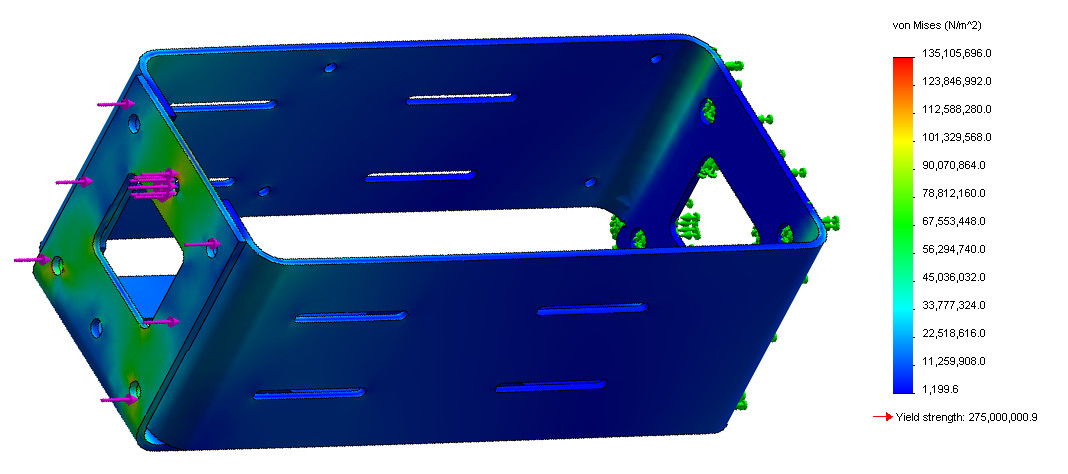
\includegraphics[width=0.75\textwidth]{./img/battery_compartment_compression_test_edited.jpg}
    \caption{FEA Test of the battery compartment, with 800N load and bonded contact surfaces.}
    \label{battery_compartment_FEA}
  \end{center}
\end{figure}

\begin{wrapfigure}{R}{0.4\columnwidth}
   \centering
   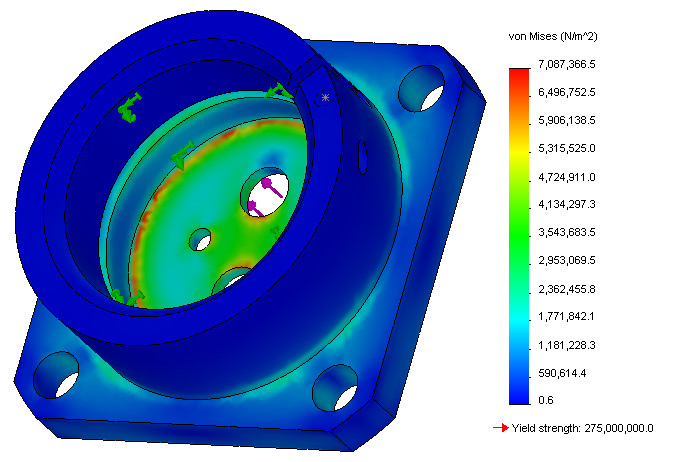
\includegraphics[width=0.4\columnwidth]{img/endcap_shaft_collar_compression_test_800N_edited.jpg} 
   \caption{FEA test of the end-cap shaft collar.}
   \label{endcap_shaft_collar_FEA}
%%   \vspace{-0.5cm}
\end{wrapfigure}

In addition to an analytical estimation of the factor of safety for parts with simpler geometries, finite element analysis tests were conducted for the other structural components.
Specificallly, the end-cap shaft collar, battery compartment, and bottom spool cap were tested within Solidworks Simulation 2012.
Each test was done as a compression test with the same worst-case load as estimated above of 800N.

\begin{wrapfigure}{r}{0.4\columnwidth}
   \centering
   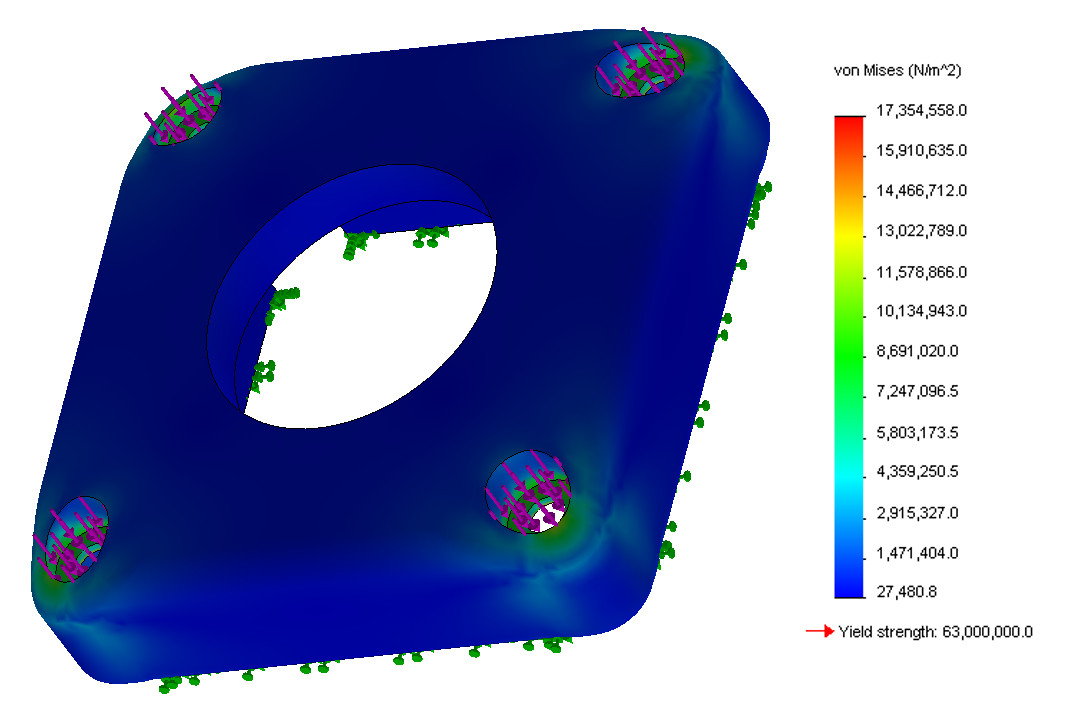
\includegraphics[width=0.4\columnwidth]{img/bottom_spool_cap_compression_test_edited.jpg} 
   \caption{FEA test of the bottom spool cap part.}
   \label{bottom_spool_cap_100N}
%%   \vspace{-0.5cm}
\end{wrapfigure}

The end-cap shaft collar test, shown in Figure \ref{endcap_shaft_collar_FEA}, used the default material properties within Solidworks for 6061-T6 aluminum.
The default mesh type was used, with a global element size of 1.75mm.
The inner cylindrical face, where the collar clamps the strut tube, was constrained in all six degrees of freedom (fully built-in.)
Then, a force of 800N was applied to the top face, where the battery compartment would attach.
As expected, since this part was still relatively thick-walled, this test showed a maximum von Mises stress of only 7 MPa, so this part had an estimated safety factor of 38 against the yield strength of 269 MPa.
This indicated that the shaft collar piece was not a source of concern for failure.

The static compression test of the battery compartment, shown in Figure \ref{battery_compartment_FEA}, also used the default material properties within Solidworks for 6061-T6 aluminum. 
The default mesh type and size were also used.
The bottom face, which contacts the end-cap shaft collar, was constrained in all six degrees of freedom.
The topmost bent face, which bolts to the structural brackets surrounding the motor, had an applied normal load of 800N.

Additionally, the Solidworks ``Component Contact: Bonded'' of two faces was applied between the three bent pieces of sheet metal at the top of the compartment that are compressed together when bolted.
The test in Figure \ref{battery_compartment_FEA} shows a maximum von Mises stress of 135 MPa, leading to a safety factor of almost 2.

%\begin{wrapfigure}{r}{0.4\columnwidth}
%   \centering
%   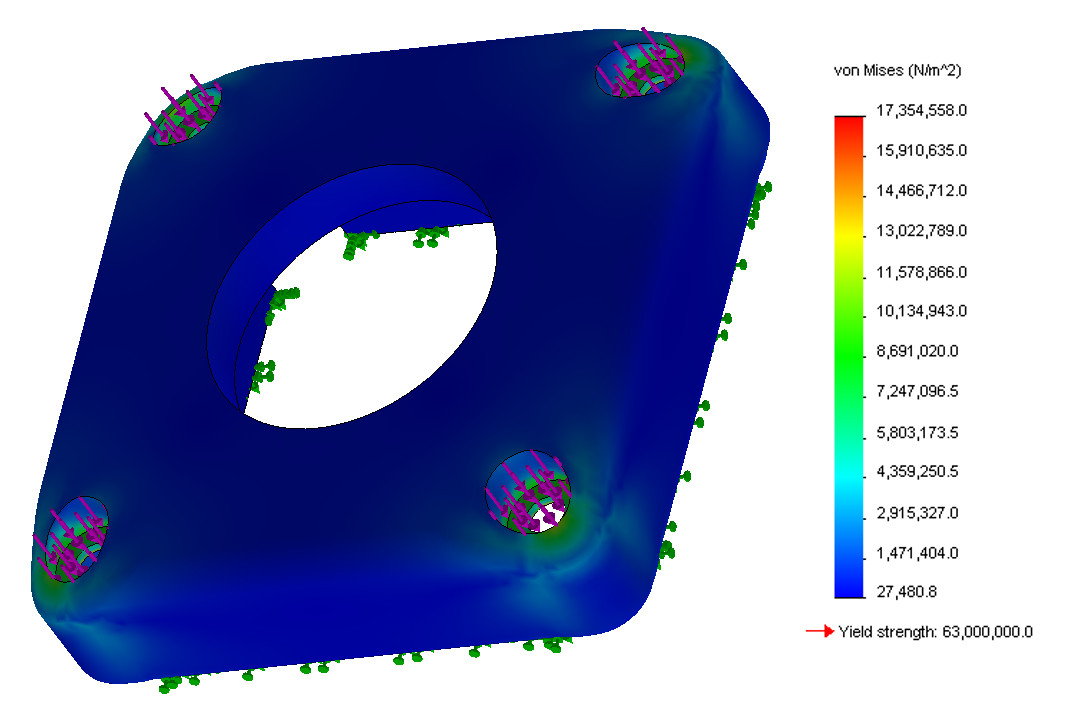
\includegraphics[width=0.4\columnwidth]{img/bottom_spool_cap_compression_test_edited.jpg} 
%   \caption{FEA test of the bottom spool cap part.}
%   \label{bottom_spool_cap_100N}
%%   \vspace{-0.5cm}
%\end{wrapfigure}

This compares decently well with the simplistic stress calculation above, but does indicate that the initial simplistic calculations do not account for the bends in the sheet metal.
Note that a bending test in FEA is not included in these results due to failures of the simulation to find a solution.

Two static compression tests of the bottom spool cap were also conducted, using the default material properties within Solidworks Simulation 2012 for Delrin acetyl resin, the raw material from which the part is made.
The faces which contact the supporting sheet metal brackets were constrained in all six degrees of freedom. %maybe show which surfaces these are?
As before, the default mesh type and size were also used.
Among the many forces this cap could experience, the compressive force on its inner flanges from the nylon spacers is expected to be most significant.
As discussed above, these flanges transmit the entire load of impact of the rod end, as well as any loads from the radial bearing of the motor spindle.
Two different tests were performed with loads of 100N and 800N.
The former, shown in Figure \ref{bottom_spool_cap_100N}, was justified as a lower-end estimate of the force a rod would experience from its one actuated cable.
For this smaller load, the maximum von Mises stress was 17 MPa, for a safety factor of 4.2 using the value of 72 MPa as the yield strength of Delrin~\cite{Delrin2014}.
However, the test with the larger load of 800N (worst case) showed a maximum von Mises stress of 133 MPa, which was a factor of 8 larger than the other test as expected.
This larger value would cause failure in the part, and thus helped identify this as a potential failure mode and candidate for future redesign. \\

\begin{figure}[hbt]
  \begin{center}
    \begin{subfigure}[b]{0.45\textwidth}
      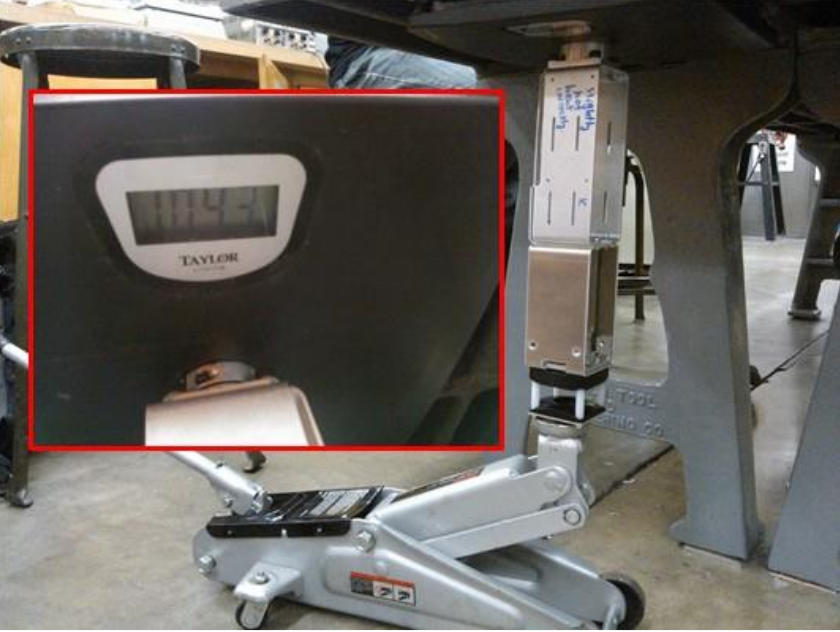
\includegraphics[width=1\textwidth]{./img/compression_test.jpg}
      \caption{Compression test setup for end-cap prototype.}
      \label{endcap_compression_test_experimental}
    \end{subfigure}
    \begin{subfigure}[b]{0.45\textwidth}
      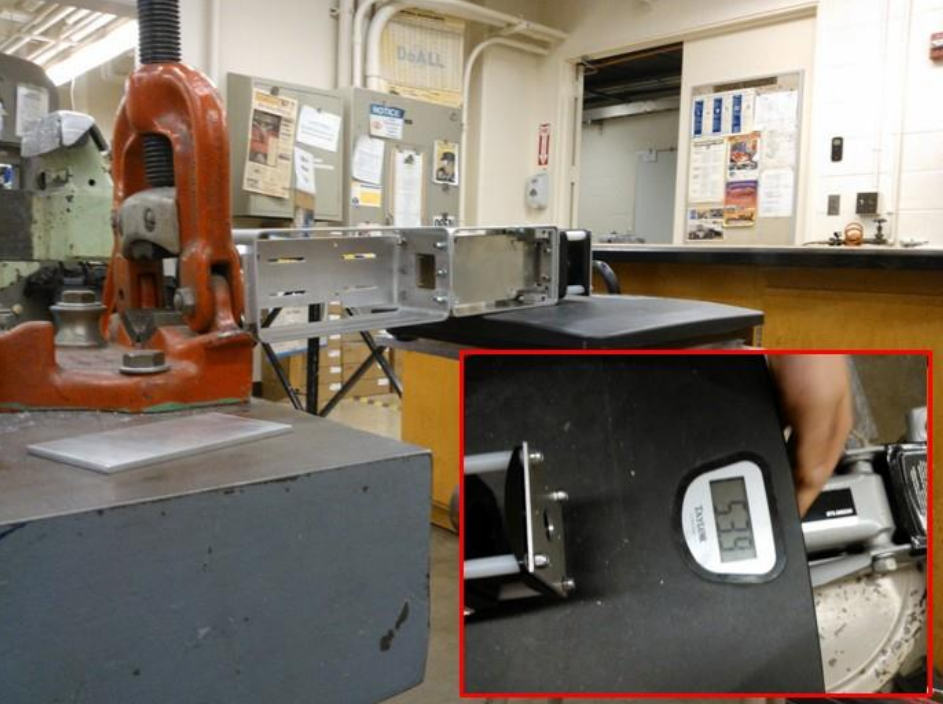
\includegraphics[width=1\textwidth]{./img/bending_test.jpg}
      \caption{Bending test setup for end-cap prototype.}
      \label{endcap_bending_test_experimental}
    \end{subfigure}
  \end{center}
%  \vspace{-0.5cm}
\end{figure}

%\vspace{-0.5cm}

\subsection{Experimental Testing}

\begin{wrapfigure}{R}{0.40\columnwidth}
   \vspace{-0.5cm}
   \centering
   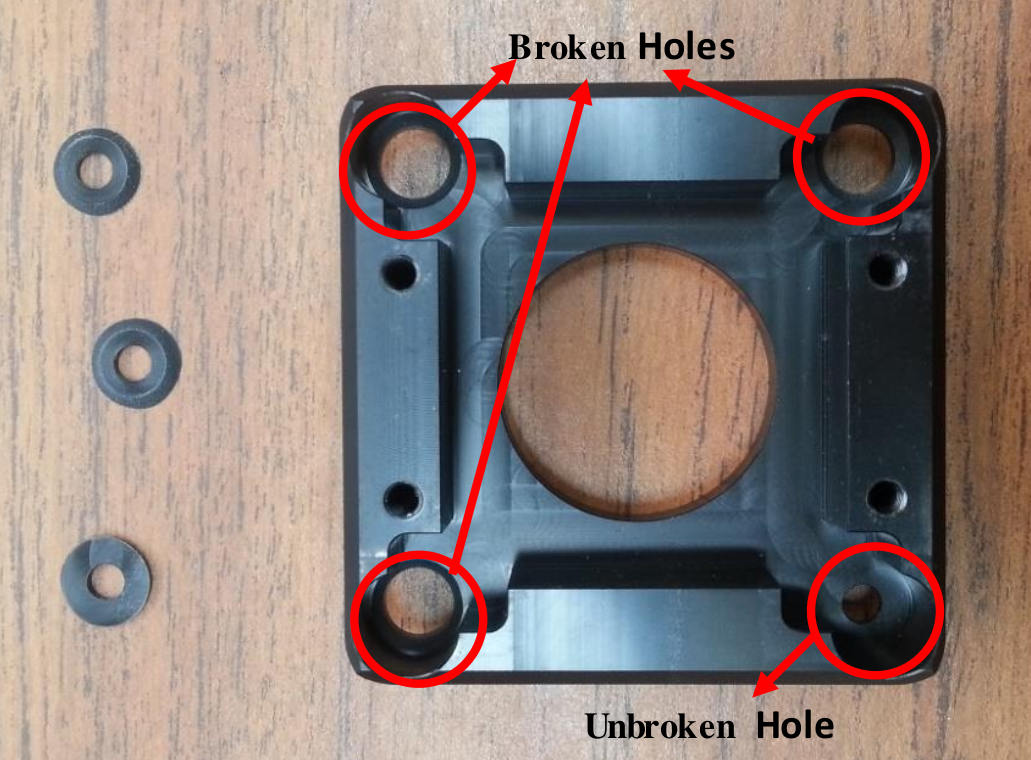
\includegraphics[width=0.40\columnwidth]{img/bottom_spool_cap_failure.jpg} 
   \caption{Results from compression test. Flanges on bottom spool cap have sheared, confirming the factor-of-safety predicted by the FEA results.}
   \label{broken_bottom_spool_cap}
   \vspace{-0.5cm}
\end{wrapfigure}

A final set of experimental tests were conducted with a full prototype of the end-cap assembly.
First, tests in compression and bending were performed, in order to validate various conclusions of the analytical and FEA tests.
Finally, a short drop test was performed that sought to mimic some of the conditions this robot might experience in the future when used as a planetary rover.
Note that none of the tests were performed until failure of the sheet metal, since practical considerations required re-use of these specific components.

An assembled end-cap, in its rig for the compression test, is shown in Figure \ref{endcap_compression_test_experimental}.
This low-fidelity test placed the end-cap, in series with a scale, between a hydraulic jack and a fixed support.
Increasing force from the jack up to approximately 1000N, just over the worst-case estimate of 800N.
For the sheet metal brackets and end-cap, no plastic deformation or failure was detected during this test, indicating that the assembly would survive such forces.
However, as shown in Figure \ref{broken_bottom_spool_cap}, the bottom spool cap flanges did indeed shear off as suggested by the FEA test.
Thus, a future redesign of these flanges would be required if such large forces were to be applied in practice.

Similarly, Figure \ref{endcap_bending_test_experimental} shows a test of a bending moment on the end-cap.
Although no such force is expected to be applied to the structure, and was not designed for, this test was performed as a precaution against unexpected situations during locomotion testing of this prototype.
The end-cap was horizontally clamped to a fixture, and then the scale was again placed in series with the hydraulic jack, which was used to apply a force of $54 N$ to the rod end section of the end-cap.
Again, no failure of any type was detected during tests, indicating that the assembly's robustness to unintentional collisions or loads.

Finally, a short drop test was performed using a fishing line as a guide for the end-cap and strut assembly to hit the ground at a specified angle.
% CHANGE ME
% Refer to table 1 for 800N metric.
The left of Figure \ref{endcap_drop_test_results} shows the test setup.
A piece of fishing line was attached to a fixture roughly 20 feet above a dirt and gravel bed, and then fixed into place in the ground at a net angle of roughly 60 degrees.
This height of about 20 feet corresponds to one-fifth the total energy with which a SUPERball would collide with the surface of Titan, Saturn's moon \cite{Vytas_IPPW_2013}.
Then, the end-cap assembly, attached to a strut tube, was placed on this fishing line and dropped.
The right image of Figure \ref{endcap_drop_test_results} shows the results of this drop test: the flanges in the bottom spool cap, previous identified as a potential location of failure, did indeed shear apart upon impact.
In this case, the nylon spacers forced the flanges apart from the cap body, and are lodged into the space below the cap.
Additionally, one long stainless steel M4 screw (inside the nylon spacer) deformed slightly.
This test identified areas of improvement for future revisions that would be hardened against larger drop tests: the sheet metal aluminum structure performed as expected, but the Delrin part and thin M4 bolt should be redesigned.

\begin{figure}[hbt]
  \begin{center}
    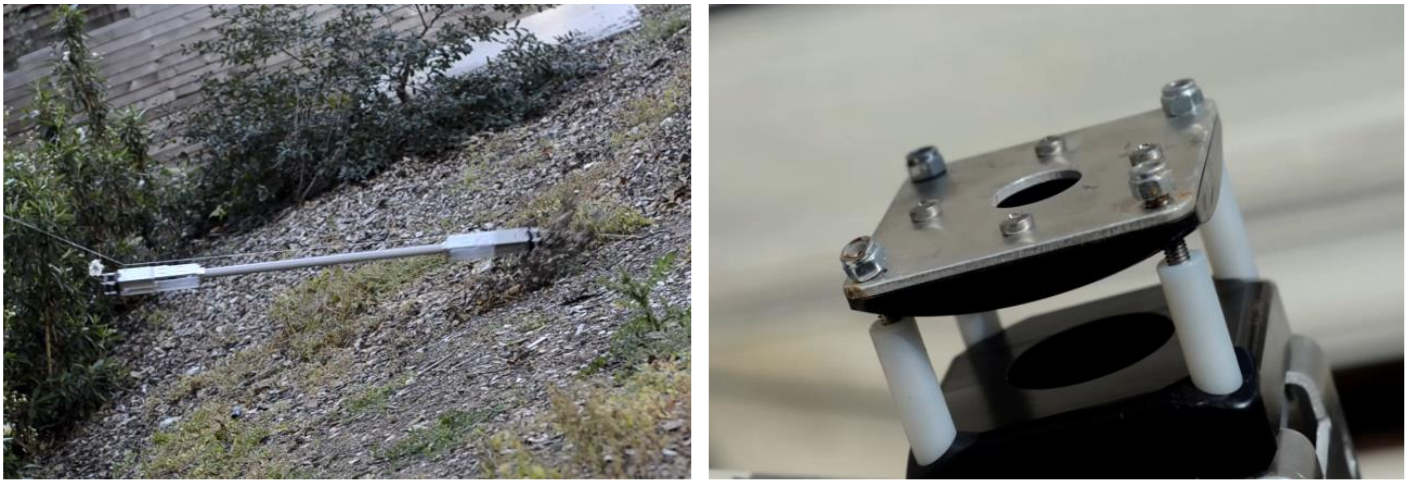
\includegraphics[width=0.95\textwidth]{./img/drop_test_results.jpg}
    \caption{Results of drop test. Left: End-cap and rod impact the ground. Right: Close-up of end-cap actuation area after impact, where the flanges on bottom spool cap have again sheared as the nylon spacers push through. Note that these forces are much greater than those expected under locomotion.}
    \label{endcap_drop_test_results}
  \end{center}
\end{figure}

All of these tests showed the basic validity of the structure used for SUPERball.
Although a more thorough confirmation of results would include tests until failure for metal parts, as well as a wider variety of tests, these were sufficient for the purposes of this prototype.
These structural tests show that this robot is unlikely to break during its locomotion tests, and that the operators are likely safe when performing such dynamic tests.


\section{Sensor Analysis}

Both of the 2 custom sensors on SUPERball were tested to different extents.
The following sections describe the analysis, debugging, and calibration of the two sensor types.

\subsection{Compression Sensor Analysis}

%We designed a compression sensor, since a preliminary review of COTS compo

Since the goal of this project was to show locomotion, work was concentrated on aspects of SUPERball that were necessary for basic control and estimation.
The low-level brushless motor feedback loop relied on the motor mount torque sensor, and thus the spring compression force sensor received less attention.
As of this writing, the compression sensors are not actively used on SUPERball, though redesigns are planned for the near future.

\begin{figure}[thpb]
      \centering
      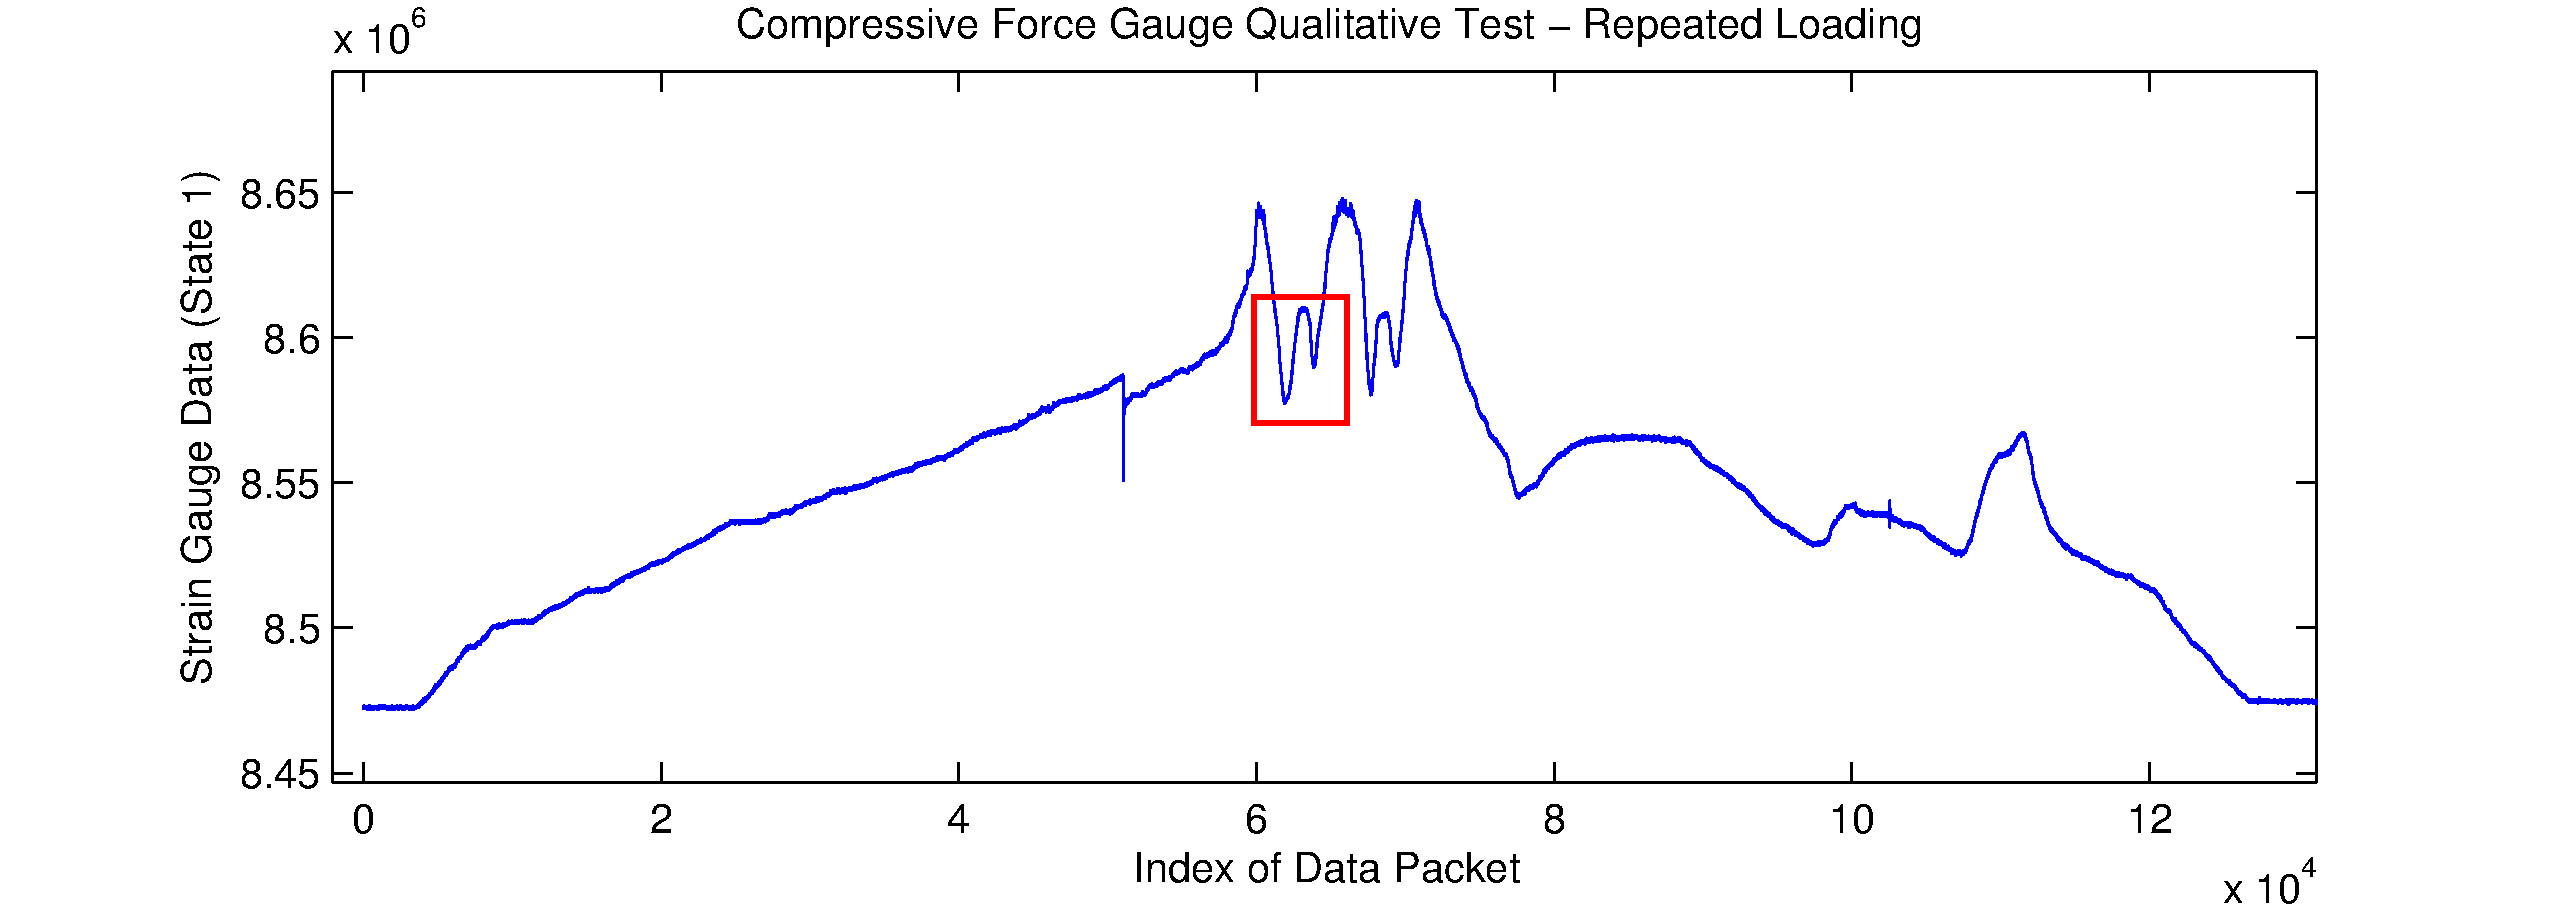
\includegraphics[width=0.9\columnwidth]{img/rodtest_slow.jpg}
      \caption{Data from a qualitative test of the compressive strain gauge inside a spring-cable assembly. Vertical axis is the raw output measurement from the 24-bit ADC, horizontal axis is sample number (e.g. time). Note that even though the cable was smoothly repeatedly loaded, the spring buckling causes undesired noise highlighted in the red box.}
      \label{fig:compression_sensor_data}
      \vspace{-0.2cm}
\end{figure}

Some qualitative testing was done with these sensors to show that they performed adequately, had the designers decided to manufacture the required 24 of them for the SUPERball prototype.
The data shown in Figure \ref{fig:compression_sensor_data} shows the measured response of the sensor when undergoing a simple qualitative test of pulling on a cable and thereby compressing the spring.
Meaningful responses are recorded for the duration of the test, from no-load until an individual compression spring was fully compressed.
However, this test revealed a significant issue with the spring design: since the outer diameter of these springs is less than the inner diameter of their enclosure tubes by about 5 mm, there is room for the compression springs to buckle.
This causes the dramatic noise during the repetitions of cyclic load of the cable, highlighted by the red box in Figure \ref{fig:compression_sensor_data}.
Additionally, such buckling can be seen in Figure \ref{fig:spring_buckling}, where the aliasing in the spring coils is due to such buckling.
Along with the emphasis on the other sensors for basic functionality, this buckling phenomenon influenced our decision to not pursue these designs before the first prototype.
For that first prototype, these sensors were just cut out from the sheet metal but not fully assembled with strain gauges.

\begin{figure}[thpb]
      \centering
      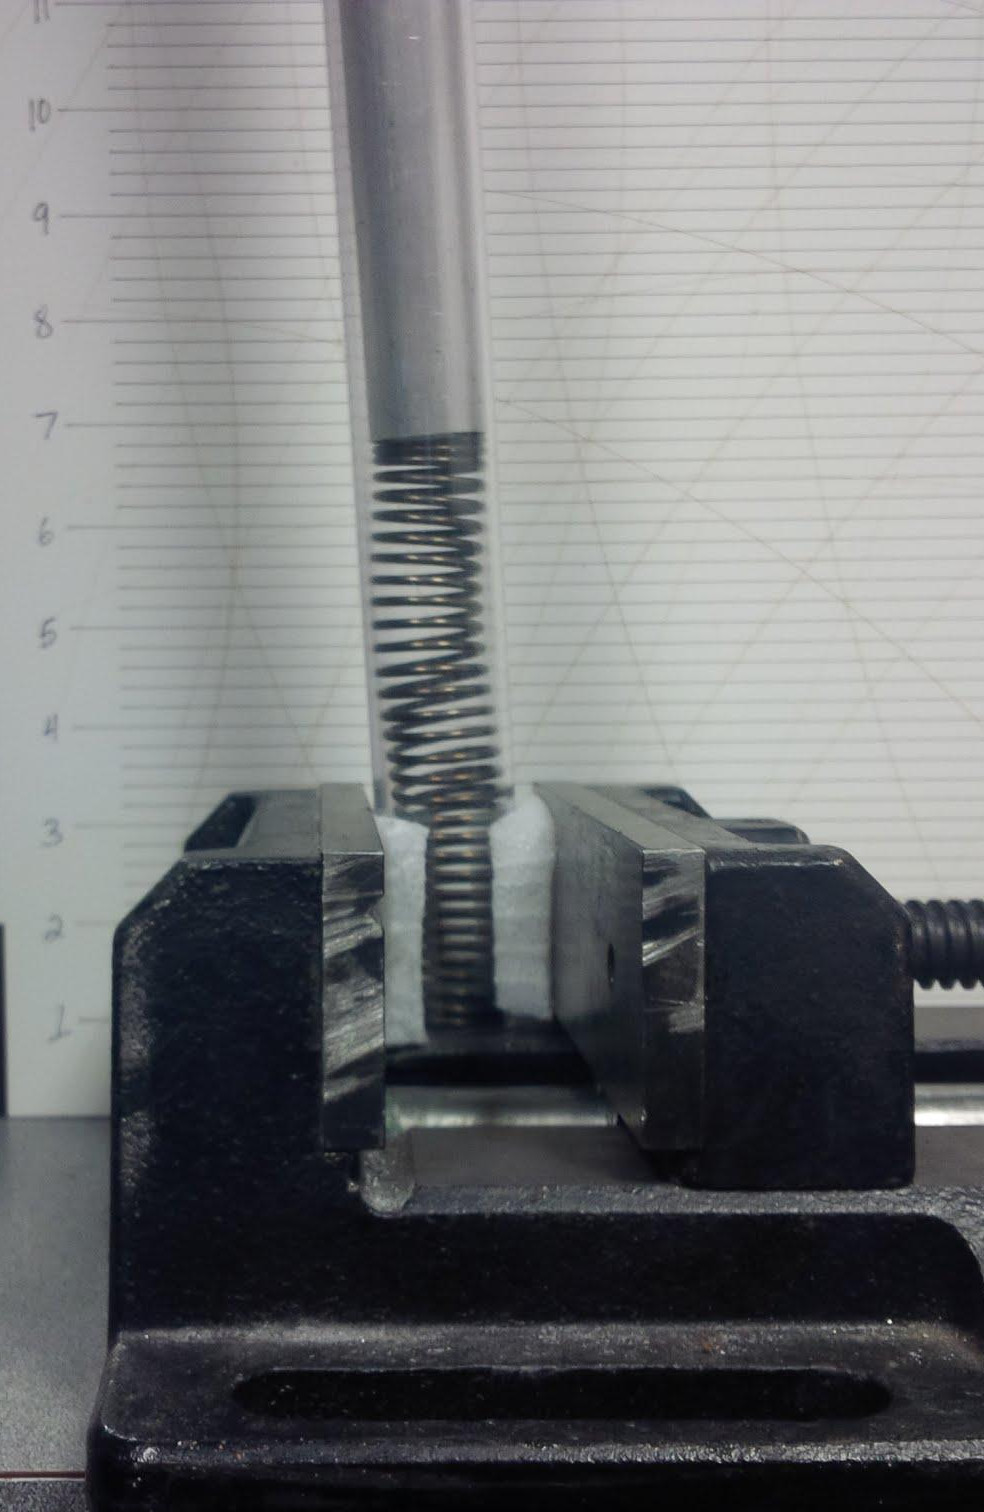
\includegraphics[width=.5\columnwidth]{img/spring_buckling_cropped.jpg}
      \caption{Test to confirm buckling phenomenon in SUPERball's spring tube assembly. Here, one of the springs is inserted into its tube, with the holder cap on the bottom, then clamped into place on a table. A force is then applied to the spring by using a long metal rod. Buckling is evident by the curving aliased coils in this image.}
      \label{fig:spring_buckling}
      \vspace{-0.2cm}
\end{figure}

Not captured by this data is the plastic deformation that some of these sensors experienced.
Many of these Z-shaped sensor prototypes became permanently bent after testing.
It is believed that this is partially a consequence of the internal compression spring buckling issue, however, this also implies that our team did not undertake thorough enough FEA analysis and that the results from Figure \ref{fig:compressive_strain_gauge_fea} are more accurate than was first thought.
Nonetheless, these sensors are scheduled for a redesign in upcoming SUPERball revisions to reduce plastic deformation.
Another examination of COTS parts will also be performed, so as to attempt to find a sensor which fits the required dimensions and also reduced the possibility of error from custom-made sensors.

\subsection{Torsional Sensor Calibration}

The motor mount torque sensor was qualitatively tested, and 12 of them were calibrated for use on SUPERball.
For calibration, hanging weights were used such that when hung off a given moment arm from a torsional sensor, they would enact a known torque.
Then, by using the radius of the spindle, these values can be converted into estimated force on a cable.
Recording the voltage across the sensor half-bridge for each of these data points allows for curve fitting for cable force.

I led two of our lab's fantastic undergraduates (Sarah Dobi and Roya Fallah Firoozi) in designing the following test rig, with four components.
The primary housing holds a radial bearing and the inner supporting shaft, which together model the motor and restrict measurements to the tangential degree of freedom (the bearing reduces out-of-plane motion.)
The sensor is then bolted onto the main housing, imitating the assembly onto the actuator bolts on a SUPERball endcap.
Figure \ref{fig:sensor_test_setup_exposed} shows this stage of assembly, with the sensor exposed.
Finally, an outer plate is attached that clamps onto the inner supporting shaft and whose bolts pass through the sensor's inner bolt pattern.
This allows the sensor to deflect in the rotational direction when a moment arm is applied to the outer plate.
Such a setup is shown in Figure \ref{fig:sensor_test_setup_complete} shows the outer plate attached, weights hanging from the side, and one of SUPERball's Sensorboards collecting data and transmitting it over a UART serial port to a local computer.
Calibration curves are not shown here, again because this was not my work.

\begin{figure}[hbt]
  \begin{center}
    \begin{subfigure}[b]{0.45\textwidth}
      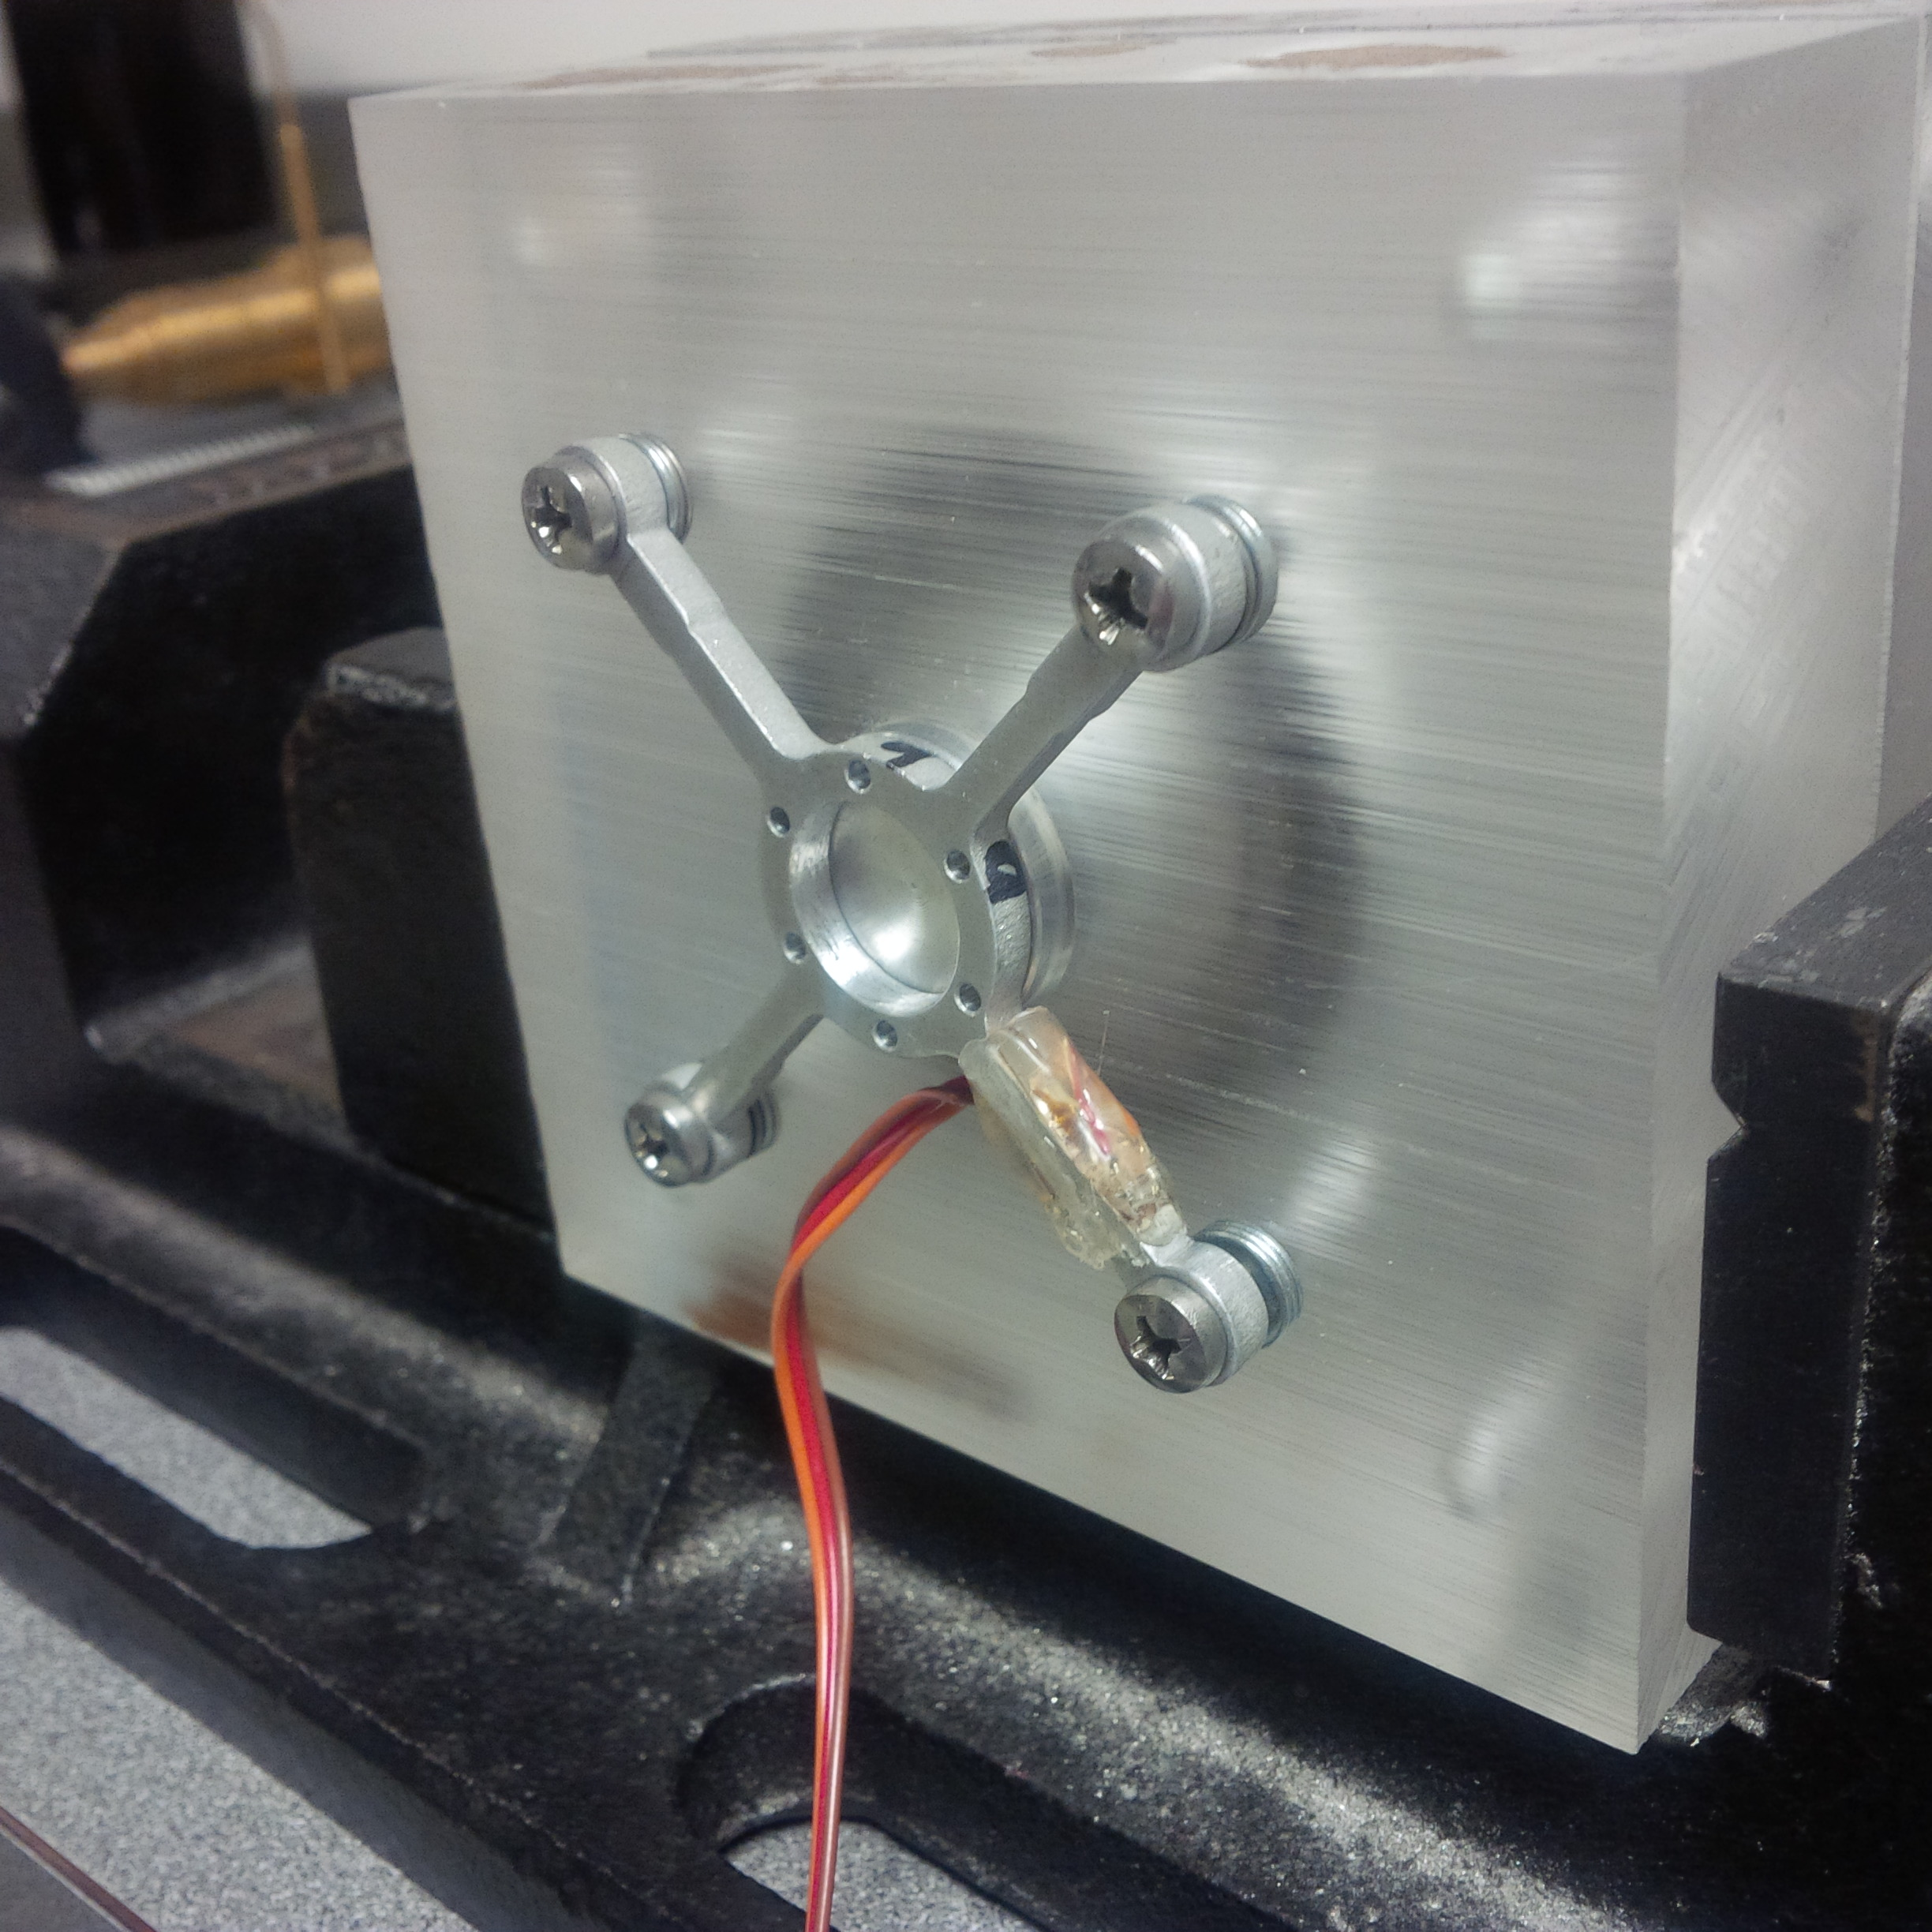
\includegraphics[width=1\textwidth]{./img/test_setup_exposed.jpg}
      \caption{Test setup for the torsional sensor, partially assembled. The four bolts are tightened down, but the center piece rests against a large bearing inside the assembly, to restrict out-of-plane bending.}
      \label{fig:sensor_test_setup_exposed}
    \end{subfigure}
    \begin{subfigure}[b]{0.45\textwidth}
      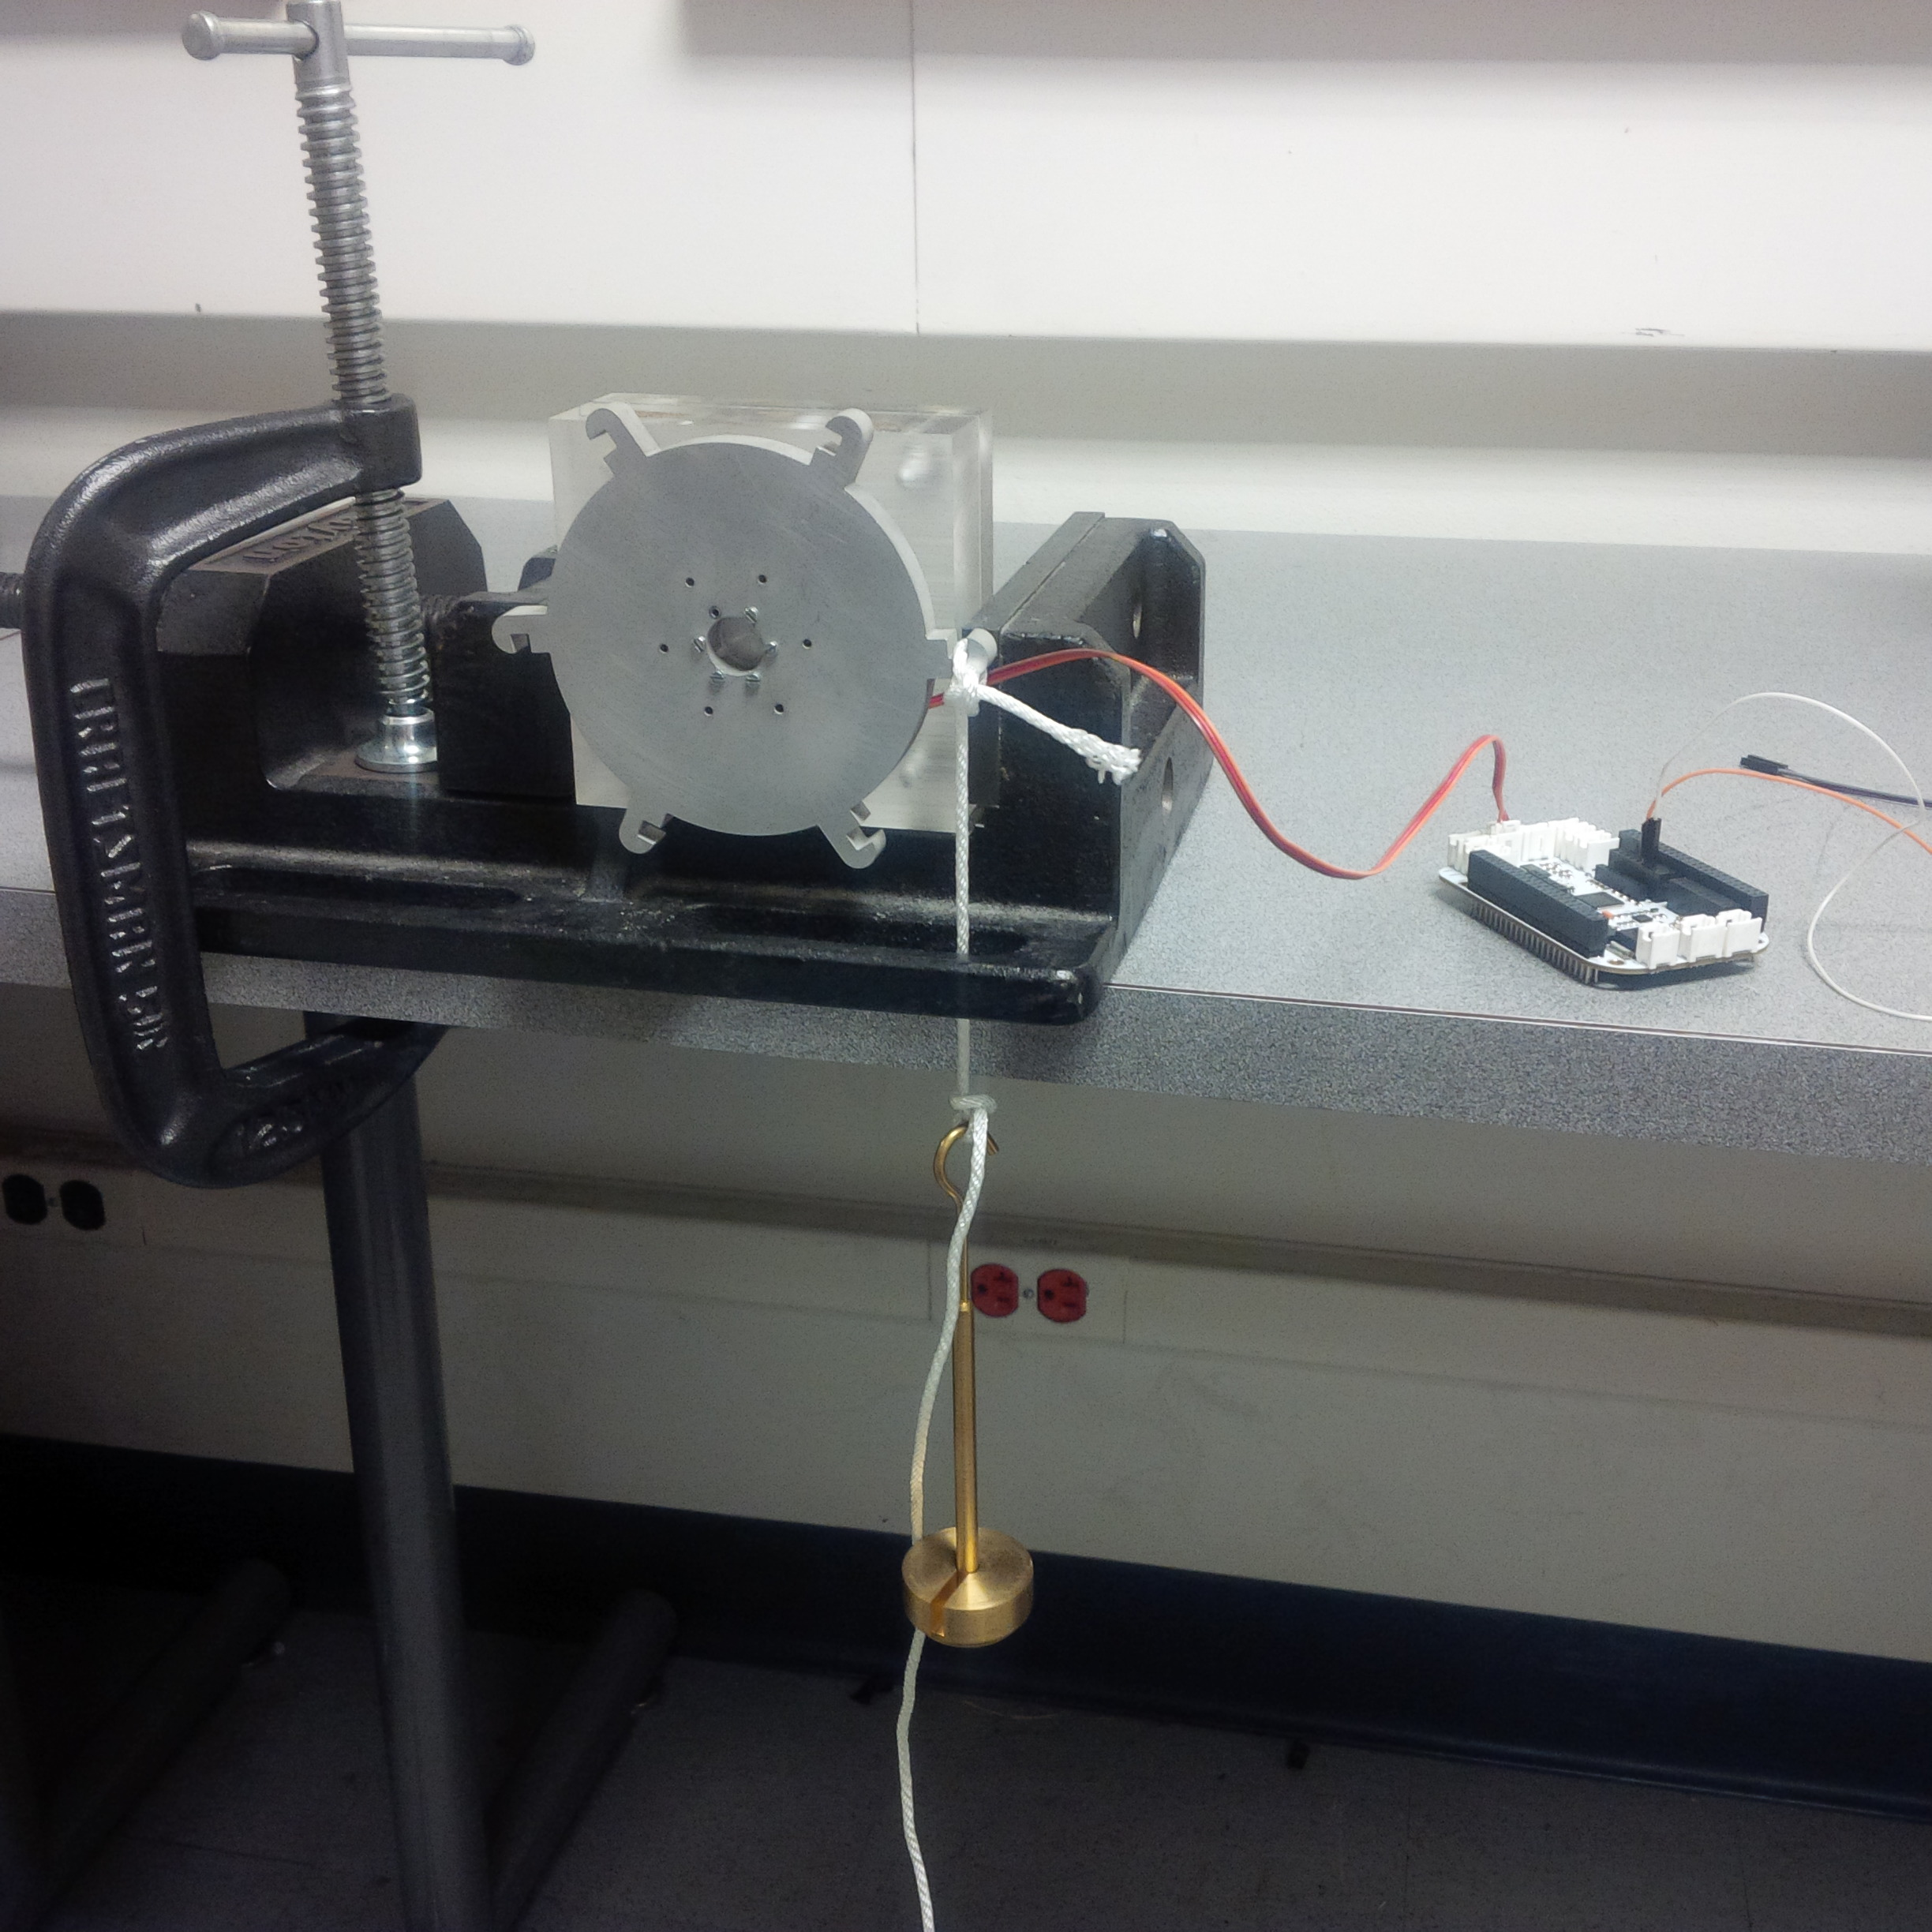
\includegraphics[width=1\textwidth]{./img/test_setup_complete.jpg}
      \caption{Test setup for the torsional sensor, fully assembled, and connected to the data collection PCB. The front piece with hooks for the cord is held onto the torsional sensor by the bolts in the pattern of the motor, and screw into threaded holes in the inner bearing piece.}
      \label{fig:sensor_test_setup_complete}
    \end{subfigure}
  \end{center}
%  \vspace{-0.5cm}
\end{figure}

\subsection{Torsional Sensor Testing In-Situ}

After calibrating each of the 12 torsional motor mount sensors, SUPERball was fully assembled, and one of these sensors was tested to confirm that appropriate readings were being returned.
Figure \ref{fig:sensor1data} shows estimated force (from a 2nd-order curve fit for the know sensor calibration) of a cable when commanded in a square-wave pattern, taken from torsional sensor 1 and transmitted wirelessly from a BeagleBone Black on the robot to a local computer.
This graph matches the actuated square wave reasonably well, although noise and hysteresis are evident without filtering and without implementing a state observer.

\begin{wrapfigure}{R}{0.40\columnwidth}
      \centering
      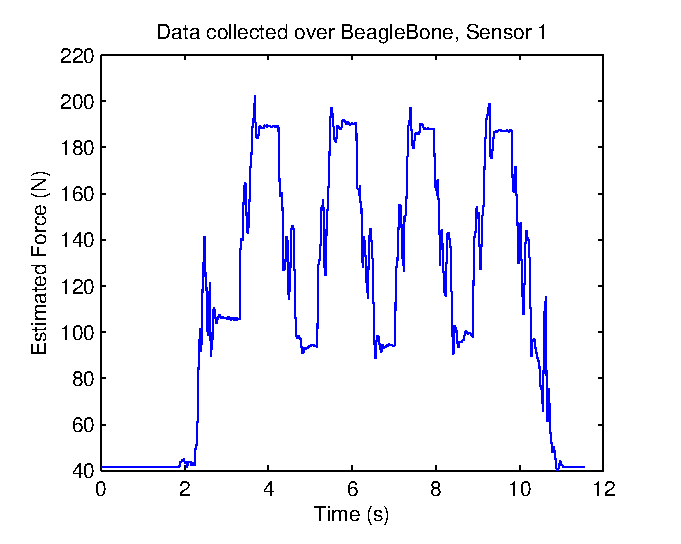
\includegraphics[width=0.6\columnwidth]{img/Force_Time_Graph_adjusted.eps}
      \caption{Motor mount torque sensor data recorded during a square wave input position trajectory for a motor. A square wave of tension is sensed, detecting the commanded position trajectory up to a calibration constant, showing the validity of SUPERball's torque sensors.}
      \label{fig:sensor1data}
      \vspace{-0.4cm}
\end{wrapfigure}

%\section{Qualitative Testing of Fully-Assembled Mechanisms}

%Show images of SUPERball actuating the sinusoid, as an example of the mechanism working.
%Success!

%Discuss external cable bending and hysteresis.

\chapter{Preliminary Locomotion Results}

\begin{figure}[thbp]
    \centering
    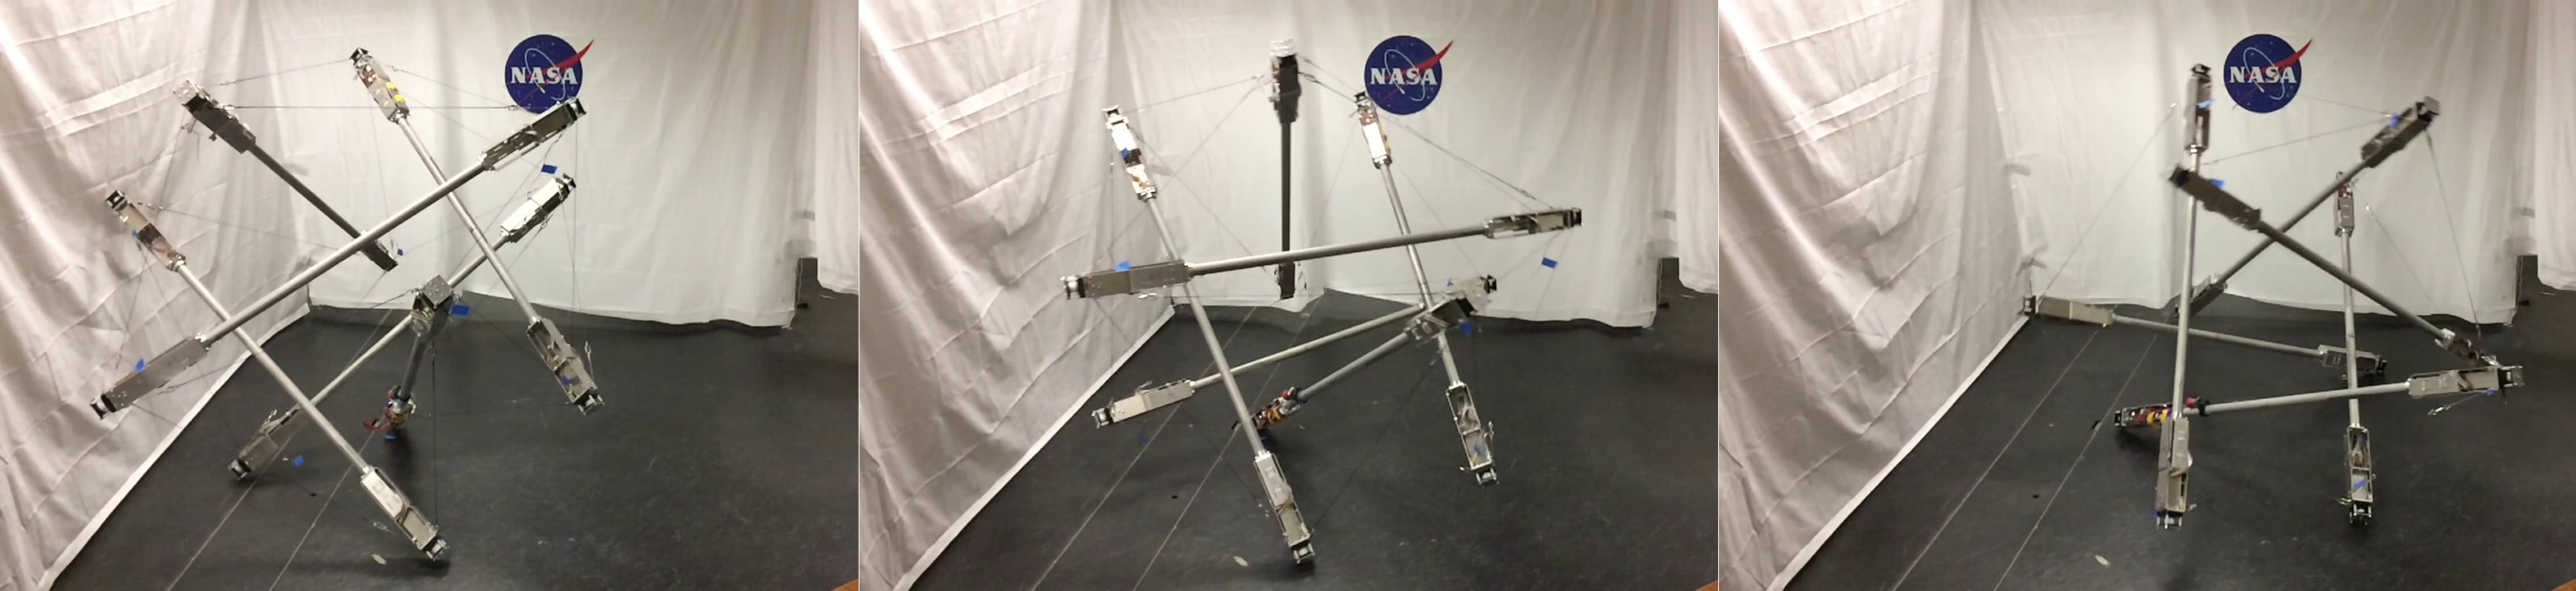
\includegraphics[width=1\linewidth]{img/superball_flop_combined.jpg}
    \caption{SUPERball performing a single \emph{punctuated roll} or face-change movement. The robot starts on one triangular face, and after locomoting forward, stands on a different triangular face.}
    \label{fig:superball_flop_flat}
\end{figure}

Figure~\ref{fig:superball_flop_flat} shows still frames from an experiment where the motor position controller retracts a cable.
The retraction distance required for movement was hand tuned, and will be validated against simulations in future work.
In practice, one single face-change movement required retraction of roughly half of the starting length of one of SUPERball's cables.

In this case, the active cable being controlled is on the bottom triangle, and punctuated rolling is induced when the center-of-mass of the robot moves outside the shrinking triangle base.
Similar to the Berkeley Rapid Prototyping tensegrity kit~\cite{kim2014rapid}, this method represents one motion primitive for spherical tensegrity systems.
Future work will include locomotion in which the dynamics and inertia of rods are used to propel the robot forward, as in~\cite{Iscen2013,Iscen2013b}.

\chapter{Future Research}

Though the mechanisms and sensors in this report allowed for basic single-step locomotion, improvements may be needed before fully dynamic rolling locomotion is possible. 
The following areas are targets of future research.

First, the compressive force sensing system will likely need to be redesigned to avoid the spring buckling sensor noise issue.
This will likely involve either a change in the spring holder tube, or a change in the spring itself.
One possibility for a spring change is to move to an extension spring, since those do not buckle (no compression), but which would involve designing a stopper piece so the spring does not plastically deform past its limit.
And, as mentioned in the sensor testing section for the compression sensor, more designs of the physical sensor itself would be desired such that it does not accidentally deform and lose calibration.

Although the cable exit points from the rod-end were heavily designed to avoid friction and bending, the very exit itself does not enforce a gentle enough bending radius for the cables when they are outside the endcap.
Figure \ref{fig:final_endcap_reverse} shows the exit point of one of these cables.
Note how even though a teflon tube covers the cable exit, both the tube and cable are still bent at an extreme angle.
It may be the case that this unmodelled friction and deformation may prevent accurate state estimation, in which case a redesign or additional design would be needed to guide the cable out more smoothly once outside the rod end.

As described in the experimental testing section, the bottom spool cap flanges shear off under load.
Before drop testing or serious performance testing, these caps will be redesigned with thicker and stronger flanges, as well as to reduce the stress concentrations at the top of the flanges.

Finally, a protective ``shoe'' or ``foot'' is desired for the outermost part of the endcap.
Original designs had included a circular rubber piece that mounted to the top of the cap, but this was deemed to be too expensive and difficult to manufacture.
Without the protective shoe, the actuator housing and bearings are subjected to higher impulses and more dirt and dust.
A feasible design for a protective shoe is likely required before testing in real environments (such as the NASA Ames Research Center Roverscape.)

However, despite all of these future improvements, I and my collaborators believe that this v1.6 of SUPERball represents a significant step forward in the mechanism and sensor design of cable-driven tensegrity systems, and are excited to continue to work towards fully dynamic rolling locomotion.

%Mechanisms to improve:
%- Springs and buckling
%- External cable bending
%- Bottom Spool Cap Failure
%- Protective Rod Shoe

\appendix
\chapter{Additional Reference Material}


\bibliographystyle{unsrtnat}
\bibliography{MastersReport_apsabelhaus.bib}

\end{document}


%to-do: 
% all citations and references - add them
% citations and references - clean up, make sure they are correctly displayed
% figures: adjust
% all blue-text additions
% review hardware testing section and confirm that it's correct
% ACKNOWLEDGE/CITE other collborators' work in all sections! JB, KC, SD, etc.
% motor selection equations / tensegrity design spreadsheet
% list of figures - remove captions?

